\documentclass[a4paper, 12pt, openany]{book} %chose the paper size and font size. Openany ensures that all all chapters and similar may begin at any page, not only odd pages. For the introductory pages and appendices we want openany, but for chapter pages in the main content we want chapters to begin only on odd pages (right hand side). The book class ensures that the margins are automatically adjusted such that left hand pages are slightly moved to the left and vice versa at the right, which makes the thesis very readable and good looking when printed in bound book format.
\usepackage[utf8]{inputenc} %to manage special characters
\usepackage[T1]{fontenc} %to manage special characters
\usepackage[Bjarne]{fncychap} %fancy chapter style (many more available, like Sonny or Lenny etc.)
\usepackage{fancyhdr} %to customize the headers
\usepackage[lmargin=1.5in, rmargin=1in, tmargin=1in, bmargin=1in]{geometry} %sets the margins for the pages
\setcounter{tocdepth}{2} %table of contents number depth for subsections (2 = x.x.x)
\setcounter{secnumdepth}{4} %numbering depth for headers for subsections in the text(4 = x.x.x.x)
\usepackage{url} %to include urls
\usepackage{listings} %include this if you want to include code in the thesis
\usepackage{amsmath,amssymb} %mathematical package
\usepackage{siunitx} %includes SI-units
\usepackage[bf]{caption} %makes float captions bold
\usepackage{array, booktabs} %to make better tables
\usepackage{amssymb}
\usepackage{algorithm}
\usepackage{algpseudocode}
\usepackage{matlab-prettifier}
\usepackage{hyperref}
\usepackage{graphicx} %to include graphics
\usepackage{float} %to include floats
\usepackage{todonotes}
%\documentclass{article}
\usepackage{graphicx}
\usepackage{tabularx}
\usepackage{subcaption}
\usepackage[export]{adjustbox} %to adjust floats
\usepackage{subfig} %to include subfigures
\usepackage{chngcntr} %will make it possible to change the counter for tables, figures etc. such as below
\counterwithin{figure}{section} %change counter for figures within sections (also possible to choose for each chapter
\counterwithin{table}{section} %change counter for tables within sections
\usepackage{color, xcolor} %edit e.g. text colors
\usepackage{tocloft}
\setlength{\cftfignumwidth}{3.55em}

\usepackage[backend = biber,
            style = numeric,
            date = long,     % Long: 24th Mar. 1997 | Short: 24/03/1997
            sorting = none,
            maxcitenames = 3,   % max names to include before et. al.
            ]{biblatex} %customize the look of your citations and bibliography
\addbibresource{bibliography.bib} %declare the bibliography resource
\usepackage{comment} %to be able to comment out sections in the .tex files
\usepackage{afterpage} %to customize page commands such as below
\newcommand\myemptypage{
    \null
    \thispagestyle{empty}
    \addtocounter{page}{-1}
    \newpage
    } %sets new page command to insert an empty page without adding to the page counter or having a page number




\begin{document}
%%%%%%%%%%%%%%%%%%%%%%%%%%%%%%%%%%%%%%%%%%%%%%%%%%%%%%%%
%\begin{comment}
% The title page:
% For NTNU students this page will be generated automatically when submitting your paper, and should not be included in the final file from Latex. Delete or comment out the title page setup. The final report should then start with the first page being the abstract. I have included a title page here so it is possible to see how it may look like, and for those who does not get an automatically generated title page. Of course you will need to change the names and titles etc. to your case.

%the title page should be an odd page (right hand side)

\begin{titlepage}
\newgeometry{left=1.6in, right=2in}
\vspace*{1.5cm}

\noindent  \textcolor{gray}{\large Martin A Kraft} \\
\vspace{1cm}

\noindent \textbf{\Large Control and analysis of PV-microgrid} \\
\vspace{0.5cm}

\noindent {\large Developing a controller for a PV powered microgrid in rural Africa} \\



\vspace{7cm}
\noindent Master's thesis in Engineering Cybernetics \\
Supervisor: Geir Mathisen \\
Co-supervisor: Espen Øverbye \\
February 2024 \\

\vspace{0.2cm}
\noindent Norwegian University of Science and Technology \\
Faculty of Information Technology and Electrical Engineering \\
Department of Engineering Cybernetics \\

\begin{figure}[h]
    \includegraphics[width=0.28\textwidth]{Figures/ntnu_basic.png}
\end{figure}
\end{titlepage}
\restoregeometry
\myemptypage %empty page such that the abstract starts at the first right hand side after the title page
%\end{comment}
%%%%%%%%%%%%%%%%%%%%%%%%%%%%%%%%%%%%%%%%%%%%%%%%%%%%%%%%

% The pre-chapters

\chapter*{Abstract} %pre-chapters should not be numbered, hence the "*"
\addcontentsline{toc}{chapter}{\protect\numberline{}Abstract} %add the chapter to the table of contents, this is not automatically added when creating unnumbered chapters (*). Add it in a chapter style, and keep all chapters on the same numberline indent regardless of number or not on the chapter
\pagenumbering{roman} %introductory pages should be roman
\setcounter{page}{1}
PV-microgrids are proposed as a solution for communities with good solar conditions, but low access to energy infrastructure. A provider of these, Differ Community Power (DCP), wants to introduce an energy management system to their microgrids to increase the life-time and satisfaction from their systems. This thesis looks at an existing system supporting a medical facility in rural Malawi, analyses its operations and proposes an energy management system. The system is tuned to achieve goals developed in collaboration with DCP and the end-user. These goals include a higher availability of critical loads and better battery health. The proposed solution is compared to the existing system in a simulated environment, showing an increase in critical load reliability of up to 2.86 percentage points and a reduction in time in states damaging for the battery of up to 73\% dependent on the tuning. The proposed control system is also tested against the current control system under decreasing amount of battery capacity installed. By a 53\% reduction of battery capacity, the proposed control has a higher critical load reliability of 7.1 percentage points compared to the current system.
\newline
\newline
\newline
PV drevne mikrogrids er en mulig løsning for elektrifisering av områder med gode solforhold der kobling til annen energi-infrastruktur er kostbart eller krevende. Differ Community Power (DCP) er en utvikler av slike mikrogridanlegg. De ønsker å ta i bruk kontrollsystemer for å bedre tilfredsheten og livstidene til systemene deres. Denne oppgaven ser på et av disse anleggene i rurale Malawi og, etter å ha analysert det, foreslår et nytt kontrollsystem. System er stilt til å tilfredstille kriterier utvilket sammen med DCP og deres brukere. Dette inkluderer mål på sikkerheten til kritisk last og batteri-levetid. Det foreslåtte systemet sammenliknes med det eksiterende systemet i et simulert miljø, der det foreslåtte systemet viser en forbedring på tilfredsstillende av kritisk last på 2.86 prosentpoeng og en reduksjon i tiden batteriet er i skadelige tilstander på 73\% avhengig av parametersettingen til systemet. Det foreslåtte kontrollsystemet er også testet mot det eksisterende kontrollsystemet i simulering der installert batterikapasitet er redusert. Med en 53\% reduksjon i batterikapasitet, så viser det foreslåtte kontrollsystemet en forbedring i tilfredstillese av kritisk last på 7.1 prosentpoeng sammanliknet med eksisterende kontrollsystem. 




 %insert the chapter text from the files

\chapter*{Preface}
\addcontentsline{toc}{chapter}{\protect\numberline{}Preface} 
When I enrolled into a 5 year master degree in Engineering Cybernetics at NTNU in the Fall of 2018 I came with a strong interest in robotics and industrial automation. I even choose my specialization within Robot Systems. So why is that I, 5 years later write my thesis on Control of Energy Systems? I attribute this to two key events, the first of which being the Russian Invasion of Ukraine in February 2021 and the resulting shock to our Energy Systems. This event highlighted to me how energy is not to be taken for granted. It made me aware of another consideration to the Energy Transition: Energy Security. Energy Security means the ability to access energy and the reliability and robustness of these sources. The matter of Energy Security differs a lot between regions of the world.  Which brings me to my the second event that steered my academic trajectory into writing this thesis.\\

In waiting to go on an exchange, I was fortunate to be employed at DCP. This employment became prolonged, due to the COVID19-restrictions of my about-to-be host country. The silver lining, I got to travel to Malawi and see the impact of DCPs work. In rural Malawi, energy security and access to energy is no theoretical concern. It is a deep and enduring problem felt every day. When energy is delivered to communities which previously have not had access, the appreciation is deep and profound. 
At the health facilities, nurses told about how in the past cesarean sections at night had to be done with a cell phone light or candlestick in hand. The impact energy can have is literally a matter of life and death.\\

With these experiences in hand, I am very grateful to DCP for allowing me to write my master degree on a topic close to my heart, and that can have real world impact on underserved communities. I want to thank all DCP employees that have through discussions and feedback helped me shape and express my ideas. 

Last,but not least, I want to express my gratitude to my thesis advisor, Geir Mathisen for diligently guiding me throughout the process. 


\tableofcontents
\addcontentsline{toc}{chapter}{\protect\numberline{}Contents}

%add to table of contents list of figures and tables, and insert list of figures and tables
\addcontentsline{toc}{chapter}{\protect\numberline{}\listfigurename}
\listoffigures
\addcontentsline{toc}{chapter}{\protect\numberline{}\listtablename}
\listoftables


\chapter*{Abbreviations}
\addcontentsline{toc}{chapter}{\protect\numberline{}Abbreviations}
% Put in your abbreviations here

List of all abbreviations in alphabetic order:

\begin{itemize}
    \item \textbf{AC} Alternating Current
    \item \textbf{ACF} Auto-Correlative Function
    \item \textbf{ADF} Augmented Dicker-Fuller
    \item \textbf{ANN} Artificial Neural Network
    \item \textbf{ARIMA} Auto Regressive
    \item \textbf{ARIMA} Auto Regressive Integrated Moving Average
    \item \textbf{ASAI} Average Service Availability Index 
    \item \textbf{CC} Charge Controller
    \item \textbf{DCP} Direct Current
    \item \textbf{DCP} Differ Community Power
    \item \textbf{DHI} Direct Horizontal Irradiance
    \item \textbf{DNI} Direct Normal Irradiance
    \item \textbf{DOD} Depth of Discharge
    \item \textbf{DSM} Demand Side Management
    \item \textbf{EMS} Energy Management System
    \item \textbf{EPC} Engineering Procurement Construction
    \item \textbf{FSM} Finite State Machine
    \item \textbf{GIS} Geographic Information System
    \item \textbf{GTI} Global Tilted Irradiance
    \item \textbf{Inv} Inverter
    \item \textbf{KPI} Key Performance Indicator
    \item \textbf{LCOE} Levelized Cost of Energy
    \item \textbf{MA} Moving Average
    \item \textbf{MAE} Mean Average Error
    \item \textbf{MAPE} Mean Average Percentage Error
    \item \textbf{MPPT} Maximum Power Point Tracking
    \item \textbf{NCA} Norwegian Church Aid
    \item \textbf{NTNU} Norwegian University of Science and Technology
    \item \textbf{O\&M} Operation and Monitoring
    \item \textbf{PACF} Partial Auto-Correlative Function
    \item \textbf{PAR} Peak-to-Average Ratio
    \item \textbf{PV} Photovoltaic 
    \item \textbf{PVGIS} Photovoltaic Geographic Information System
    \item \textbf{RMSE} Root Mean Square Error
    \item \textbf{RTH} Receding Time Horizon
    \item \textbf{SAIFI} System Average Interruption Duration Index
    \item \textbf{SAIFI} System Average Interruption Frequency Index
    \item \textbf{SARIMA} Seasonal Auto-Regressive Integrated Moving Average
    \item \textbf{SDG} Sustainable Development Goals
    \item \textbf{SOC} State of Charge
    \item \textbf{STC} Standard Testing Condition
    \item \textbf{UN} United Nations
    \item \textbf{UNICEF} United Nations International Children's Emergency Fund
    \item \textbf{USAID} United States Agency for International Development
    \item \textbf{WFP} World Food Program
\end{itemize}
\newpage
\myemptypage
%add an empty non-counted page by the command below in order to get the first chapter on the left hand side, if needed (check your page number so that the first chapter is on an odd page)


%%%%%%%%%%%%%%%%%%%%%%%%%%%%%%%%%%%%%%%%%%%%%%%%%%%%%%%%
%Customize the layout of the main content of your thesis

\pagestyle{fancy} %set customized page style for header
\fancyhf{} %clear header and footer fields
\renewcommand{\headrulewidth}{0pt} %set to no rule
\fancyhead[LE, RO]{\thepage} %set the page number at left for even, right for odd pages
\fancyhead[RE, LO]{\leftmark} %set the chapter name at right for even, left for odd pages
%is is possible to design the header with the chapter as you wish, e.q. only the chapter or only the name, all lowercase instead etc.
%you could also design the footer if you wish, for example:
%\fancyfoot[LE, RO]{\thepage}
\setlength{\headheight}{14.49998pt} %set the header height


%%%%%%%%%%%%%%%%%%%%%%%%%%%%%%%%%%%%%%%%%%%%%%%%%%%%%%%%
%main content 

\pagenumbering{arabic}
\chapter{Introduction}
\section{Background}

In 2015, the \textit{United Nations} (UN) proposed and adopted the 17 \textit{Sustainable Development Goals} (SDG) in the 2030 Agenda for Sustainable Development\cite{2030agenda} as a succession to the former Millennium Development Goals. Of these, SDG number 7 is about the \textit{availability of affordable and clean energy for all}\cite{un_sdg_7}. While the developed world is looking to replace its current energy supply with cleaner sources, energy, much less clean energy, remains unavailable for large parts of the developing world. This problem is especially acute in Africa. According to the UN report on the SDGs from 2023, 675 million people live without access to electricity, most of which in located in Sub-Saharan Africa.\cite{Desa2023-mr} Many of these live  in rural communities where the regional electricity grid is either unreliable or unreachable. The problem of electrifying these communities, powering and extending the reach of vital services in both health and education, is known as \textit{last-mile-electrification}.\\

Localised, small-scale grid networks using renewable resources have been proposed and developed in several locations where a grid connection is techno-economically infeasible. This is especially relevant in Africa with its abundant solar resources, but lack of infrastructure.\cite{Wang2021-kb} These networks may range from the larger microgrids to the smaller nanogrids depending on the size of the service it is providing. Common for all the solutions is that they provide a self-sustaining system, meaning it can operate without being connected to the larger grid.\\

The company \textit{Differ Community Power} (DCP) is a Norwegian private company looking to develop the technologies and business models to deploy microgrids across rural communities mostly located in rural Sub-Saharan Africa. The company already have more than 100 installations in operation across 8 different countries. The installations are often mounted to support some social infrastructure like health stations, vaccine dispensaries or schools with electricity. The installations are largely funded by multilateral or bilateral organisations and foundations such as UN, WFP, USAID etc. with the recipient government paying a smaller part.\\

In charity and development, it is generally known that it is easier to receive grants to install systems than to operate systems. This is because operation requires larger overhead spending, something organisations and donors loathe. After all, low overhead spending has been perceived as a key indicator of an organisation's effectiveness.\cite{Berrett2020-wi} This is unfortunate for several reasons. First, the competence the company could gain from assessing and evaluating over a longer period is lost. This competence could be used to better operations to offer better products for both the end-user and the customer. Secondly, a longer contract offers the end-user reliability and consistency over a longer period. Lastly, longer contracts create a sense of ownership and facilitate mutual information sharing between user and supplier. This incentivizes the training of the end-user to be able to perform maintenance and repair of the installations. The downsides of the neglect of operations and training have been clear to DCP when installing new systems. Frequently they have arrived at sites with systems already installed, but these are either broken or incomplete.

DCP offers a different approach with a complete package that includes both the \textit{Engineering, Procurement and Construction} (EPC) of the system and a long-term \textit{Operation and Monitoring} (O\&M). Already in place at their sites are systems to monitor the installations. What is lacking, and is of keen interest for DCP to develop, is a framework to analyse and act on, i.e. control, the systems to achieve improved operation on key indicators. This thesis delves into all these points: the analytics of the systems, how they can be controlled for better operation, and what those key indicators should be. 

\section{Motivation}

There are several stake-holders connected to a site, such as end-users, customers and the company DCP itself. Each of these are concerned with different parts of the operation. In this thesis, a series of \textit{Key Performance Indicators} (KPIs) are developed to capture the different interests of the stakeholders. The motivation behind the control system is then to improve the operation with regard to the KPIs. This translates into higher system reliability, availability and lifetime. Something that is of keen interest to all stakeholders.\\

DCP wants to increase the amount of installations in its portfolio. The cost and time required to perform O\&M on the installations increase with the amount of sites. Hence it becomes important to automatize as much as possible. An automated control system aims to fulfil 4 main motivations.\\

\begin{enumerate}
    \item \textbf{Load prioritization}  -    Some loads are critical to fulfilling the purpose of the facility. For instance, medical equipment is critical to fulfil the purpose of a health facility. These are generally deemed as more important by all stakeholders. Currently, these loads are not prioritized, neither in their immediate nor future demand. This means that nothing is stopping less important load from occupying all inverter capacity, or draining the battery so that a critical load cannot run. This is damaging for the end-users because vital services can be unavailable and unreliable. It is damaging for the company because it cannot guarantee to deliver reliable operation of critical load. And it is damaging for the customer because they are not getting the value in terms of human development for their investment.
    \item \textbf{Extend lifetime}  -   As the current control system is not controlling the operation effectively, the electrical system is running in a way which produces unnecessary degradation to various components. Certain components, like batteries, are expensive and prone to damage by unhealthy usage. If one could extend the lifetime of the battery, by improving the operation with regard to its health, it could mean a cost reduction for the long-term O\&M-contract.
    \item \textbf{Enabling additional loads}    -   Because O\&M is costly, DCP is exploring the possibility of offsetting some of that cost by installing additional revenue-generating loads. Examples of these can be rental portable batteries, a solar maize mill or refrigerated storage. The goal of these loads is to provide more streams of income for DCP so that the price of O\&M can be lowered. A control system is identified as a key enabler of such loads because the loads cannot run at the cost of the loads supporting the primary purpose of the installation. A control system could in theory decide to run loads only when surplus power is available.
    \item \textbf{System sizing}    -    Be gaining more insight and the ability to influence system operation, the hope is that this could translate into a more tailored installation size. \textit{(Mehra, V. et al., 2018)} provides a function relating the cost of system unavailability to the cost of various energy sources.\cite{Mehra2018-xs} They find that a control system that can reduce the unavailability of critical loads can justify a lower installed battery and \textit{photovoltaic}(PV)-capacity, reducing the \textit{levelized cost of energy} (LCOE). Most sites are today oversized with regards to production, meaning they most days consume far less energy than the systems could theoretically produce. If one could reduce the system size while keeping reliability and availability above an acceptable level, the cost of the installation could be reduced for the customer. Alternatively, one could provide more services for the end-users, enhancing the value provided by the site.
\end{enumerate}

The process of increasing the amount of loads is already happening, both from the top-down, with the customer donating equipment to support the facility's purpose, or from bottom-up, by end-users such as staff buying electronic devices for their daily life. \textit{Increased access to energy creates a bigger energy demand}. The challenges listed above of system sizing, prioritization and lifetime are only going to become more and more pressing. This thesis arrives at an opportune moment.\\


Provided here is an attempt to design a solution satisfying the issues outlined in the motivation. Specifically this thesis will consider the site of Chiwoza, a small rural health facility located outside the Malawian capital of Lilongwe. The electrical system supporting the operation at the site is studied an analysed. The electrical consumption is analysed through a statistical study and by performing a user survey. The production is studied through a physical model of its sole energy source, a PV-module. The physical model relates the PV-module production with the solar irradiance expected at the site. Based on the analysis a statistical forecasting method is designed to forecast the consumption, while a physical model is developed to forecast production. These are combined with a non-linear optimizer to control the consumption and battery charging. The system is designed using a set of historical data, and then tested by simulation using another, disjoint set of historical data. The results from this simulation show a reduction in unavailability for the critical load, together with better operation for battery health. This although comes with the cost of a higher general unavailability and lower system utilization compared to the current control system. 

\section{Thesis structure}
 In the endeavour of creating a new control system, first, a survey of existing research relevant to the problem is conducted. The literature survey includes related works within \textit{Load analysis, Load Forecasting, Production Analysis, Production forecasting and Energy Management Systems}. The survey is found in \autoref{chap:related_works}. Some deductions and results are included in the proceeding \autoref{chap:theory} to not congest the following chapters. The chapter contains theoretical results on photovoltaic cells, forecasting and battery health used in the rest of the thesis. The subsequent chapters concern the case at hand specifically. In \autoref{chap:system_overview} the current system is outlined. The following \autoref{chap:design} proposes a solution design, with the first part giving the specifications for which the design is to be evaluated. This chapter also includes the necessary analysis for the synthesis of the solution. In \autoref{chap:implementation} the solution is implemented in a simulation environment, with \autoref{chap:results} showing the results of that simulation. These results, together with the design are then evaluated in \autoref{chap:discussion}. This chapter also contains suggestions for future works related to the subject in this thesis. The final \autoref{chap:conclusion} concludes the work done for this thesis.\\

 The main contributions of this thesis are:
\begin{itemize}
    \item \textbf{Propose a control system} yielding improved operations for identified KPIs, with the possibility to adjust the prioritization of the KPIs. 
    \item \textbf{A method for developing load forecasters} using historic data.
    \item \textbf{A proposed physical model for production forecasting}.
    \item \textbf{A system model and simulation} allowing DCP to predict and evaluate their operation.
\end{itemize}

\cleardoublepage
%the cleardoublepage command ensures that the next text page is on the right-hand side (odd page) and produces a blank page if necessary to achieve that, as all chapters should begin on the right hand side


\chapter{Related Works}
\label{chap:related_works}
The topic of microgrid control encompasses several related fields of research such as energy control systems, load and production forecasting and system sizing. On the specific topic of energy control systems for microgrids, studies vary in methodology, control level and in the systems considered. \textit{(Abhishek A. et al. 2020)} outlines in a review paper how microgrid control is usually separated into a 3-layered functionality-based hierarchy. The two initial levels, primary and secondary, work within the microgrid itself to maintain voltage and power balances. The highest level, tertiary, is used to optimize the operation of the grid based on cost, utilization, prioritization etc. The term \textit{Energy Management System} (EMS) is often used interchangeably for the tertiary level. The implementation of the hierarchical control into hardware can be both centralised and decentralised. This thesis will consider tertiary control without concern for hardware implementation.\cite{Abhishek2020-ox}\\

The 2023 review paper by \textit{(Allwyn R.G. et al. 2023)} explores different approaches to tertiary control based on the availability of grid connection and the number of different energy sources connected. If multiple energy sources are connected, such as a system consisting of both solar, wind, battery and grid connection, the operation cost and characteristics of each source are important to consider to achieve optimal operation. Although the site considered in this thesis is only PV-powered, an optimal operation of several energy sources is still relevant for the system considered in this thesis due to the operating cost of the battery. The paper also explores the control from the demand side, known as \textit{demand side management} (DSM).\cite{Allwyn2023-pd}\\

DSM is often performed by implementing price mechanisms to incentivize consumers to shift their consumption to periods more suitable for the microgrid operation\cite{Kanakadhurga2022-op} or by introducing more energy efficient loads\cite{Gilda2018-nh}. \textit{(Wang et al., 2021)} however, argues against the use of price control for DSM in impoverished communities because of the lack of economic flexibility of the consumers. They propose however a classification algorithm to classify consumption based on severity and use targeted approaches to guide consumers into more desirable behaviour. They do not, however, consider an automation of this guidance into a control system that could adjust load depending on the system conditions.\cite{Wang2021-kb}\\

Of the DSM-methods found in the literature survey, most use  a price mechanism to influence behaviour, or the replacement of current loads with more energy-efficient ones. Neither of these are relevant to this thesis which seeks to perform active demand side management by controlling existing loads. The papers by \textit{(Rajbhandari et al., 2022)} and \textit{(Philipo et al., 2022)} however, have a similar case as in this thesis. \textit{(Rajbhandari et al., 2022)} considers a rural microgrid in Nepal and conducts a user survey to classify loads into three levels of priority for the user. A function for user satisfaction based upon load allocation is then used both for allocating energy the day ahead and in real-time. Their control system uses an exhaustive search method to scan through all possible combinations of load and the resulting value of the user satisfaction function. A rules-based method is used to shed low-priority loads if their demand conflicts with the ability to provide for higher-priority loads later and hence decrease user satisfaction. In their experience, the total energy served is reduced, although the system can serve more high-priority loads, leading to a higher user satisfaction score on their user satisfaction function.  The proposed control system solution illustrates an effective and intuitive method to both  control and analyse a system from the demand side. However, there are issues with their design. An extensive search method across all load combinations across the whole time-span will have a large and rapidly increasing complexity. Furthermore, while their solution classifies loads based on priority, other attributes, such as the ability to shift demand are not considered. Loads, where the demand is flexible offer more control options. Neglecting this, as done in the solution, might provide a sub-optimal solution.\cite{Rajbhandari2022-oo}\\

On the other hand, \textit{(Philipo et al., 2022)}  does include both the priority and other key control characteristics in their load analysis of microgrids in East Africa. The two key characteristics were defined to be the ability to shift demand in time and interrupt a load after starting it. Their goal was to perform load shifting and peak clipping to have the load curve fit better the PV-production curve. This they achieved through an artificial neural network algorithm that used the irradiance and expected demand curves as input and produced a real-time updated scheduling of loads. The result was a decrease in peak-demand and peak-to-average ratio (PAR) of 31.2\% and 7.5\% respectively. The paper highlights the possible gains by classifying and controlling loads based on more characteristics than their priority. However, the solution does not attempt to forecast consumption and production, or deal with a larger set of control objectives such as battery lifetime.\cite{Philipo2022-rx}\\

When several energy sources are present, the problem of controlling these is known in the literature as energy management. Common for microgrids, an EMS is tasked with optimally combining a renewable and intermittent energy resource, such as wind or solar, with a dispatchable resource such as a diesel generator or grid. Both \textit{(Sadek SM. et al., 2020)} and \textit{(Salazar A. et al., 2020)} consider a microgrid system of this type in their papers, and aim to construct an EMS minimizing fuel cost. In \textit{(Sadek SM. et al., 2020)} a microgrid system consisting of both a wind and PV-module together with a diesel generator is modelled based on both their active and reactive power. A non-linear optimization problem is constructed aiming to minimize fuel cost, the cost of shedding loads and the cost of curtailing renewable resources. They find an improvement in results when considering reactive power as opposed to when not. While the non-linear optimisation problem set-up is relevant, the scale and inclusion of reactive power is out of the scope of this thesis.\cite{Sadek2020-wl}
The paper by \textit{(Salazar A. et al., 2020)} have a smaller system and range of objectives, they have also included a methodology for production forecasting. In their study, they developed and compared the performance of a rules-based control method with a non-linear optimization approach on a system with photovoltaic power, batteries and a fuel-based generator to support a residential load. The control system combines an optimal energy management problem with a stochastic formulation of the PV-production. The optimal energy problem is formulated as a \textit{receding time horizon} (RTH) non-linear optimization problem where the power to and from the battery is the selection variable and fuel-based power generation is minimized. The dynamic nature of PV-production is captured by a Markov model. The optimization problem is solved by dynamic programming. Compared to the rules-based control, the stochastic optimal energy management system managed to decrease both generator usage and increase battery power availability.\cite{Salazar2020-al}
Both of these studies provide a relevant control method with their use of non-linear optimization. The cases differ though from the one in this thesis, as both papers include several sources of production.\\  

Quite a few studies have looked at various methods for load forecasting in microgrids. \textit{(Dutta et al., 2017)} Used a simple persistence technique to forecast both load and production in a microgrid. Their forecasts used the average of several days prior as look-back time. In their experiment, they vary both the look-back time and the forecast horizon. Their results showed a Mean Absolute Percentage Error of $2.42\%$ for the load forecasting with a look-back time of one time-step. Their method was poor in responding to changing conditions, especially for weather-dependent power prediction.\cite{Dutta2017-oi}\\

In a more complicated approach, \textit{(Zuleta-Elles et al, 2021)} used and compared a \textit{Auto Regressive Integrated Moving Average} (ARIMA) model and a \textit{Artificial Neural Network} (ANN) model to forecasting consumption in a microgrid. They developed different ARIMA models for the various forecasting horizons, some also with a seasonal component, turning it into a seasonal ARIMA (SARIMA) model. The ANN model developed was a 3-layer model with 96 regressors, each representing the load consumption within the past 24 hours, meaning 96 blocks of 15 minutes. Over various forecast horizons, they compared the best ARIMA model to the ANN model in terms of RMSE and MAE. Their results showed that the ANN model outperformed the ARIMA on all prediction horizons except 12 hours ahead. \cite{Zuleta-Elles2021-qh}\\

There are several approaches to PV-production forecasting, including statistical, physical and machine learning. \textit{(Huang et al., 2021)} did a comparative study between a physical model and a neural net model that they developed. The physical consisted of an irradiance model based on the position of the sun, and the solar panels modelled as a diode. They tested their model under both numerical weather predictions and with measured irradiance and temperature. When comparing the physical model to the neural net model, the physical model performed worse when receiving just numerical weather predictions, but better when receiving irradiance- and temperature measurements.\cite{Huang2010-lv} Their method did however not consider system losses, meaning energy lost within the system, which is a key factor in reducing available production for PV-microgrids. 
In the review paper from \textit{(Maghami et al., 2016)} the authors identify several loss factors including losses from shading, wiring and soiling. Of these, the authors find that shading has the potential for the largest losses, ranging between 10-70\% in some studies. The problem of soiling is found to be dependent on the region, where some regions, including sub-Saharan Africa, experience a high degree of soiling due to high dust intensity. The effect of soiling on the production depends on the angle and thickness of the dust layer, ranging from 1-26\%.\cite{Maghami2016-pq} In the 2011 paper by \textit{(Chimtavee A. and Ketjoy, N, 2012)} the authors perform a case study on a PV-microgrid system in Thailand. Over a year, they measured the irradiance and the power consumed by the PV-system. Their results showed an average loss of $26.27\%$ comparing the expected power given measured irradiance to the actual power consumed.\cite{Chimtavee2012-gg}\\ 



From the literature study, the necessity of classifying loads both into their importance and control characteristics, as done in \textit{(Philipo et al., 2022)}\cite{Philipo2022-rx}, is considered valuable input for the control system designed in this thesis. Similarly, it builds upon the usage of a SARIMA-model as in \textit{(Zuleta-Elles et al, 2021)}\cite{Zuleta-Elles2021-qh} for load classification and the physical forecasting described by \textit{(Huang et al., 2021)}\cite{Huang2010-lv}. The physical model is modified based on the loss findings by \textit{(Chimtavee A. and Ketjoy, N, 2012)}\cite{Chimtavee2012-gg}. The receding time horizon optimization from \textit{(Salazar A. et al., 2020)}\cite{Salazar2020-al} is taken as inspiration for the optimizer in this thesis, although the  control objectives and options in their case differ from those in this thesis.\\

The literature survey yielded no study on PV-microgrids without generators or grid connection which combines load shaping and prioritization and battery charge management. This thesis builds upon insight into load and production analysis and forecasting, and energy management systems, and combines this into a, to the best of the author's knowledge, novel application.





\cleardoublepage

\chapter{Theory}
\label{chap:theory}
\section{Photovoltaic cells and Irradiance}\label{seq:pv_and_irradiance}

A photovoltaic (PV) cell is a component generating electricity from light by the photovoltaic effect. A PV-cell, illustrated in figure \ref{fig:pv-effect} consists of two semi-conductors, one with a surplus of electrons, the negative(N)-side, and one with a deficit, the positive (P)-side. Between the two semi-conductors is an electric field. Photons from sunlight energize the atoms on the N-side, freeing up an electron. This electron then travels through the circuit to the P-side, creating an electric current to be utilized by external loads.\\

\begin{figure}
    \centering
    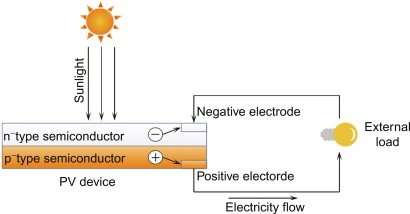
\includegraphics{Figures/06Design/pv_effect.jpg}
    \caption[PV-effect]{Illustration of the PV-effect. Figure from \textit{(Asdrubali, F. et al. 2019)} \cite{Asdrubali2019441}}
    \label{fig:pv-effect}
\end{figure}

The power produced by a PV-cell correlates with the power received from the sunlight.\cite{Frederick1995} The power per area is known as irradiance and is measured in $W/m^2$. There are different types of solar irradiance including
\begin{itemize}
    \item \textit{Global Tilted Irradiance(GTI)}    -   The total irradiance received on a surface with a given azimuth and slope.
    \item \textit{Direct Normal Irradiance(DNI)}    -   The irradiance measured on a surface element perpendicular to the sun's direction. Excludes irradiance scattered by the atmosphere. Dependent on weather and atmospheric conditions such as cloud cover.
    \item \textit{Diffused Horizontal Irradiance(DHI)}  -   The irradiance received on a surface element from light scattered by the atmosphere. Just as DNI, dependent on atmospheric conditions.
\end{itemize}

There are several methods for modelling the total irradiance(G) on a PV-panel given the GTI, DNI, DHI and weather conditions. In the paper \textit{(Frederick, J. E., and H. D. Steele, 1995)} the authors used the simple equation

\begin{equation}
    G = f*G_{DHI} + (1-f)*G_{GTI}
    \label{eq:irradiance}.
\end{equation}

Where $f$ is the cloud cover, $N_{DHI}$ the DHI and $N_{GTI}$ the GTI at the time of measurement. 

\section{Forecasting}
Forecasting is the process of making future predictions based on present or past information. Applied to microgrid control, this often means predicting the value of future demand and production. To be able to make accurate forecasts for these values is of crucial importance to effectively controlling the system. 

There are several different approaches to time-series forecasting. Amongst these are statistical and physical approaches. 

\subsection{Statistical approach}\label{seq:stat_forecasting}

\textit{Statistical forecasting} relies primarily on the historic values of a time-series to predict its future value. They assume an \textit{auto-regressive property}, meaning that a future value can partially be predicted based on past values.\\

A \textit{persistence model} is the most direct implementation of this assumption. It assumes that the current and historical conditions are similar  to some future ones. This is sometimes known as the naive approach and is mathematically expressed in equation \ref{eq:persistence}. The model can be  extended into an \textit{average model} by using the average over the past number of days to estimate the future value, as done in equation \ref{eq:persistence_avg}. For an average model, the key parameter to select is the \textit{look-back period}, meaning the amount of past terms to include in the calculation of the future value. In equation \ref{eq:persistence_avg} this is the \textit{k}-parameter. Additionally, a weighting of the different terms in the average model can be introduced to produce a \textit{weighted persistence model}. This, as shown in \ref{eq:weighted_persistence_avg}, will vary the impact of the different past terms for the final forecast. While allowing more flexibility, this is significantly more difficult to tune, as the weight vector will have equal length to the target vector. It is possible to simplify this by defining the weight as a function.    

\begin{equation}
    \hat{x}_{t+1} = x_{t}
    \label{eq:persistence}
\end{equation}

\begin{equation}
    \hat{x}_{t+1} = \frac{1}{(t-k)}\sum_{i=k}^{t}{x_t}     ,t>k>0
    \label{eq:persistence_avg}
\end{equation}

\begin{equation}
    \hat{x}_{t+1} = \frac{1}{(t-k)}\sum_{i=k}^{t}{w_i x_i}     ,t>k>0
    \label{eq:weighted_persistence_avg}
\end{equation}

An \textit{Auto-Regressive Integrated Moving Average (ARIMA) model} is a more complex statistical model and a commonly used framework for forecasting. It consists of an \textit{Auto-Regressive model} and a \textit{Moving-Average model}, with an integrated term. 

An auto-regressive model predicts the future value of a variable from the historical values of the variable. It is the same as the \textit{weighted persistence model} defined above. It is often denoted as AR(p) where p represents the order of the model i.e. how many past terms are included. Equation \ref{eq:ar_model} expresses this mathematically. 

A moving average model is most useful when a variable oscillates around some average $\mu$. It uses the average and the past deviation from the average to estimate the variable. Similar to an AR-model, a moving average model can have different orders and is denoted as MA(q) with a mathematical expression as seen in \ref{eq:ma_model}.

Lastly, the integrated term of the ARIMA is used if the original time-series expression has non-\textit{stationary} attributes. A stationary time-series has a time-invariant mean and variance. There are different kinds of stationarity, such as \textit{wide-sense stationarity}, which allows for cyclic behaviour within a time-series as long as the series is stationary across the period. Both the AR- and the MA model require a stationary time-series to perform optimally. If the time-series itself is not stationary, meaning that the mean or variance is time-variant, a differentiated time-series with values expressed by equation \ref{eq:differencing} for either a 1. or 2. order difference can be utilised to remove the non-stationary components. The order of the differentiating term can be written as I(d). Together with the AR and MA model, an ARIMA model of order p,d and q can be written as ARIMA(p,d,q).
\begin{equation}
    x_t = \sum_{i=1}^{p}{\phi_i x_{t-i}} + \epsilon_t
    \label{eq:ar_model}
\end{equation}

\begin{equation}
    x_t = \mu + \sum_{i=1}^{q}{\theta_i \epsilon_{t-i}} + \epsilon_t
    \label{eq:ma_model}
\end{equation}

\begin{align}
    x_t' &= x_t - x_{t-1}        (1.order)\notag\\
    x_t^* &= x_t' - x_{t-1}'     (2.order)
    \label{eq:differencing}
\end{align}

An ARIMA can be extended to account for seasonal components of a time-series. Such a model is known as a seasonal ARIMA (\textit{SARIMA}) model. In addition p,d and q coefficients, the SARIMA has the additional P, D, Q and a seasonality constant. Similarly to the coefficients for the regular  ARIMA, these coefficients define how many terms are to be included for the AR, I and MA models respectively, only that they are shifted backwards by the seasonality constant. 

\subsubsection{Model and parameter selection ARIMA}\label{seq:tuning_arima}
There are several methods for choosing the appropriate model and parameters for an ARIMA model, one of the most common is the \textit{Box-Jenkings method}. The Box-Jenkings method is a step-wise algorithm for choosing the best fit ARIMA-model. The first step is model identification and selection. This means finding the correct values for the ARIMA-parameters \textit{p,d,q,P,D,Q and s}. A prerequisite for selecting these parameters is to examine the seasonal and stationary behaviour of the time-series.\\ 

The seasonal behaviour is often known a priori, but if not it can be inferred through an ACF plot by examining the terms within a confidence interval. It is the length of the period over which the pattern repeats itself. In our systems, we know in advance that both demand and production follow a daily cyclic pattern. This yields the seasonal parameter \textit{s}.\\

Both the AR- and MA-model perform sub-optimally if the time-series exhibits strong non-stationary behavior.  If a series is wide-sense stationary, an ARMA model is in theory sufficient for forecasting. Stationarity can be determined from a time-series plot, but there are also tests developed. One of the test for stationarity is the \textit{Augmented Dicker-Fuller}-test (ADF-test).\\ 

The ADF-test test the null hypothesis that the unit root is part of the process' characteristic equation. If the null hypothesis is accepted, it means that the unit root is present, and the process is non-stationary. On the other hand, the null hypothesis might be rejected. The test statistic $\mathbf{DF}$ obtained from the test indicates how strongly the null hypothesis is rejected. If this is more negative than some critical value, it indicates that the process is stationary. The result of this process is the order of differentiating, the \textit{d}-term. A key point regarding differentiating is although it can achieve better stationarity, it may remove some of the information from the time-series.\\

When the stationary and seasonal behaviour of the process is determined, then the order of the AR and MA models can be obtained from the partial auto-correlation function (PACF) and auto-correlation function respectively.\cite{Zuleta-Elles2021-qh}\\

The order of the auto-regressive model can be found in the partial auto-correlation function. The PACF gives the direct correlation between a past term $x_{t-k}$ and the target term $x_t$ removing any indirect effect through intermediate terms $x_{t-1},..., x_{t-k+1}$. The order of the AR model only includes terms with a statistically significant direct effect on the target term. Its connection to the PACF is therefore intuitive as the PACF will only show terms above a confidence interval if they have a statistically significant effect on the target term. Hence its order is equal to the amount of terms of the PACF before the PACF goes outside the confidence interval. This will yield the \textit{p}-term of the ARIMA-model.\\
%\todo{Show plots?}

The order of the moving average model, on the other hand, can be determined from the auto-correlation function. The ACF gives the correlation between a past term $x_{t-k}$ and the target term $x_t$, including both the direct effect and the indirect effect through intermediate terms. The connection between the ACF and the order of the MA-model is less intuitive than that between the PACF and AR-model. The following is an attempt to connect the two based on the method in \cite{Ritvikmath2019-np}:\\

Consider a MA(q) model as described by equation \ref{eq:ma_model}. Expanded, this will look like
\begin{equation}
    MA(q): x_t = \mu + \theta_{t-1} \epsilon_{t-1} + ... + \theta_{t-q} \epsilon_{t-q} + \epsilon_t
    \label{eq:ma_model_expanded}.
\end{equation}

The ACF gives the correlation between the target term and past terms. The correlation between $x_t$ and $x_{t-l}$ can be written as

\begin{equation}
    Corr[x_t,x_{t-k}]   =   \frac{Cov[x_t,x_{t-k}]}{\sigma_{x_t}\sigma_{x_{t-k}}}
    \label{eq:ma_corr}.
\end{equation}

Assuming a non-zero variance, the denominator of \ref{eq:ma_corr} will be some constant. For selecting the order of the MA-model, we are interested in when the ACF is zero. The denominator can therefore be neglected, and we are left with a proportional equation as

\begin{equation}
    Cov[x_t,x_{t-k}]    =   E[x_t x_{t-k}] - E[x_t] E[x_{t-k}]
    \label{eq:ma_cov}.
\end{equation}

The $E[x_t]$-term can be expanded as

\begin{align}
    E[x_t] & = E[\mu + \theta_{t-1} \epsilon_{t-1} + \ldots + \theta_{t-q} \epsilon_{t-q} + \epsilon_t ] \notag \\
           & = E[\mu] + \theta_{t-1} E[\epsilon_{t-1}] + \ldots + \theta_{t-q} E[\epsilon_{t-q}] + E[\epsilon_t]
    \notag \\
           & = \mu + \theta_{t-1} E[\epsilon_{t-1}] + \ldots + \theta_{t-q} E[\epsilon_{t-q}] + E[\epsilon_t].
\end{align}

As the error of a stationary process is assumed to be unbiased, every term involving $E[\epsilon]$ is therefore equal to zero. We are left with

\begin{equation}
    E[x_t] = \mu.
\end{equation}

Equation \ref{eq:ma_cov} can therefor be written as 

\begin{equation}
    Cov[x_t,x_{t-k}]    =   E[x_t x_{t-k}] - \mu^2
    \label{eq:cov_semi}.
\end{equation}

The $E[x_t x_{t-k}]$ is more complicated. Using the definition in \ref{eq:ma_model_expanded}, the product $x_t x_{t-k}$ can be written as 

\begin{align}
    x_t x_{t-k} &= (\mu +\theta_{t-1} x_{t-1} +...+\theta_{t-q}x_{t-q})(\mu +\theta_{t-k} x_{t-k} +...+\theta_{t-k-q}x_{t-k-q})\notag \\
    &= \mu^2 + \mu(\theta_{t-k} x_{t-k} +...+\theta_{t-k-q}x_{t-k-q})\notag\\
    &+\theta_{t-1}x_{t-1}(\mu+\theta_{t-k} x_{t-k} +...+\theta_{t-k-q}x_{t-k-q})+...\notag\\
    &+\theta_{t-q-1}x_{t-q-1}(\mu+\theta_{t-k} x_{t-k} +...+\theta_{t-k-q}x_{t-k-q})
    \label{eq:cov_product}.
\end{align}

The $\mu^2$ from \ref{eq:cov_semi} and \ref{eq:cov_product} will cancel each other out. From equation \ref{eq:cov_product} we are then left with three kinds of terms when inserted into \ref{eq:cov_semi}: Either 
\begin{align}
    I: & \mu \theta_{t-r}E[x_{t-r}], r=1,2...q\notag\\
    II:& \theta_{t-r}\theta_{t-l}E[x_{t-r}x_{t-l}], l\neq r\notag\\
    III:& \theta_{t-r}^2E[x_{t-r}^2].
\end{align}

Because the errors are independent of each other and unbiased, terms $I$ and $II$ are equal to zero. The only terms that will not be equal to zero is the $III$ terms, because that would imply zero variance. These terms will only appear if $x_t$ and $x_{t-k}$ have overlapping terms. Going back to \ref{eq:cov_semi} we have that

\begin{align}
    Cov[x_t,x_{t-k}] \neq 0 \iff t-q\leq t-k \implies k\leq q.
\end{align}

This then means that from the ACF, the only way to get a non-zero value is if the term is less than or equal to the order of the MA-model. Hence the \textit{q} from the MA-model may be determined from the ACF.

The terms for the seasonal component \textit{P,D and Q} can by determined through the same process as for the non-seasonal, but looking at the behaviour one period back. The ACF and PACF will often have a spike at a lag of one period, this may then be included as the order of the seasonal model. If the model is trending between seasons, a seasonal differtiating term of order \textit{D} may be included.


\subsection{Physical approach}\label{seq:physical_forecasting}
\textit{Physical models} on the other hand are built on the physics of the system. The forecast is therefore based on the system dynamics and external input. In this thesis, a physical model is used to predict power production from the solar panels based on solar irradiance. Therefore, an outline of the relationship between solar irradiance and power is included here.\\

Irradiance is measured in power over area $(W/m^2)$. The irradiance cast onto the panels depends on the location, orientation and angle of the panels, in addition to the weather conditions. The amount of the irradiance that is converted to electrical power is dependent on total panel size and efficiency, this is given by \ref{eq:pv_power_simple}. The efficiency $\eta$ is often found during the testing of the panels. It is expressed in \ref{eq:pv_efficency} where $P_{STC}$ and $G_{STC}$ represent the power and irradiance under \textit{standard testing conditions} (STC) respectively. Together, that gives the complete equation for the power given by each panel seen in \ref{eq:pv_power_full}. 

\begin{equation}
    P = \eta A G
    \label{eq:pv_power_simple}
\end{equation}

\begin{equation}
    \eta =  \frac{P_{STC}}{A G_{STC}}
    \label{eq:pv_efficency}
\end{equation}

\begin{equation}
    P = \frac{P_{STC}}{G_{STC}} G
    \label{eq:pv_power_full}
\end{equation}


Specifically for the case considered in this thesis, we want to obtain a predicted time-series of the production for some time into the future. 

\subsection{Error metrics for forecasting}
It is crucial to be able to evaluate a forecast, to assess the suitability of a forecaster. This is in general done by comparing the forecasted time-series $F$ to the actual time-series $A$. The measurement error $\varepsilon_i$ at time-step $i$ is defined in equation \ref{eq:measurement_error}. One could find the error for all measurements and combine them into a vector. This will yield an error vector equal in size to the $A$ and $F$. It is common to reduce the errors for all samples into a single error statistic. The most common of these are \textit{Root Mean Square Error} (RMSE), \textit{Mean Average Error} (MAE) and \textit{Mean Average Percentage Error} (MAPE). The difference between these in their intuition and accuracy requires an informed decision about the choice of error metrics.

\begin{equation}
    \varepsilon_i = A_i - F_i
    \label{eq:measurement_error}
\end{equation}

MAPE, shown in equation \ref{eq:mape}, is perhaps the most intuitive, as the percentage error will follow the scale of the measurements. It has however a few major drawbacks.\cite{MAKRIDAKIS1993527} As discussed in \textit{(Makridakis, S., 1993)}, MAPE is poorly suited to compare different models as it will systematically bias towards forecasts lower than the actual time-series. This is because it punishes over-estimates harsher than under-estimates. Consider a situation with an actual timeseries $A$ and a forecasted series $F$ with $A_1 = 1$, $A_2 = 3$ and $F_1 = F_2 = 2$. The absolute percentage error between $A_1$ and $F_1$ is $\frac{|A_1-F_1|}{A_1}*100\%=100\%$, between $A_2$ and $F_2$ however it is $\frac{|A_2-F_2|}{A_2}*100\%=33.3\%$\cite{kolassa2011}. This shows that the same absolute deviance from the actual time-series receives a higher MAPE if the forecast is above, than if it is below the actual value. There have been efforts to avoid this bias, however then at the loss of the intuitive appeal of the method.\\

Both RMSE and MAE, shown in equation \ref{eq:rmse} and \ref{eq:mae} respectively are better suited because they avoid this bias. These methods are fairly similar to each other, however, the MAE has some advantages making it more appropriate. First of all, it is arguably more intuitive than the RMSE. Secondly, it varies proportionally with the absolute error, while the RMSE does not as it also varies with the root of the number of errors\cite{Willmott2005-go}.

\begin{equation}
    \text{RMSE} = \sqrt{\frac{1}{n} \sum_{i=1}^{n} (\varepsilon_i)^2}
    \label{eq:rmse}
\end{equation}

\begin{equation}
    \text{MAE} = \frac{1}{n} \sum_{i=1}^{n} |\varepsilon_i|
    \label{eq:mae}
\end{equation}

\begin{equation}
    \text{MAPE} = \frac{1}{n} \sum_{i=1}^{n} \left|\frac{\varepsilon_i}{A_i}\right| \times 100
    \label{eq:mape}
\end{equation}




\section{Reliability and System Sizing}\label{sec:reliability}
Reliability describes the ability of a system to function under stated conditions. There are several methods for measuring reliability over some period of time, amongst these are:
\begin{itemize}
    \item \textit{System Average Interruption Frequency Index} (SAIFI)    -   The average number of interruptions that occurred per system.
    \item \textit{System Average Interruption Duration Index} (SAIDI)    -   The length of interruptions per system.
    \item \textit{Average Service Availability Index} (ASAI)    -   The average unavailability of supply from a system, or parts of a system, compared to the total demand. 
\end{itemize}

If the loads are stratified based on priority, the reliability can be subdivided into reliability for types of loads such as critical reliability for critical loads, non-critical reliability for non-critical loads and total reliability for all loads. In microgrid systems, the reliability is dependent on the relationship between energy production, storage and consumption. In \textit{(Mehra, V. et al., 2018)} the reliability of a PV-microgrid system is described by a function of installed PV and Battery capacity visualised as in Figure \ref{fig:mehra_reliability_full} where the function values are found through simulation.\cite{Mehra2018-xs}. 

Such a function allows for a structured approach to system sizing, for instance through optimization. The authors in \textit{(Mehra, V. et al., 2018)} propose an optimization formulation minimizing the installation cost while preserving reliability above a certain threshold. The optimization problem is shown in equation \ref{eq:size_minimization} where $c, c_{k}$ and $c_{l}$ are the total cost, cost of Battery capacity and PV-capacity respectively. $B$ is the battery capacity while $PV$ is the $PV$ is the PV-capacity. The $TR$ represents the total reliability and the $CR$ the critical load reliability, here set to be no less than 90\% and 99\% respectively.\textit{(Mehra, V. et al., 2018, p.81)}\cite{Mehra2018-xs}

\begin{figure}[h]
    \centering
    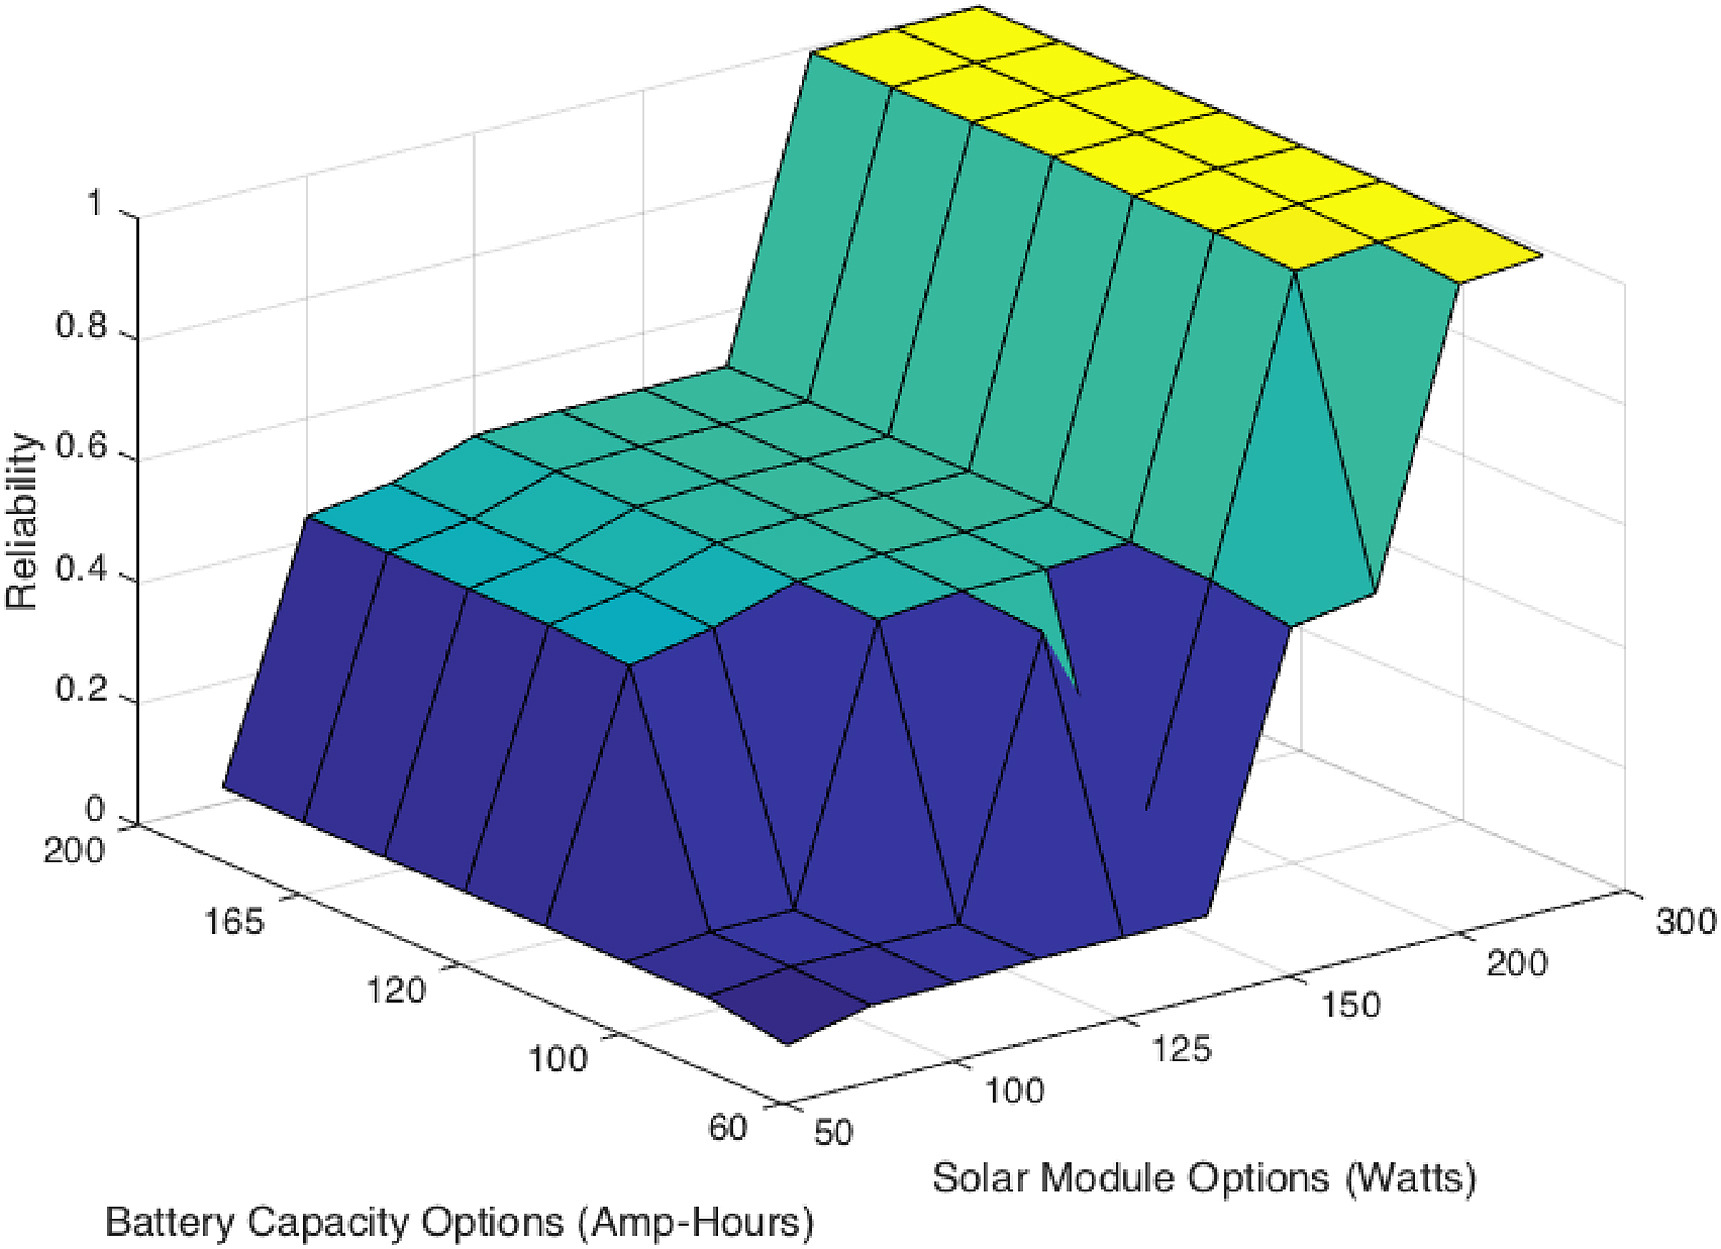
\includegraphics[width=\textwidth]{Figures/05Theory/mehra_reliability_full.jpg}
    \caption[Critical Load Reliability Plot]{Critical load reliability plot from \textit{(Mehra, V. et al., 2018 p.82)}\cite{Mehra2018-xs}. Reliability is expressed here as a function of PV and Battery Capacity, taking values from 0 to 1.}
    \label{fig:mehra_reliability_full}
\end{figure}

\begin{align}
    \min_c\hspace{0.5cm} & c = c_k * B + c_l * PV\notag\\
    \text{s.t.  } & TR \geq 90\%\notag\\
    & CR \geq 99\%
    \label{eq:size_minimization}
\end{align}


\section{Battery Health}\label{seq:battery_health}

Batteries are complex electrochemical components storing energy. The total charge of a battery is described in \ref{eq:battery_lifetime} as how low one can drain the battery, i.e. \textit{Depth of Discharge (DOD)}, multiplied by the number of cycles a battery is expected to last. Batteries are therefore components with a natural lifetime, which will gradually decline with usage. There are however additional effects that may accelerate the deterioration more rapidly than the natural usage. As batteries are amongst the most expensive equipment of a microgrid, it is of great value to control the microgrid in such a way as to not decrease the expected lifetime beyond its natural degradation. \\

\begin{equation}
    E_{tot} = DOD * n_{cycles}
    \label{eq:battery_lifetime}
\end{equation}

Two terms important for understanding batteries are
\begin{itemize}
    \item \textbf{State of Charge (SOC)}    -   SOC is a number usually represented by a percentage from 0-100\%. It shows how much capacity remains in the battery as a portion of its capacity at full state of charge.
    \item \textbf{Charge/Discharge-rate (C-rate)}    -   The power passed to/from a battery is dependent on the battery voltage and the current passed or drained to/from the battery. As voltage should remain relatively stable, the charge/discharge current specifies the charge/discharge rate. The discharge current is often normalised against the battery capacity using C-rate.\cite{MIT_Electric_Vehicle_Team2008-vm}. "The C-rate is a measure of the rate at which a  battery is discharged relative to its maximum capacity" \textit{(MIT Electric Vehicle Team, 2008, p.1)}\cite{MIT_Electric_Vehicle_Team2008-vm}  For instance, a battery of capacity 10Ah will have a C-rate of 1 if 10Amps is being discharged. If 5Amps is being discharged, then the C-rate would be 0.5C. A fully charged battery discharging at 0.2C would be fully discharged within 5 hours. The battery voltage of the batteries in this thesis is stable. Hence the C-rate will be used interchangeably with the rate of power charged/discharged from the battery.
\end{itemize}



The effects leading to  battery deterioration, or ageing, can be broadly classified as relating to either 
\begin{itemize}
    \item \textit{Calendar ageing}  -   The deterioration occurring under \textit{potentiostatic} hold, i.e. when low to no current is passing through the batteries. These effects are independent of the cycling behavior of the batteries, but influenced by factors such as the State of Charge and temperature during the potentiostatic hold. 
    \item \textit{Cycle ageing}  -   The deterioration inflicted during the active usage of the batteries. Depends on the Depth of Discharge, charge/discharge-rate. These effects may be further influenced by external factors such as temperature. 
\end{itemize}

In two papers, \textit{(E. Sarasketa-Zabala et al., 2014)} and \textit{(M. Naumann et al.,2018)}, lithium-ion batteries were stored under different combinations of temperature and SOC. In an experimental setup with several batteries at constant temperatures but different SOCs, their findings implied a stronger decrease in battery capacity for the  batteries stored at a high SOC. \cite{NAUMANN2018153} In \ref{fig:battery_calendar_aging} the experimental results from \textit{(E. Sarasketa-Zabala et al., 2014)} plotted. As a function of time, the plot shows that the capacity loss is greater when the battery is stored at a high SOC compared to other batteries at the same temperature.\cite{SARASKETAZABALA201445}  This indicates that calendar ageing can be reduced by reducing the time a battery spends at a high SOC.\\

\begin{figure}
    \centering
    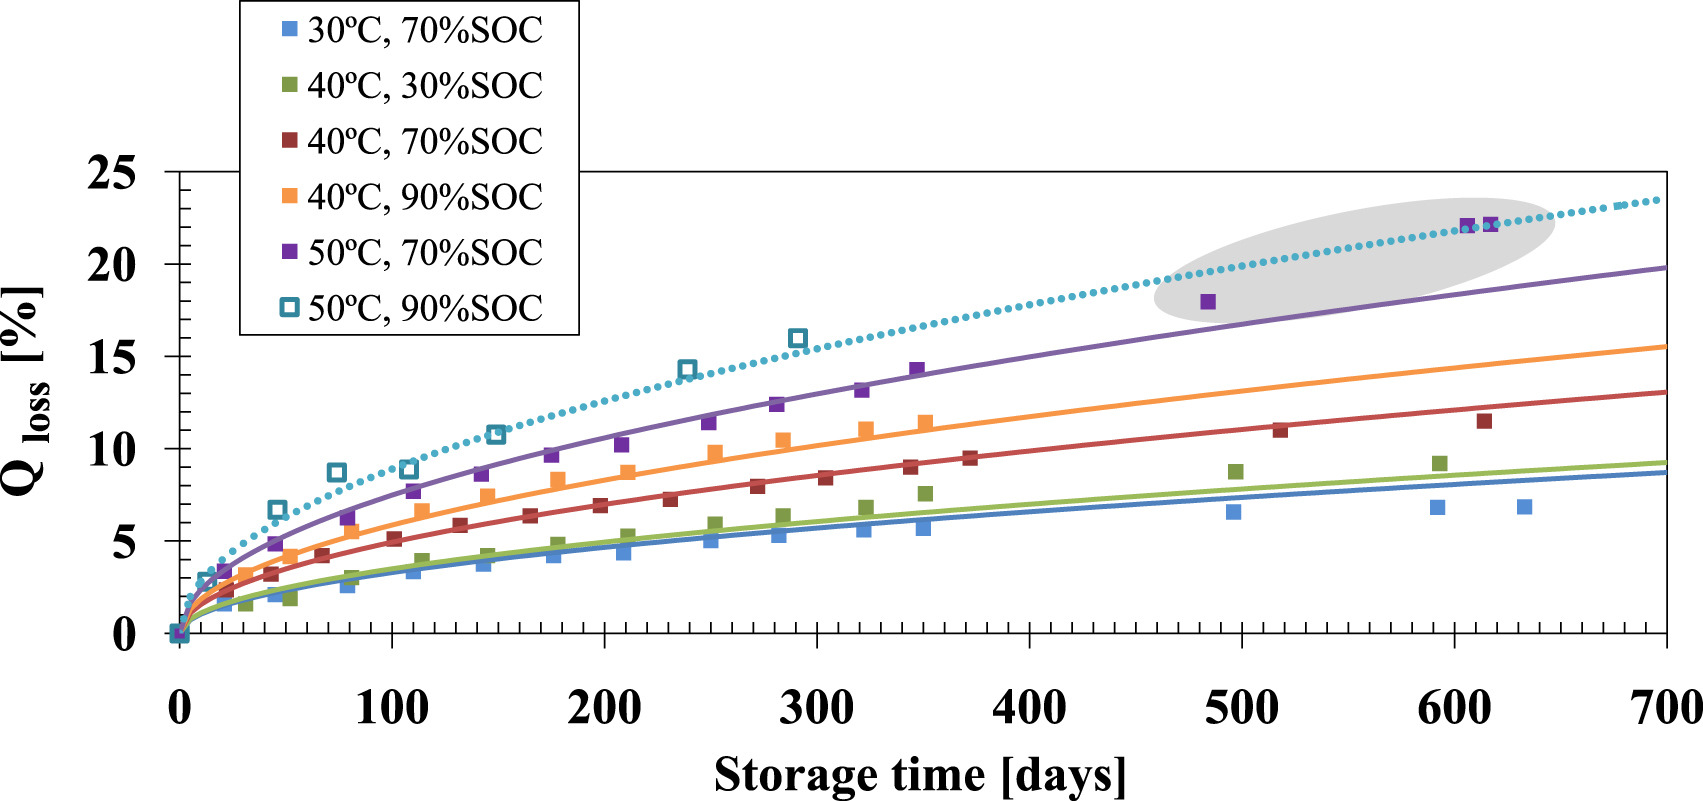
\includegraphics[width=\textwidth]{Figures/05Theory/battery_calendar_aging.jpg}
    \caption[Battery Calendar Aging]{Battery Calendar Aging from \textit{(E. Sarasketa-Zabala et al., 2014 p.53)}\cite{SARASKETAZABALA201445}. The y-axis shows the capacity loss $\mathbf{Q_{loss}}$ as a percentage of the battery capacity.}
    \label{fig:battery_calendar_aging}
\end{figure}

\begin{figure}
    \centering
    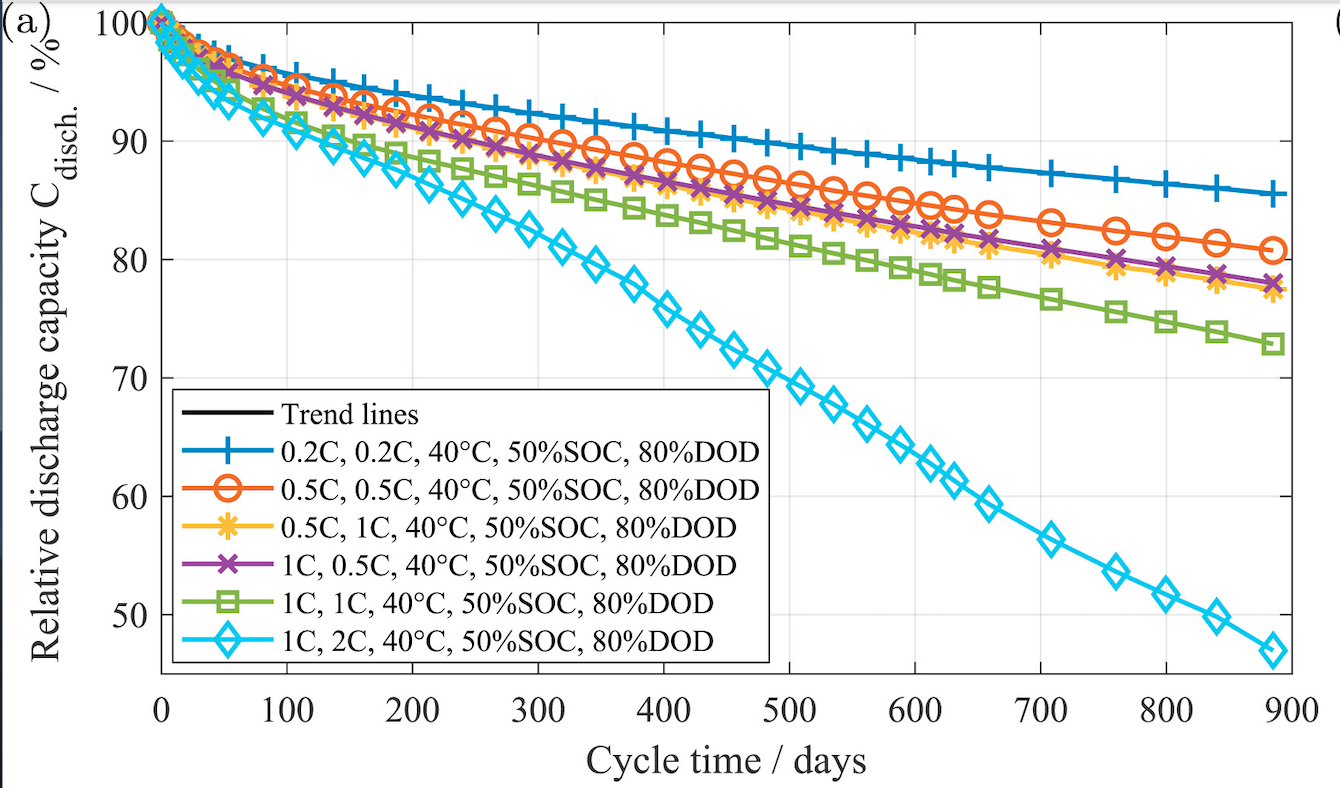
\includegraphics[width=\textwidth]{Figures/05Theory/battery_cycle_aging_cut.png}
    \caption[Battery Cycle Aging]{Battery Cycle Aging from \textit{(M. Naumann et al.,2020 p.6)}\cite{NAUMANN2020227666}.The y-axis shows the relative discharge capacity $\mathbf{C_{disch}}$.}
    \label{fig:battery_cycle_aging_cut}
\end{figure}

The same authors later published two papers considering cycle ageing. In a similar setup, lithium-ion batteries were cycled at different DOD, charge/discharge rates around different SOC points. All under varying temperatures. The results, where the ones from \textit{(M. Naumann et al.,2020)} is shown in \ref{fig:battery_cycle_aging_cut} show that the time-wise decrease in the discharge capacity is greater at high charge/discharge rates when the other conditions are kept equal. The best result in terms of time-wise degradation was in their results at 0.2C.\cite{SARASKETAZABALA2015573}\cite{NAUMANN2020227666}. 

The studies into battery cycle and calendar ageing therefore suggest that the control system should aim to 
\begin{itemize}
    \item \textit{Keep charge/discharge low}    -   Limit the current in and out of the battery to limit cycle ageing. Preferably at no higher than 0.2C.
    \item \textit{Avoid potentiostatic hold at high SOC}    -   When the battery is not used, it should not rest at a high SOC because of the effect on calendar ageing. 
\end{itemize}
\cleardoublepage

\chapter{System Overview}
\label{chap:system_overview}
\section{System overview}
DCP operates more than a hundred sites across the developing world. The sites serve different needs and hence have different-sized equipment. Some of the sites are \textit{islanded} meaning that they do not have a grid connection, while others are connected to a larger grid. Grid-connected sites could feasibly become candidates for a control system in the future. The first pilot however, and hence this thesis, will only consider islanded systems. Specifically, the solution and analysis of this thesis will focus on Chiwoza which is a medium-scale system supporting a health facility in rural Malawi.\\

Chiwoza has a microgrid topology as shown in figure \ref{fig:system_topology}. The individual components are \todo{check break}
\begin{itemize}
    \item \textit{PV-modules}   -   The systems only source of power production through the photovoltaic effect outlined in section \ref{seq:pv_and_irradiance}. The core component of the module is the PV-panel consisting of several smaller PV-cells. As shown in equation \ref{eq:pv_efficency}, the PV-panel has an efficiency $\eta$ based on its area $A$ and test conditions $P_{STC}$ and $G_{STC}$. Several PV-panels may be connected in series as in \ref{fig:pv_serial} adding their voltage and forming a PV-string. Several PV-strings may form a parallel configuration known as a PV-array, shown in \ref{fig:pv_parallel},  adding together their current. Each PV-array has a charge controller controlling the production. Lastly, several PV-arrays may again be connected in parallel to form the PV-module shown in \ref{fig:system_topology}. The goal of the configuration is to achieve the highest power without breaking the constraints set by other equipment such as the charge controller. The PV-modules are ground mounted at an angle, $\rho$, with an orientation described by the azimuth, $\alpha$, determining the amount, type and timing of irradiance reflected onto the modules. These, and the other relevant parameters for the PV-panels at Chiwoza are listed in \autoref{tab:chiwoza_pv_param}.
    
    \item \textit{Charge Controller}   -   Between the PV-array and DC-bus there is the charge controller. The DC-bus requires a certain voltage to charge the battery and connect to the inverter. This may vary somewhat based on the inverter demand and battery state of charge. Furthermore, the power from the PV-array varies with the solar conditions. The charge controller needs to convert the voltage from the PV-panels to the voltage of the DC-bus. A simple charge controller force the PV-array to operate at the DC-bus voltage. As PV-panels have a rated power curve, this is inefficient and leads to large losses of potential power. More modern Maximum Power Point Tracking (MPPT) controllers finds and set the optimum voltage for the PV-array, allowing for the maximal power output. This is then converted into the voltage required for the DC-bus.\cite{Svarc2022-oh} The output from the charge controller will be limited by the maximum allowed voltage on the DC-Bus,$V^{MAX}_DC$, and the maximum current the charge controller can output $I^{MAX}_{CC}$. As mentioned earlier, if there are multiple charge controllers,$n_{CC}$, the currents are added together increasing the total power, $P^{MAX}_{CC}$, from the PV-module. The parameters for the charge controllers  at Chiwoza is listed in \autoref{tab:chiwoza_cc_param}.
    
    \item \textit{Battery module}   -   The battery module stores the power produced by the PV-modules. The batteries used for DCPs systems are mostly \textit{lithium iron phosphate} (LiFePo4) batteries, with a few exceptions using \textit{lead-acid} batteries. Key parameters for the battery is the energy capacity, $E$, which expresses how much charge a battery can deliver at a specific discharge rate at its nominal voltage, and the \textit{min SOC} which describes at which SOC level the battery is no longer supplying. For this thesis, the maximum charge and discharge power,$P_B$ which tells how much current can be continuously delivered at the nominal voltage is also of interest and found for Chiwoza in \autoref{tab:chiwoza_bat_param}.  
    
    \item \textit{DC-Bus}   -   The DC-bus connects the charge controller, the battery and the inverter. Its voltage, shown as $V^{MAX}_{DC}$ in \autoref{tab:chiwoza_cc_param} should remain stable.
    
    \item \textit{DC/AC inverter}   -   The inverter separates the DC and AC sides of the microgrid. It converts the power from the DC side to supply the AC power needed for the loads at the AC side. The inverter has a maximum power limit, $inv_{max}$ constrains the amount of power the DC side can supply. The inverter capacity and efficiency for Chiwoza are found in table \ref{tab:chiwoza_inv_param}. 
    
    \item \textit{Load}   -   The loads are all connected equipment and lighting consuming the power. All loads are on the AC-side of the inverter. The various loads that are connected at Chiwoza is found in \autoref{tab:loads_chiwoza}. These were found through the user survey described in \autoref{seq:user_survey}. There are loads supporting the purpose of the facility at the site, these are known as \textit{Purpose loads}, or in the case of Chiwoza, \textit{Medical Loads}. These include medical equipment, lighting etc. Other loads provides services besides the facility's purpose for staff and visitors at the facility. This might be sockets open for phone charging, cooking appliances etc. There are also other loads that support the facility's purpose indirectly. The water pump and heater are examples of these. \todo{clarify site/facility here}
\end{itemize}
The system installed at the site can be described as a hybrid, islanded microgrid with AC-load. Hybrid because the PV- and battery module can be seen as a hybrid power source. It is important to note that the parameters and models used in this thesis are greatly simplified. 



\begin{figure}
    \centering
    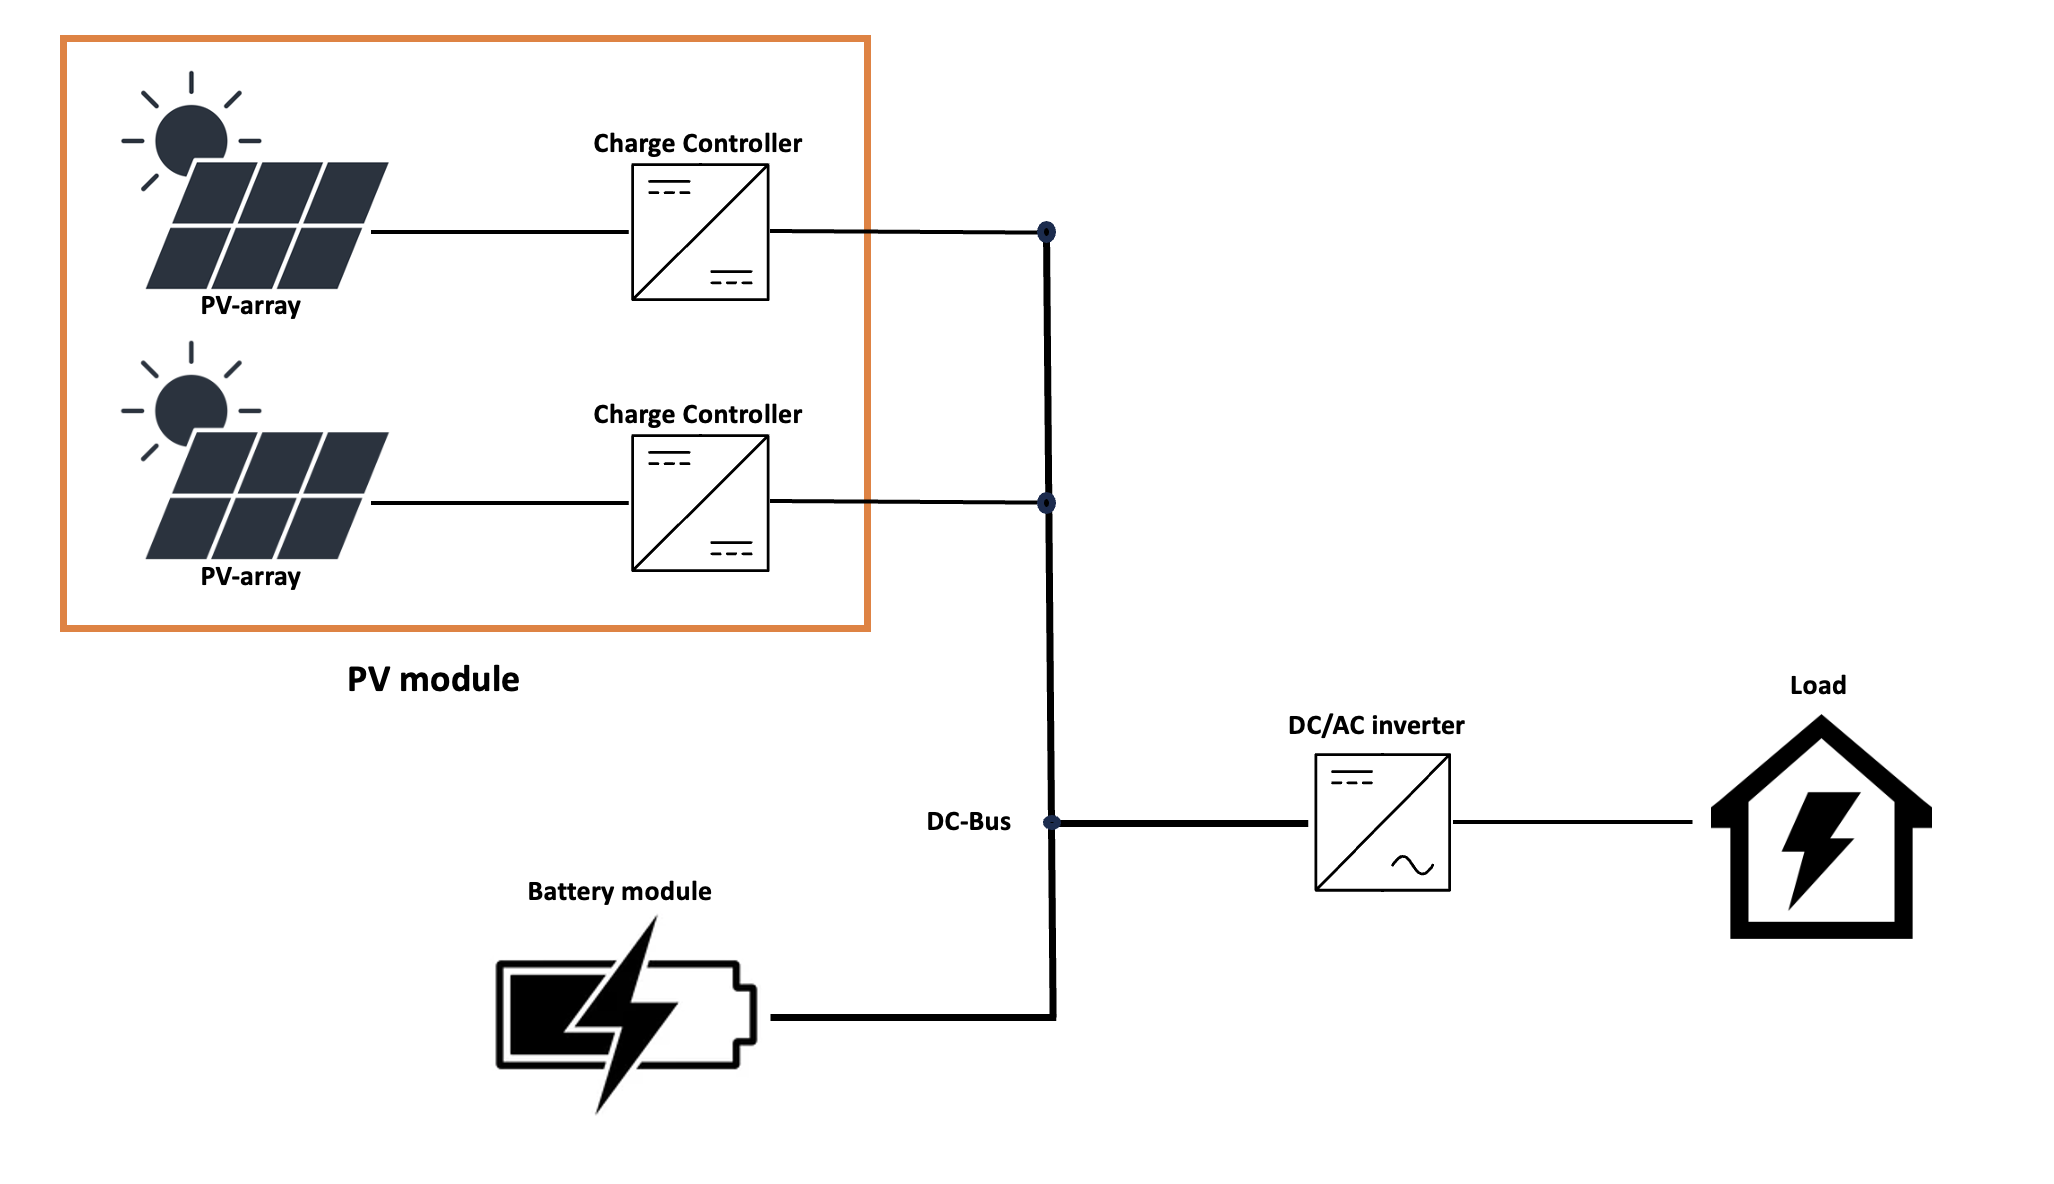
\includegraphics[width=\textwidth]{Figures/06SystemOverview/system_overview.png}
    \caption[Microgrid Topology]{Microgrid topology}
    \label{fig:system_topology}
\end{figure}

\begin{figure}
% First Subfigure
    \begin{subfigure}{\textwidth}
    \centering
    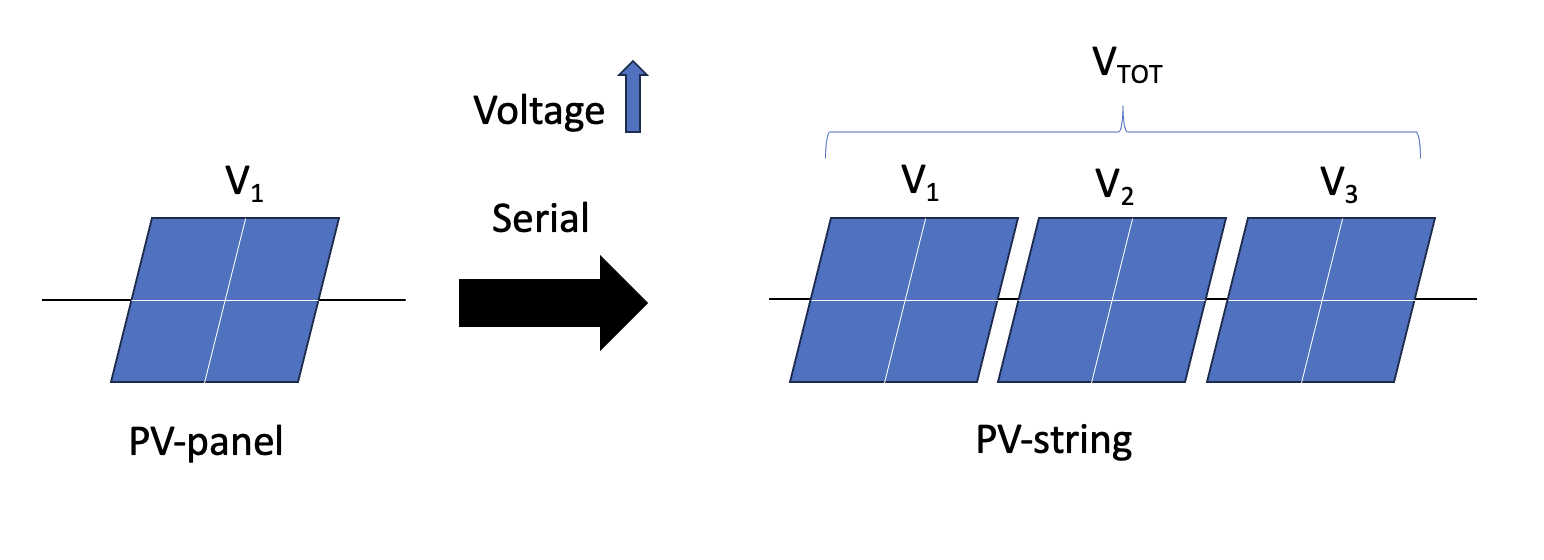
\includegraphics[width=\linewidth]{Figures/06SystemOverview/pv_serial.png}
    \caption[PV-serial]{PV-panels connected in serial forming an PV-string with increased voltage. $V_{TOT} = V_1 + V_2 + V_3$}
    \label{fig:pv_serial}
  \end{subfigure}

  % Add some vertical space between the subfigures
  \vspace{0.5cm}

  % Second Subfigure
  \begin{subfigure}{\textwidth}
    \centering
    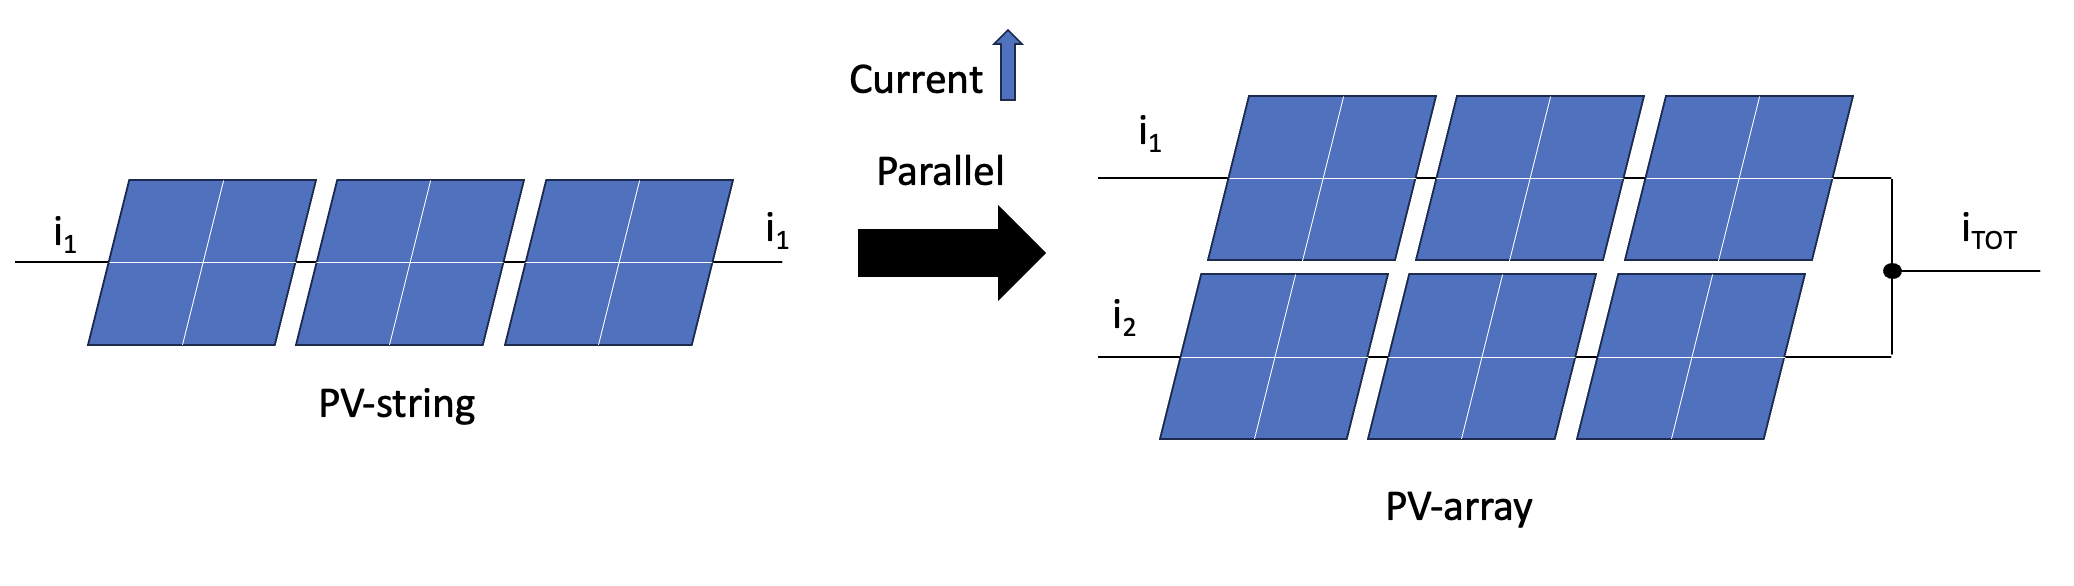
\includegraphics[width=\linewidth]{Figures/06SystemOverview/pv_parallel.png}
    \caption[PV-parallel]{PV-strings connected in parallel forming a PV-array with increased current. $i_{TOT} = i_1 + i_2$}
    \label{fig:pv_parallel}
  \end{subfigure}

  \caption[PV-configuration]{PV-configurations}
  \label{fig:pv_configuration}
\end{figure}

\begin{table}[]
    \centering
    \begin{tabular}{c|c|c|c|c|}
         $P_{STC}[W]$& $G_{STC}[W/m^2]$ & $n_{panels}$& $\rho$ & $\alpha$  \\
         \hline
         375 & 1000 & 25 & 20 & 180  \\
    \end{tabular}
    \caption[Chiwoza PV-parameters]{Chiwoza PV-parameters}
    \label{tab:chiwoza_pv_param}
\end{table}

\begin{table}[]
    \centering
    \begin{tabular}{c|c|c|c|c}
         $V^{MAX}_{DC}[V]$& $I^{MAX}_{CC}[Am]$ & $n_{CC}$ & $P^{MAX}_{CC}[W]$ & Peak Efficiency \\
         \hline
         48 & 60 & 2 & 5760 & 96\%\\
    \end{tabular}
    \caption[Chiwoza Charge Controller parameters]{Chiwoza Charge Controller parameters. The maximum power, $P^{MAX}_{CC}$ is for the two charge controllers combined.}
    \label{tab:chiwoza_cc_param}
\end{table}

\begin{table}[]
    \centering
    \begin{tabular}{c|c|c}
         $E[kWh]$& $P_B,Max[kW]$ &Min SOC\\
         \hline
         7.5 & 7.5 & 5\%\\
    \end{tabular}
    \caption[Chiwoza battery parameters]{Chiwoza battery parameters.}
    \label{tab:chiwoza_bat_param}
\end{table}

\begin{table}[]
    \centering
    \begin{tabular}{c|c}
         $P_{MAX}[kVA]$& Peak Efficiency\\
         \hline
         5 & 99\%\\
    \end{tabular}
    \caption[Chiwoza inverter parameters]{Chiwoza inverter parameters.}
    \label{tab:chiwoza_inv_param}
\end{table}

\begin{table}[ht]
    \centering
    \small % Optional: smaller font size
    \begin{tabularx}{\textwidth}{|X|X|c|}
         \textbf{Load Name} & \textbf{Circuit(s)} & \textbf{Group Abbreviation}\\
         \hline
         Light (Medical) & Medical Light & P1\\
         \hline
         Phone/Laptop Charging (Medical)   &  Staff Socket 3 & P2\\
         \hline
         Oxygen Concentrator & Medical Socket & P3\\
         \hline
         HIV diagnosis equipment & Medical Socket & P3\\
         \hline
         Sterilizer & Medical Socket & P3\\
         \hline
         Microscope & Medical Socket & P3\\
         \hline
         Refrigerator(Medical) & Medical Socket & P5\\
         \hline
         Light (Staff) & Staff Light 1-3, Guardian Shelter Light, Fence Light & S1\\
         \hline
         Phone/Laptop Charging  &  Staff Socket 3, Guardian Shelter Socket  & S2\\
         \hline
         Entertainment (TV,Radio) & Staff Socket 3, Guardian Shelter Socket & S3\\         
         \hline
         Refrigeration (Staff) & Staff Socket 3 & S4\\
         \hline
         Cooking appliances & Staff Socket 3 & S5\\
         \hline
         Water Heater & Water Heater & W1\\
         \hline
         Water Pump & Water Pump & W2\\
         \hline
         $\text{Rental Batteries}^*$ & Rental Battery & H1\\
         \hline
         $\text{Solar Maize Mill}^*$ & Solar Mill & H2
    \end{tabularx}
    \caption[Loads at Chiwoza]{Connected Loads Chiwoza with their circuit and grouping based on \autoref{tab:load_abbreviations}. The loads marked by $*$ are not connected, but planned to be connected as additional revenue-generating loads}
    \label{tab:loads_chiwoza}
\end{table}

\subsection{Measurement and Data logging}\label{seq:data_collection}
Production and load measurement is critical for the effective control and operation of all power systems, including microgrids. All of DCP sites are equipped with several measurement and data logging devices. These may be grouped as in table \ref{tab:measurement_devices}, which shows what each device measures, and what that measurement is used to estimate internally in the device.\\

The measurement from the inverter gives a broad overview of the power flow in the system. On the demand side, this can be further examined by the meters, which are mounted on every circuit. A meter measures the consumption of a load within a time frame. However, as already mentioned, several loads may be connected to the same circuit. The power measurement is only from the circuit, so it is not immediately possible to identify which loads are running based on the consumption measured.\\

Data has been gathered from the site starting from the the installation date of the systems. As the installation date varies between the systems, there are different amounts of historical data for each system. Furthermore, data gathering and operations in developing countries are prone to connectivity issues and tampering with equipment. This has in some instances yielded large gaps or improbable data. There has also been cases of mislabeling of meters, so that meters records consumption for another circuit than the one it is actually to. These issues may be grouped as \textit{data integrity} issues. Low data integrity complicates the analytics and control. Circuits with no recent data in the last 3 months are assumed to be disconnected and hence disregarded in this thesis. This includes Staff Sockets 1 and Staff Sockets 2. 


\begin{table}[h]
    \centering
    \begin{tabular}{c|c|c|c}
        \textbf{Where} & \textbf{Measurement} & \textbf{Estimates} & \textbf{Sample resolution}\\
        \hline
         Battery & Voltage & SOC & minutes\\ 
         \hline
         Smart Meter & Power & Consumption & 15 minutes - 1 hour\\
         \hline 
         Inverter & Power & Production & minutes
    \end{tabular}
    \caption[Measurement devices]{Measurement devices at the sites}
    \label{tab:measurement_devices}
\end{table}


\section{Control System currently in place}\label{seq:current_syst}
As the performance of the proposed solution will be compared against the current control system, an outline of the current control measures is a prerequisite. From the hardware manufacturer, two key control features is included to avoid damage to hardware. These are\todo{check break}
\begin{itemize}
    \item \textit{Inverter overload protection} -   An inverter have a max power capacity. This can be exceeded for a limited amount of time, but if it is exceeded for a prolonged duration, the inverter will shut down to avoid damage. 
    \item \textit{Battery discharge protection} -   As batteries might be damage by a complete discharge due to a high voltage drop, the battery will stop supplying power once it reaches about 5\% State of Charge
\end{itemize}

In addition to this, a battery health measure is implemented by DCP to avoid calendar degradation by prolonged periods at a high state of charge. The control measure, shown as a \textit{Finite State Machine (FSM)} in figure \ref{fig:current_battery_control_FSM}, blocks charging above 90\% SOC early in the day before allowing it to fully charge up during the afternoon. The benefits of this control is consistent with the theory from \ref{seq:battery_health}. The effects of this is shown in figure \ref{fig:battery_charge_control_current}. 

This control measure does not consider future solar production or consumption but is purely a function of the time of day. Similarly, certain high power loads, such as the water pump and water heater are given specific time slots to run, which are all placed during the day when there is normal PV-production. This is however also a purely rule-based control based solely on the time of day.

\begin{figure}[h]
    \centering
    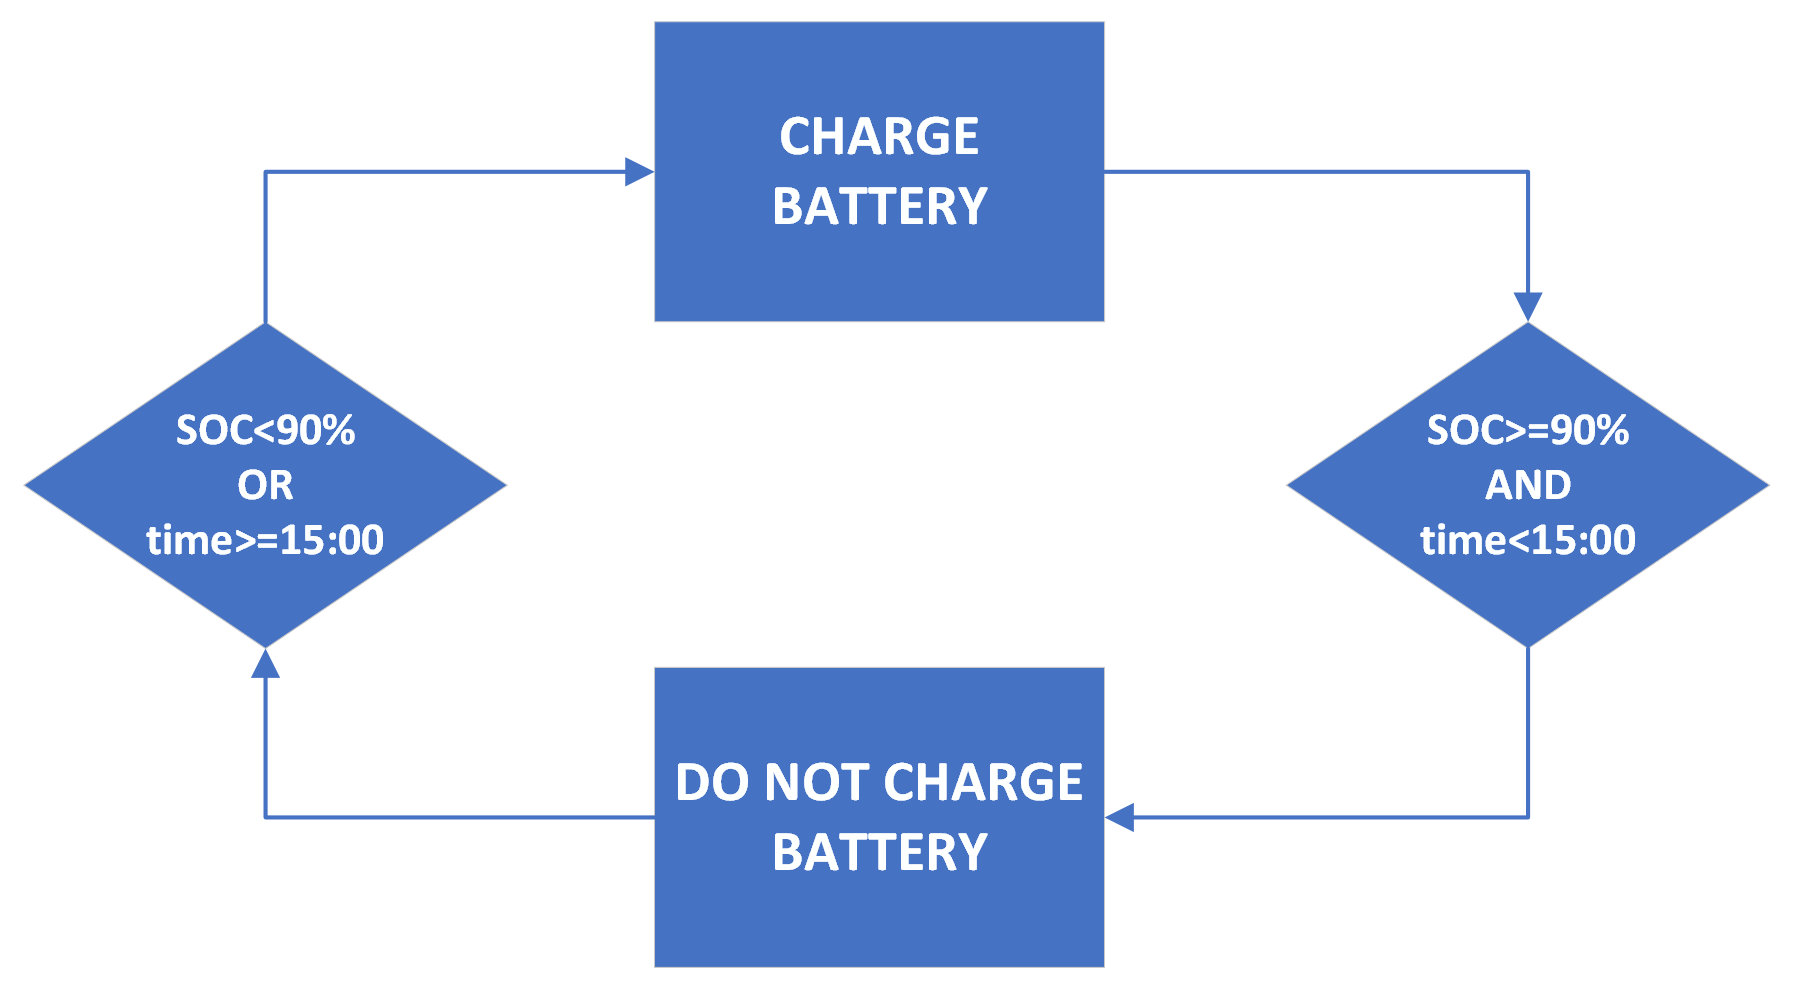
\includegraphics[width=\textwidth]{Figures/06SystemOverview/current_battery_control_FSM.png}
    \caption[Current Battery charge control system FSM]{Battery charge control measure currently in place as a FSM.}
    \label{fig:current_battery_control_FSM}
\end{figure}

\begin{figure}[h]
    \centering
    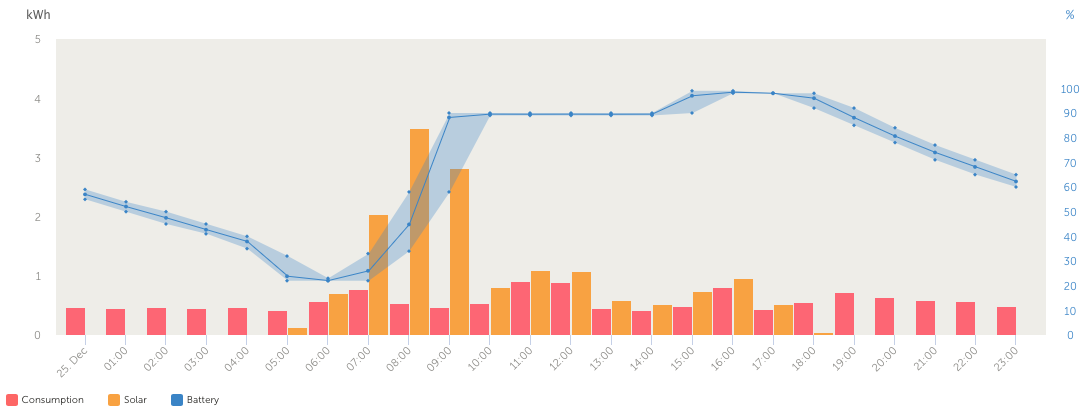
\includegraphics[width=\textwidth]{Figures/06SystemOverview/battery_charge_control_current.png}
    \caption[Current Battery charge control system]{Battery charge control measure currently in place. The picture is taken from DCPs monitoring system showing the operation on December 25th 2023.}
    \label{fig:battery_charge_control_current}
\end{figure}

\subsection{Weaknesses with current control system}\label{sec:weaknesses_current_syst}

\begin{figure}[h]
    \centering
    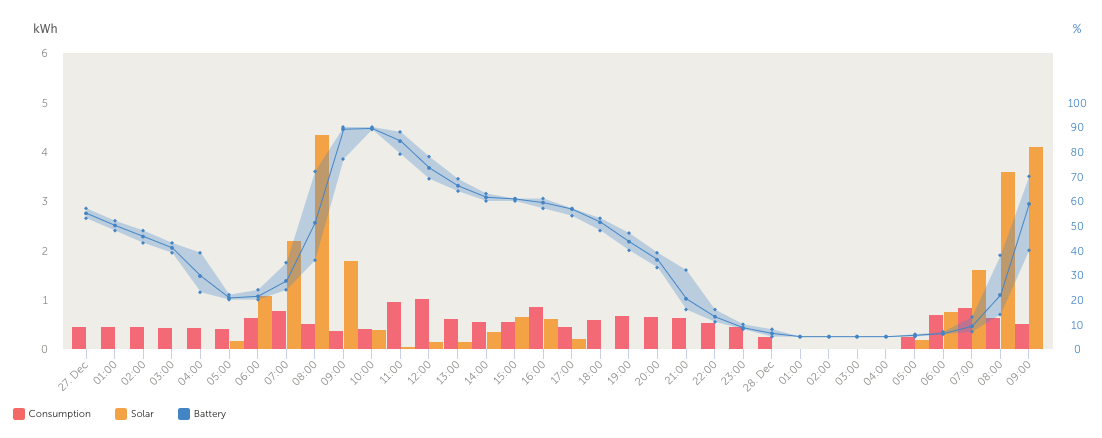
\includegraphics[width=\textwidth]{Figures/06SystemOverview/battery_charge_control_issue.png}
    \caption[Current control system weakness 1 - Battery Depletion]{Screenshot taken from DCPs monitoring platform. The yellow columns shows the production and the red the consumption during each hour. The battery SOC is the blue line.}
    \label{fig:battery_charge_control_issue}
\end{figure}

The two control action taken by DCP regarding the battery charging and time-control of high-power loads are reasonable during normal conditions. The inflexibility with regards to production and consumption conditions however, makes the current control system ill-equipped for days with poor production or high demand. Figure \ref{fig:battery_charge_control_issue} highlights this issue. The battery charge control policy described earlier curtails the charging of the battery after reaching 90\% early in the day, in expectation of being able to charge to remaining part during the afternoon. However, poor production during the afternoon inhibits the charging of the battery. As the battery does not reach its maximum state of charge, it is emptied early during the night. 

At sites with low consumption, there is an opposite problem. In section \ref{seq:battery_health} it was described how cycling the battery at a high state of charge was damaging to the battery. Some sites does not consume more than about 10\% of the battery capacity during nighttime. With the current control system, this will result in a battery cycle between 90-100\% SOC. In figure \ref{fig:battery_issues_high_cycling_chisuwi}, this pattern is shown for the site of Chisuwi, which has a low daily consumption. A more ideal charge cycle would either cycle between two lower values every day, or only charge a few times a week. The two weaknesses of the current control system can be summarized as an inability to adapt to changing conditions and different sites.

\begin{figure}[h]
    \centering
    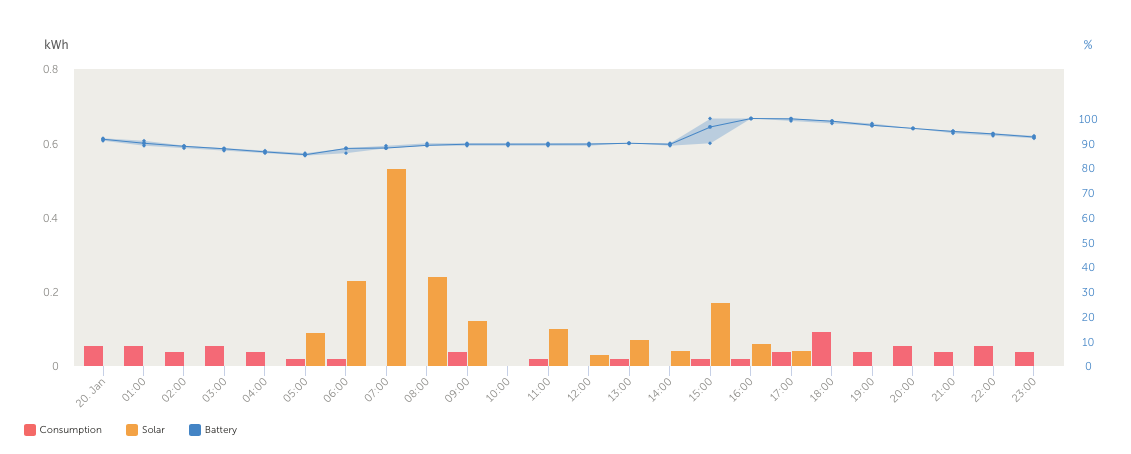
\includegraphics[width=\textwidth]{Figures/06SystemOverview/battery_issues_high_cycling_chisuwi.png}
    \caption[Current control system weakness 2 - High SOC cycling]{Screenshot taken from DCPs monitoring platform. The yellow columns shows the production and the red the consumption during each hour. The battery SOC is the blue line.}
    \label{fig:battery_issues_high_cycling_chisuwi}
\end{figure}

\cleardoublepage

\chapter{Design}
\label{chap:design}
\section{Specification}\label{seq:specification}
The goal of the thesis is to design, propose and evaluate a new control system for the site of Chiwoza. The goal of this section is to specify the stakeholder and criteria of evaluation for such a control system. 

The control system performance is evaluated on a set of key performance indicators (KPIs). The scoring of the control system on these is compared against the current control system. This will form the quantitative basis for the evaluation of the control system.

The KPIs were developed through a thorough process considering all of the stakeholders connected to a system. These stakeholders, listed in table \ref{tab:stakeholders}, have different interests and considerations, this is reflected in the KPIs shown in table \ref{tab:KPI}. 

%Two key concepts of the KPIs is the difference between \textit{demand satisfaction} and \textit{load availability}, and \textit{window of operation}. A demand is satisfied if the load generating the demand is given the required power to run, and the power is consumed. On the other hand, a load can be allocated an amount of power, but not consuming it. This becomes relevant when one wants to save battery power to be able to run certain loads during the night in case of an emergency. 

\begin{table}[h]
    \centering
    \begin{tabular}{|p{3cm}|p{5cm}|p{2cm}|p{5cm}|}
        \hline
        \textbf{Stakeholder} & \textbf{Description} & \textbf{Examples} & \textbf{Main interests} \\
        \hline
        End-user & The final users of the appliances powered by the solar systems & Staff, family of staff, patients etc. & The availability of load on demand \\
        \hline
        Customer & The contract partner paying for the installation and monitoring of the systems & UNICEF, USAID, NCA, WFP & The impact per investment of the systems \\
        \hline
        Provider & The contract partner delivering and monitoring the systems & DCP & The lifetime of the components and the parameters agreed upon in the contract \\
        \hline
    \end{tabular}
    \caption[Stakeholders]{Stakeholders and their main interests}
    \label{tab:stakeholders}
\end{table}

\begin{table}[h]
    \centering
    \begin{tabular}{|p{0.5cm}|p{2.5cm}|p{3cm}|p{4cm}|p{2.2cm}|p{2cm}|}
        \hline
        \#&\textbf{KPI} & \textbf{Description} & \textbf{Motivation} & \textbf{Value} & \textbf{Main Stakeholder} \\
        \hline
        I&Battery Charge/discharge rate & The rate of charge and discharge amount from/to the battery  & The charge/discharge rate is inversely proportional to the battery life & Should not exceed 0.2C & Provider \\
        \hline
        II&Battery SOC & The energy stored in the battery & A high SOC for a prolonged period can damage the battery lifetime  & Should not exceed 90\% SOC & Provider \\
        \hline
        III&User satisfaction & The ability to satisfy a load demand weighted by the user importance of the load.  & The end-users have placed different importance to the various loads.  & $\mathbf{R}^+$ & End-user  \\
        \hline
        IV&Utilization & The ratio between utilized and potential solar production & The Customer would like to see that the systems they have procured is used  & 0-100\% & Customer \\
        \hline
        V&Critical Load Reliability & Reliability for critical loads as described in section \ref{sec:reliability}. & To showcase the ability to supply power for the facility's purpose & 0-100\% & Customer \\
        \hline
    \end{tabular}
    \caption[KPIs]{KPIs}
    \label{tab:KPI}
\end{table}

\begin{table}[ht]
    \centering
    \begin{tabular}{|c|p{12cm}|}
        \hline
        \textbf{Item} & \textbf{Description} \\
        \hline
        1 & \textbf{Make use of historic data} - As DCP is gathering data from all sites, the control system should use the historic data to guide future behaviour. To not use the available historical data would be to waste an available resource.  The current control system uses no historical data, a new control system that performs worse than the current control system, while using historical data, is therefore to be deemed unsuccessful. \\
        \hline
        2 & \textbf{Continuously control while receiving data sporadically} - The data is gathered at a slower pace than the inherent dynamics of the system. The control system must be able to handle this. \\
        \hline
        3 & \textbf{Adjustable to changing goal prioritization} - The system must be able to adjust to different prioritizations of goals. The ability to do so should be visible in the results. \\
        \hline
        4 & \textbf{Adaptive to changing conditions} - Conditions such as production and consumption might change a lot during the system operation. Sometimes there will be no forecast warning of this. The control system should then quickly react and adapt. \\
        \hline
        5 & \textbf{Be applicable across multiple sites} - As DCP runs several sites, the control system cannot be only tailored to an individual site but needs to be modifiable to serve several similar ones. \\
        \hline
    \end{tabular}
    \caption{Control System Specifications}
    \label{tab:control_system_specification}
\end{table}

The designed control system should also satisfy the set of specifications listed in table \ref{tab:control_system_specification}. These does not assert the control system performance but offer a basis to qualitatively evaluate the proposed system.\\

%\begin{enumerate}
%    \item \textbf{Make use of historic data}    -   As DCP is gathering data from all sites, the control system should use the historic data to guide future behaviour. The current control system use no historical data, a new control system that performs worse than the current is therefore to be deemed unsuccessful.
 %   \item \textbf{Continuously control while receiving data sporadically}   -   The data is gathered at a slower pace than the inherent dynamics of the system. The control system must be able to handle this.
  %  \item \textbf{Adjustable to changing goal prioritization}   -   The system must be able to adjust to different prioritizations of goals. The ability to do so should be visible in the results.
   % \item \textbf{Adaptive to changing conditions}   -   Conditions such as production and consumption might change a lot during the system operation. Sometimes there will be no forecast warning of this. The control system should then quickly react and adapt.
    %\item \textbf{Be applicable across multiple sites}  -   As DCP runs several sites, the control system cannot be only tailored to an individual site but needs to be modifiable to serve several similar ones. 
%\end{enumerate}

To suit the specifications, a control system with the components as shown in figure \ref{fig:control_syst} should be constructed. The individual role of the components is:
\begin{itemize}
    \item \textit{Forecaster}   -   Make use of historical data and measurements to provide a load and production forecast to the optimizer. Must be able to update its forecasts based upon new measurements.
    \item \textit{Optimizer}    -   Make use of the forecast data to provide an optimal plan to the controller.
    \item \textit{Controller}   -   Using the plan from the optimizer, allow or disallow the running of loads and provide charge to the battery.
\end{itemize}

The design of these components will be detailed in the subsequent sub-chapters while the implementation in a simulated environment is found in the following chapter.

\begin{figure}
    \centering
    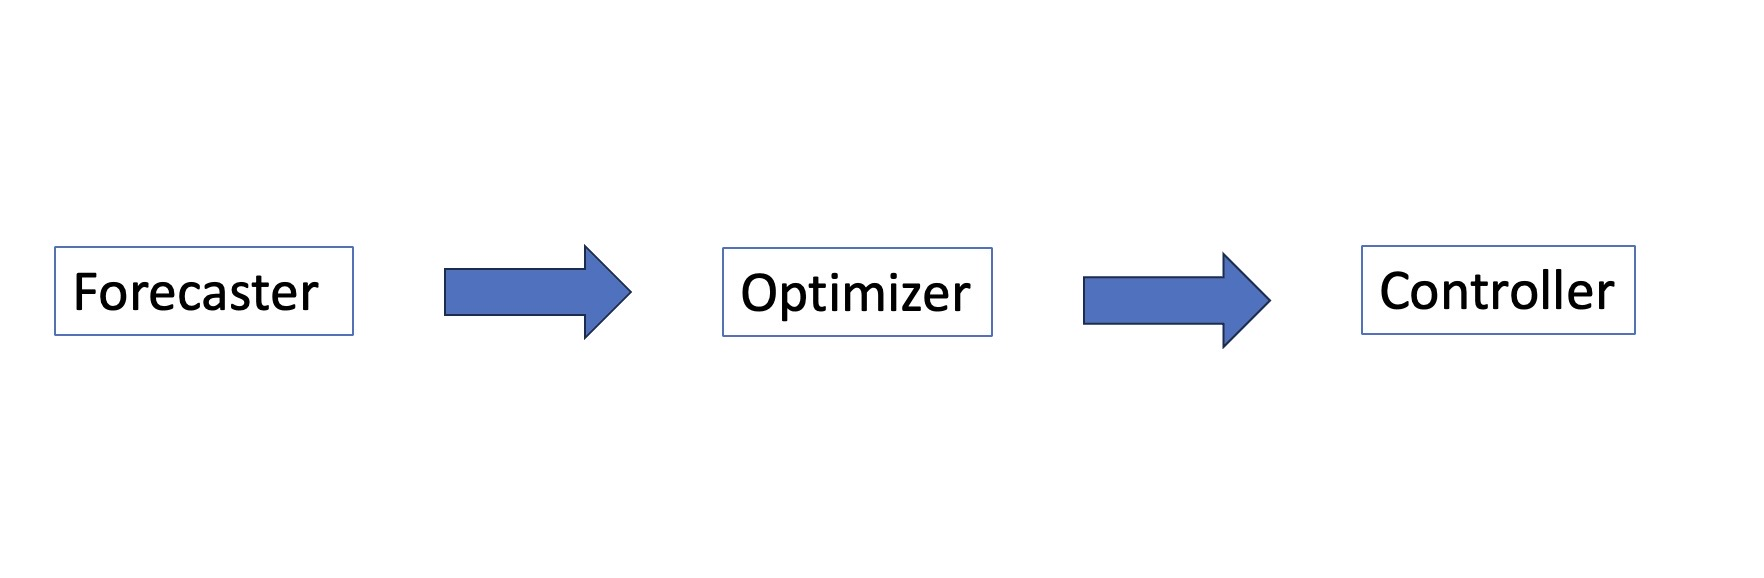
\includegraphics[width=\textwidth]{Figures/06Design/control_overview.jpg}
    \caption[Control system components]{Control system components}
    \label{fig:control_syst}
\end{figure}


\section{Load analysis}

Chiwoza is, as shown in figure \ref{fig:system_topology}, solely powered a hybrid source consisting of a battery and PV-module. As solar power is an intermittent and \textit{non-dispatchable} resource, the only control levers are the power to and from the battery and the enabling/disabling of loads. To control a system by adjusting the load is known as \textit{demand-side-management}(DSM). For a DSM-control system to be effective, a thorough and accurate understanding of the connected loads is necessary. This is gained through load analysis. There are 3 main goals to be achieved from this process:
\begin{enumerate}
    \item \textbf{Understand consumption pattern}    - The total demand varies both in how much power is demanded, and when it is demanded. This is also true on the disaggregated level for the consumption for each load. This creates a consumption pattern across time. When attempting to control the consumption, the goal is to predict the pattern into the future. This will is the subject of the next section \ref{seq:load_forecasting} on load forecasting. A prerequisite for the work in that section is an understanding of the historical consumption pattern.
    \item \textbf{Understand load value}    -   As loads vary in their purpose, the end users will value the available loads differently. This valuation is unlikely to be static but will vary based on circumstances such as the time of day. The control system will prioritize certain loads over other. This prioritization should be partly based on how the end-users value the loads present at the site. The information about valuation is gained through a user survey described in section \ref{seq:user_survey}.
    \item \textbf{Classifying types of loads}   -   Loads also differ in other aspects, such as the flexibility of demand. Certain loads need to satisfy an immediate goal, while others are more flexible in when demand can be met. Understanding this difference between the loads are fundamental for identifying the available control options. This work is done in section \ref{seq:load_classification}.
\end{enumerate}

For this thesis, the load analysis was performed through the gathering of transmitted data and user queries. The available data from the monitoring system detailed in subsection \ref{seq:data_collection}. The most important being the time-series showing the disaggregated-by-meter and total consumption.\\

\subsection{Statistical analysis}

The statistical load analysis attempts to draw conclusion based on historic data. Starting out by considering the total daily consumption, plotted from October 23rd to December 23rd 2023 in \ref{fig:tot_con_daily_chiwoza_20231023-1223}  seems to vary around a mean. At the the 20th of December, there seems to be a significant drop in consumption. This could be reflect an actual lower consumption, a problem with the data or a failure of the system.\\ 

It is also possible to examine consumption at a higher time-resolution, down to the hourly level. Figure \ref{fig:tot_con48_chiwoza_202310} shows the consumption in October 2023 plotted as successive 48 hour periods. Each gray line represent a 48 hour period. These are mostly centered around the average, shown in blue. It is clear that for total consumption, the variance within a day is much larger than the variance between days. There are certain spikes indicating a sudden large, but short-lasting consumption during the daytime. The section \ref{seq:current_syst} on current control measures states that certain high power loads are set to run only at specific time intervals during the day. This pattern is likely a cause of that.\\

\begin{figure}
    \centering
    \includegraphics[width=\textwidth]{Figures/06Design/tot_con_daily_chiwoza_20231023-1223.png}
    \caption[Daily consumption Chiwoza 20231023-1223]{The total daily consumption of Chiwoza from October 23rd to December 23rd 2023. Included with the 5 day average. Weekends are shaded in grey.}
    \label{fig:tot_con_daily_chiwoza_20231023-1223}
\end{figure}

\begin{figure}
    \centering
    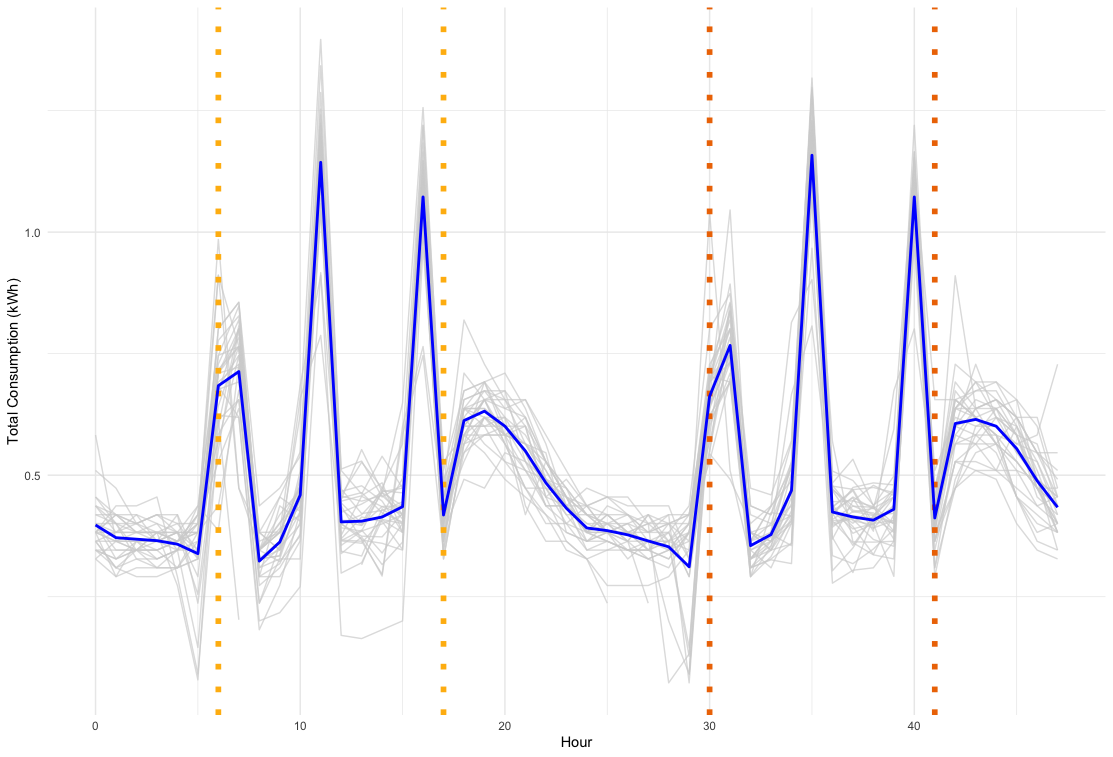
\includegraphics[width=\textwidth]{Figures/06Design/tot_con48_chiwoza_202310.png}
    \caption[Consumption Chiwoza October successive 48h-periods]{The total consumption of Chiwoza for successive 48-hour periods starting at midnight over the month of October 2023. The average across the month is highlighted in blue, and the start and end of normal daylight time is indicated by the doted lines for the two days respectively. The spikes in the pattern is due to time-regulated usage of a heavy use water pump.}
    \label{fig:tot_con48_chiwoza_202310}
\end{figure}

The total consumption of a site may be split into the consumption measured by the meters mounted at the various circuits. This yields an disaggregated view of the consumption based on the specific usage. As outlined in section \ref{seq:data_collection}, this is the highest level of resolution of which to analyse historical consumption data on. In figure \ref{fig:con_disagg_chiwoza_20230603-05} the consumption of Chiwoza over a 48 hour period in June 2023 is disaggregated based on meter. This plot supports the proposal in the previous paragraph, that the spikes in consumption was caused by time controlled high-powered loads. The fact that these loads are already controlled, suggest that these are flexible. This means that their past pattern is less interesting, because the pattern can be adjusted as need be. For the other loads, the pattern is important as it is inflexible. Neglecting the flexible loads, the consumption seems to be dominated by the Medical Light and Staff Socket consumption. For the Medical Light not surprisingly there is a increase in consumption during nighttime. This creates a repeating pattern each day. Repeating patterns over a period is known as periodicity, which is a key characteristic to identify for a load. We can be confident that most loads will have periodicity within a day. In addition, some loads might exhibit patterns between days. Identifying these will greatly improve the foundation for forecasting.\\ 

\begin{figure}
    \centering
    \includegraphics[width=\textwidth]{Figures/06Design/con_disagg_chiwoza_20230603-05.png}
    \caption[Disaggregated Consumption Chiwoza 20230603-05]{The disaggregated consumption of Chiwoza over a 48 hour period starting from midnight 2023-06-03. As opposed to the rest of the thesis, the date was selected so far back because afterwards a communication problem with meter on the water heater occurred. In later analysis, loads such as Staff Sockets 1 and 2 have recorded no consumption. }
    \label{fig:con_disagg_chiwoza_20230603-05}
\end{figure}

\subsubsection{Patterns between days}\label{seq:periodicity}

A natural first assumption is that some loads will show a difference consumption between workdays and weekends. Despite being a health facility, where medical emergencies might suddenly require attention, Chiwoza follows a regular Malawian workweek from Monday to Friday. Looking first at the total consumption, the weekends are shaded grey in figure \ref{fig:tot_con_daily_chiwoza_20231023-1223} showing the total consumption. From the plot alone, there are no clear difference between weekdays and weekends for the total consumption. The ACF can also be used to indicate a pattern. If the consumption was largely different between weekdays and weekends, this would have shown up in the ACF as high values at lags corresponding to the current day of week. The ACF across the entire period, shown in \ref{fig:con_acf_day_chiwoza_201023-1223}, shows no such pattern. There are no public holidays in Malawi during this period either, so that is no factor. The analysis does therefore not show enough to support a claim that the day of week influences the total consumption significantly. However, there might be such a pattern for certain loads. \\

\begin{figure}
    \centering
    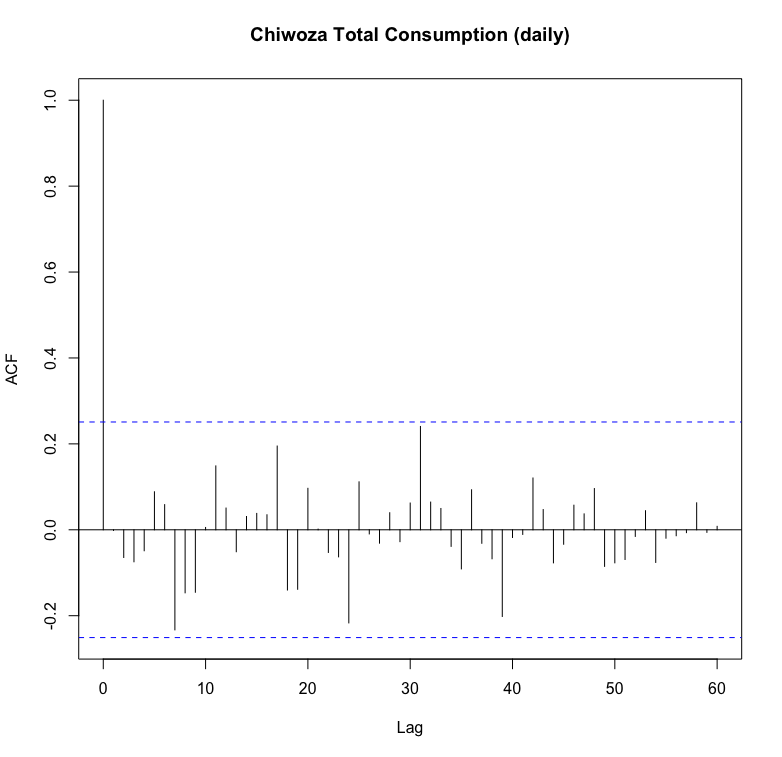
\includegraphics[width=\textwidth]{Figures/06Design/con_acf_day_chiwoza_201023-1223.png}
    \caption[ACF Daily consumption Chiwoza 20231023-1223]{ACF of the total daily consumption at Chiwoza. Lags represents the amount of days back from the December 23rd 2023.}
    \label{fig:con_acf_day_chiwoza_201023-1223}
\end{figure}

The same kind of analysis as performed above can be done on individual loads. The medical light consumption, shown in figure \ref{fig:con_chiwoza_med_light_20231023-1223} have no clear pattern between days. Neither does staff consumption, as seen in figure \ref{fig:con_chiwoza_staff_20231023-1223}. The two loads Medical Sockets and Guardian Shelter Socket, shown in \autoref{fig:con_chiwoza_med_socket_20231023-1223} and \autoref{fig:con_chiwoza_guard_socket_20231023-1223} respectively does however indicate some difference in consumption between weekdays and weekends. The pattern at the Guardian Shelter Socket especially, shows a clear difference, with its consumption happening almost exclusively at weekdays. The ACF across the period for the Guardian shelter supports this as, shown in figure \ref{fig:con_acf_chiwoza_guard_socket_20231023-1223}, the lag representing a 7 days back from December 23rd, a Saturday, is significant. The ACF for the consumption from the Medical Socket, in figure \ref{fig:con_acf_chiwoza_med_socket_20231023-1223} is less clear, with no significant daily lags. This indicates that the difference in consumption between weekdays and weekends are larger for the Sockets at the Guardian Shelter then for the Medical Building. There are also not the same pattern for the light consumption at the guardian shelter, seen in \ref{fig:con_ts_chiwoza_guard_light_202311}, suggesting that the lights are on independently of the day of week. The last load, the fence light shown in figure \ref{fig:con_chiwoza_fence_light_20231023-1223}, have no clear pattern either. The consumption here is also so small, averaging to less than 25Wh a day, so that small deviations have a large effect. \\

\begin{figure}
    \centering
    \includegraphics[width=\textwidth]{Figures/06Design/con_chiwoza_med_light_20231023-1223.png}
    \caption[Medical Light consumption Chiwoza 20231023-1223]{Light consumption in the medical buildings at Chiwoza from October 23rd to December 23rd 2023. 5 day average as dotted line. Weekends shaded in grey.}
    \label{fig:con_chiwoza_med_light_20231023-1223}
\end{figure}

\begin{figure}
    \centering
    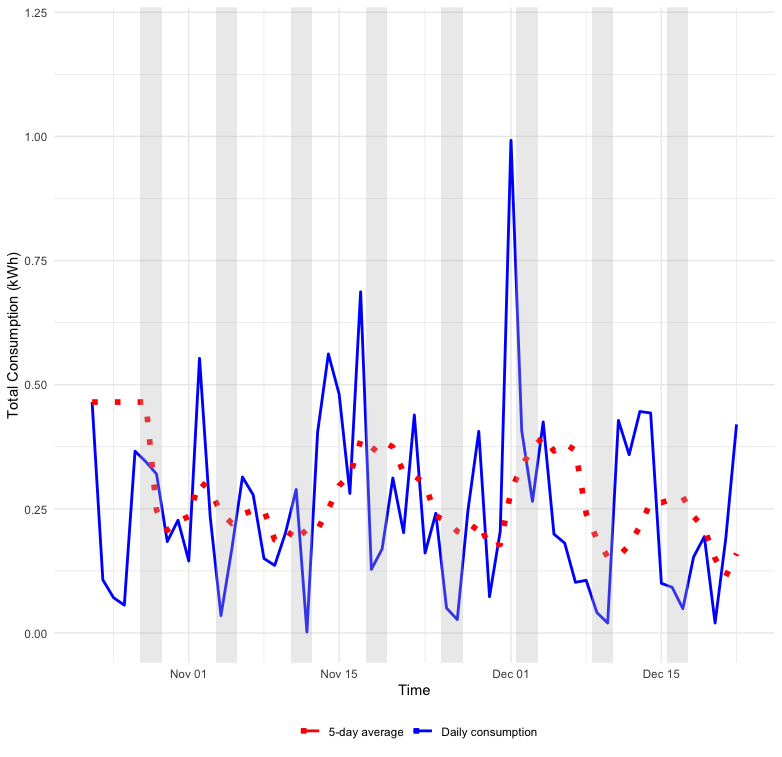
\includegraphics[width=\textwidth]{Figures/06Design/con_chiwoza_med_socket_20231023-1223.png}
    \caption[Medical Socket consumption Chiwoza 20231023-1223]{Consumption from the sockets at the medical building at Chiwoza from October 23rd to December 23rd 2023. 5 day average as dotted line. Weekends shaded in grey.}
    \label{fig:con_chiwoza_med_socket_20231023-1223}
\end{figure}

\begin{figure}
    \centering
    \includegraphics[width=\textwidth]{Figures/06Design/con_chiwoza_guard_socket_20231023-1223.png}
    \caption[Guardina Shelter Socket consumption Chiwoza 20231023-1223]{Consumption from the sockets at the Guardian Shelter at Chiwoza from October 23rd to December 23rd 2023. 5 day average as dotted line. Weekends shaded in grey.}
    \label{fig:con_chiwoza_guard_socket_20231023-1223}
\end{figure}

\begin{figure}
    \centering
    \includegraphics[width=\textwidth]{Figures/06Design/con_chiwoza_guard_light_20231023-1223.png}
    \caption[Guardian Shelter Light consumption Chiwoza 20231023-1223]{Consumption from the Lights at the Guardian Shelter at Chiwoza from October 23rd to December 23rd 2023. 5 day average as dotted line. Weekends shaded in grey.}
    \label{fig:con_chiwoza_guard_light_20231023-1223}
\end{figure}

\begin{figure}
\centering
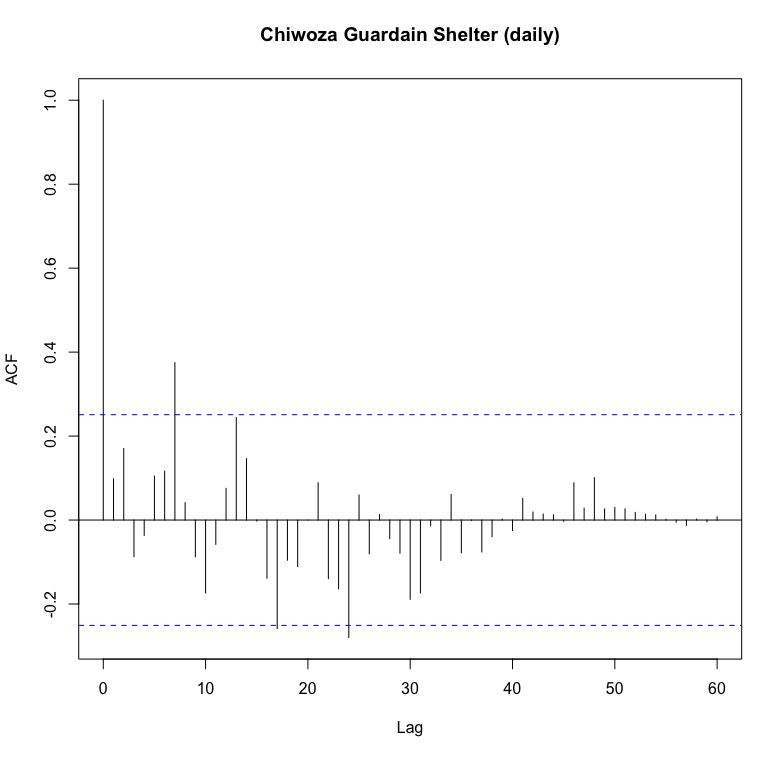
\includegraphics[width=\textwidth]{Figures/06Design/con_acf_chiwoza_guard_socket_20231023-1223.png}
\caption[ACF Guardian shelter socket consumption Chiwoza 20231023-1223]{Auto correlation of consumption measured from the sockets at the Guardian Shelter at Chiwoza between October 23rd to December 23rd 2023. Blue dotted lines represent 95\% confidence interval.}
\label{fig:con_acf_chiwoza_guard_socket_20231023-1223}
\end{figure}

\begin{figure}
\centering
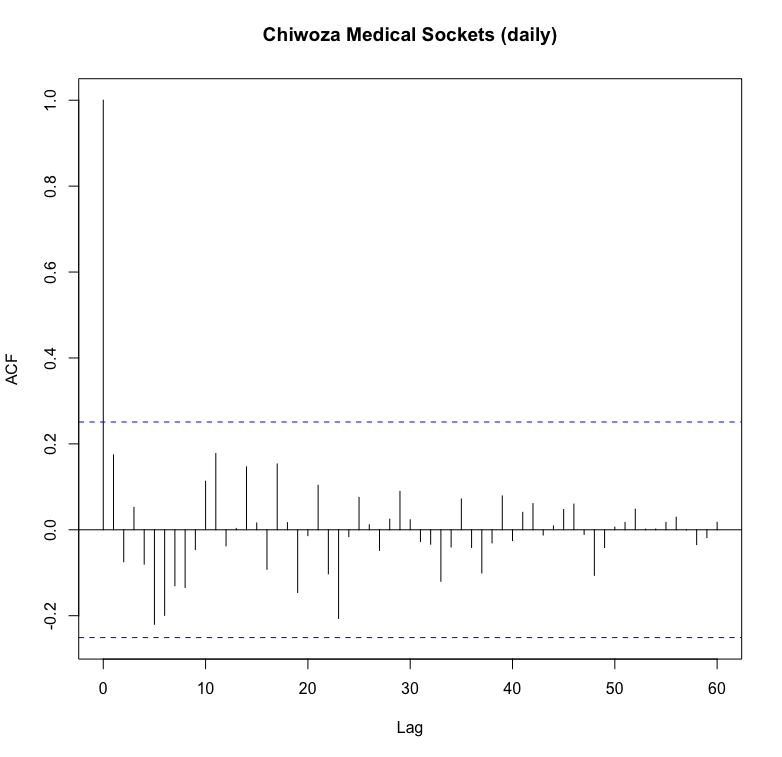
\includegraphics[width=\textwidth]{Figures/06Design/con_acf_chiwoza_med_socket_20231023-1223.png}
\caption[ACF Medical Socket consumption Chiwoza 20231023-1223]{Auto correlation of consumption measured from the sockets at the Medical Building at Chiwoza between October 23rd to December 23rd 2023. Blue dotted lines represent 95\% confidence interval.}
\label{fig:con_acf_chiwoza_med_socket_20231023-1223}
\end{figure}

\begin{figure}
    \centering
    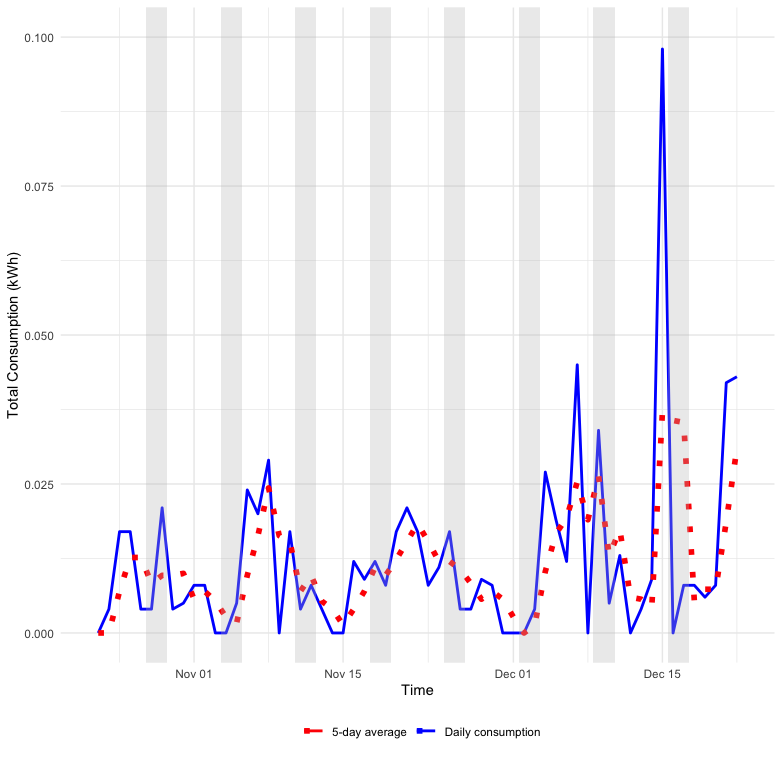
\includegraphics[width=\textwidth]{Figures/06Design/con_chiwoza_fence_light_20231023-1223.png}
    \caption[Fence Light consumption Chiwoza 20231023-1223]{Fence light consumption at Chiwoza from October 23rd to December 23rd 2023. 5 day average as dotted line. Weekends shaded in grey.}
    \label{fig:con_chiwoza_fence_light_20231023-1223}
\end{figure}

\begin{figure}
  \centering
  \begin{minipage}{0.7\textwidth} % Adjust the width as needed
    \centering
    \includegraphics[width=\linewidth]{Figures/06Design/con_chiwoza_staff_light_20231023-1223.png}
    \caption[Staff Light consumption Chiwoza 20231023-1223]{Daily light consumption in the staff buildings at Chiwoza between October 23rd to December 23rd 2023. Weekends shaded in grey.}
    \label{fig:con_chiwoza_staff_light_20231023-1223}
  \end{minipage}

  \vspace{0.5cm} % Add vertical space between the subfigures

  \begin{minipage}{0.7\textwidth} % Adjust the width as needed
    \centering
    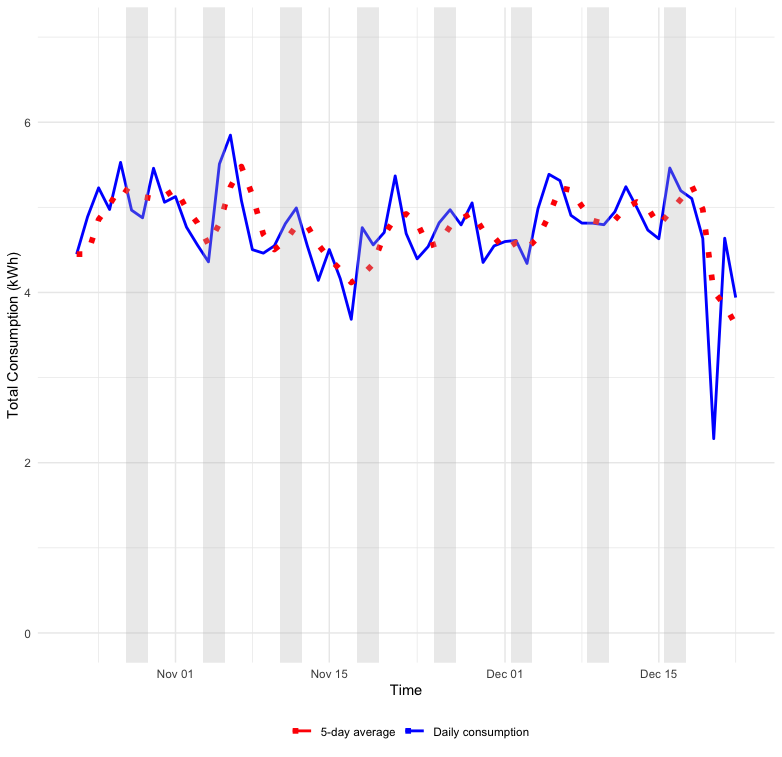
\includegraphics[width=\linewidth]{Figures/06Design/con_chiwoza_staff_socket_20231023-1223.png}
    \caption[Staff Socket consumption Chiwoza 20231023-1223]{Daily consumption measured from the sockets at the staff buildings at Chiwoza between October 23rd to December 23rd 2023. Weekends shaded in grey.}
    \label{fig:con_chiwoza_staff_socket_20231023-1223}
  \end{minipage}

  \caption[Staff consumption Chiwoza 20231023-1223]{Daily consumption at staff buildings in November 2023.}
  \label{fig:con_chiwoza_staff_20231023-1223}
\end{figure}

In summary, the load analysis have identified that apart from the flexible loads, the consumption is dominated by staff and medical usage. These have a clear periodic pattern within a day, but for most of them, no obvious between days. The two exceptions, The Medical Sockets and especially the Guardian Shelter Socket, have a clear enough difference in consumption between the weekdays and weekends to warrant a extra consideration for the forecasting.


\subsection{User survey}\label{seq:user_survey}
A user survey was developed for this thesis in collaboration with DCP. It was performed through phone calls by a local representative to staff members to staff members at the site. A total of 19 sites participated in the survey, all listed in \ref{tab:us_participants}. These vary in size, purpose and location. The goal of the survey was:\todo{check break}
\begin{itemize}
    \item \textit{Map out connected loads}  - Finding which loads are connected to the various sites.
    \item \textit{Discover load prioritization} - Examining how the users value and use the different loads at various times during the day.
    \item \textit{Determining the acceptability for control}    - Determining how able the users are to understand and accept an automatic control system. 
\end{itemize}

In this section, the results relating to loads are discussed. The full results from the questionnaire are included in appendix \ref{appendix:user_survey}. \\

Table \ref{tab:connected_loads} shows the loads reported to be currently connected at the queried sites. When asked to prioritize amongst loads during daytime and nighttime, figure \ref{fig:user_survey_load_daytime_1st&2nd_priority} and \ref{fig:user_survey_load_nighttime_1st&2nd_priority} shows a clear pattern. The users appears on average to value loads related to the purpose of the facility higher than loads related to the leisure of the staff members. This pattern is stronger during the daytime, but even during the night, the first priority is clearly to keep the lights on at the facilities. This is supported by the results in section \ref{seq:forced_choice}, where most respondents answer that they are willing to forgo some days of staff consumption to ensure the availability of facility loads.

\begin{figure}[!h]
  \centering

  % First Subfigure
  \begin{subfigure}{\textwidth}
    \centering
    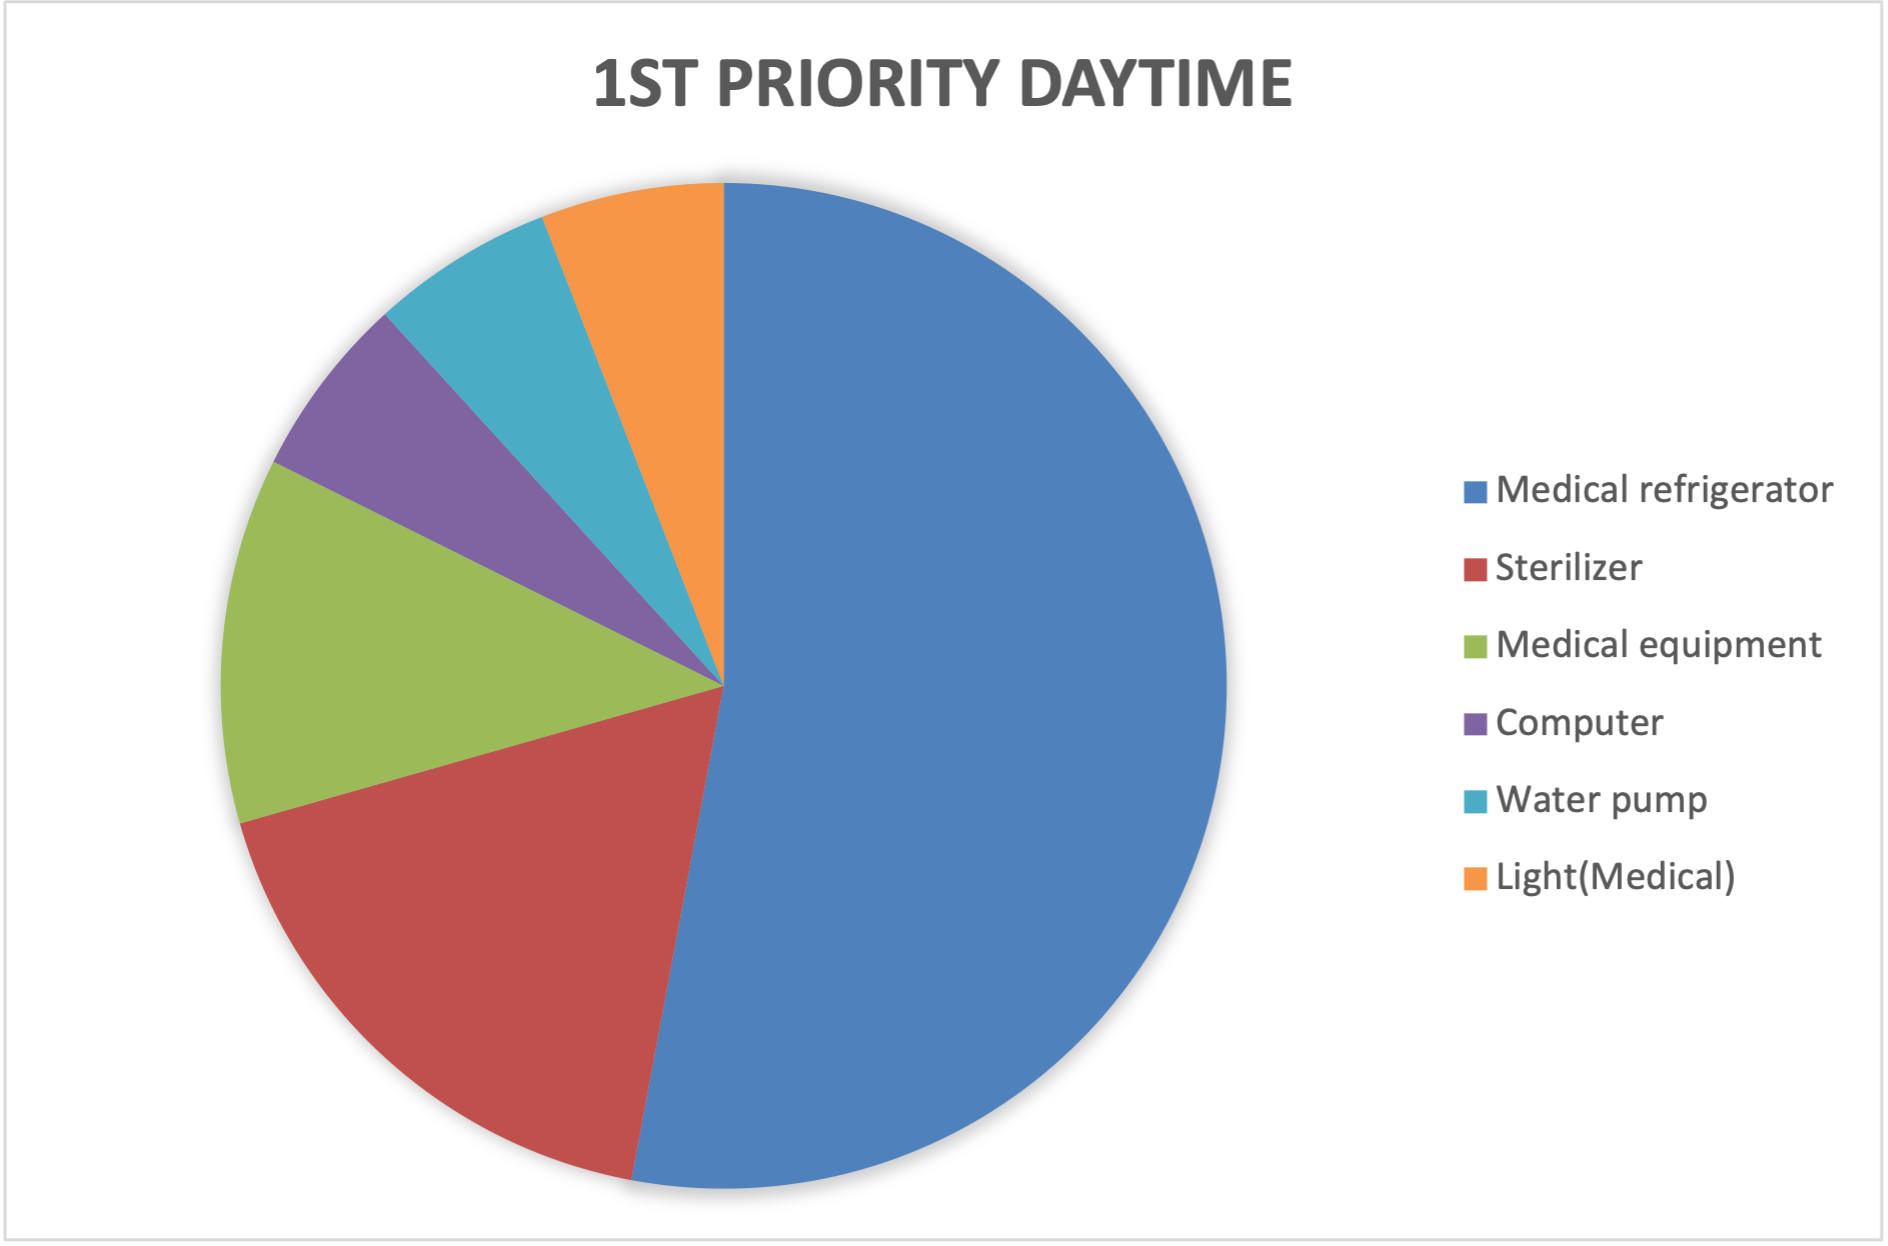
\includegraphics[width=\linewidth]{Figures/06Design/user_survey_load_daytime_1st_priority.png}
    \caption[User survey: Daytime 1st priority]{Reported 1st priority amongst loads during daytime}
    \label{fig:user_survey_load_daytime_1st_priority}
  \end{subfigure}

  % Add some vertical space between the subfigures
  \vspace{0.5cm}

  % Second Subfigure
  \begin{subfigure}{\textwidth}
    \centering
    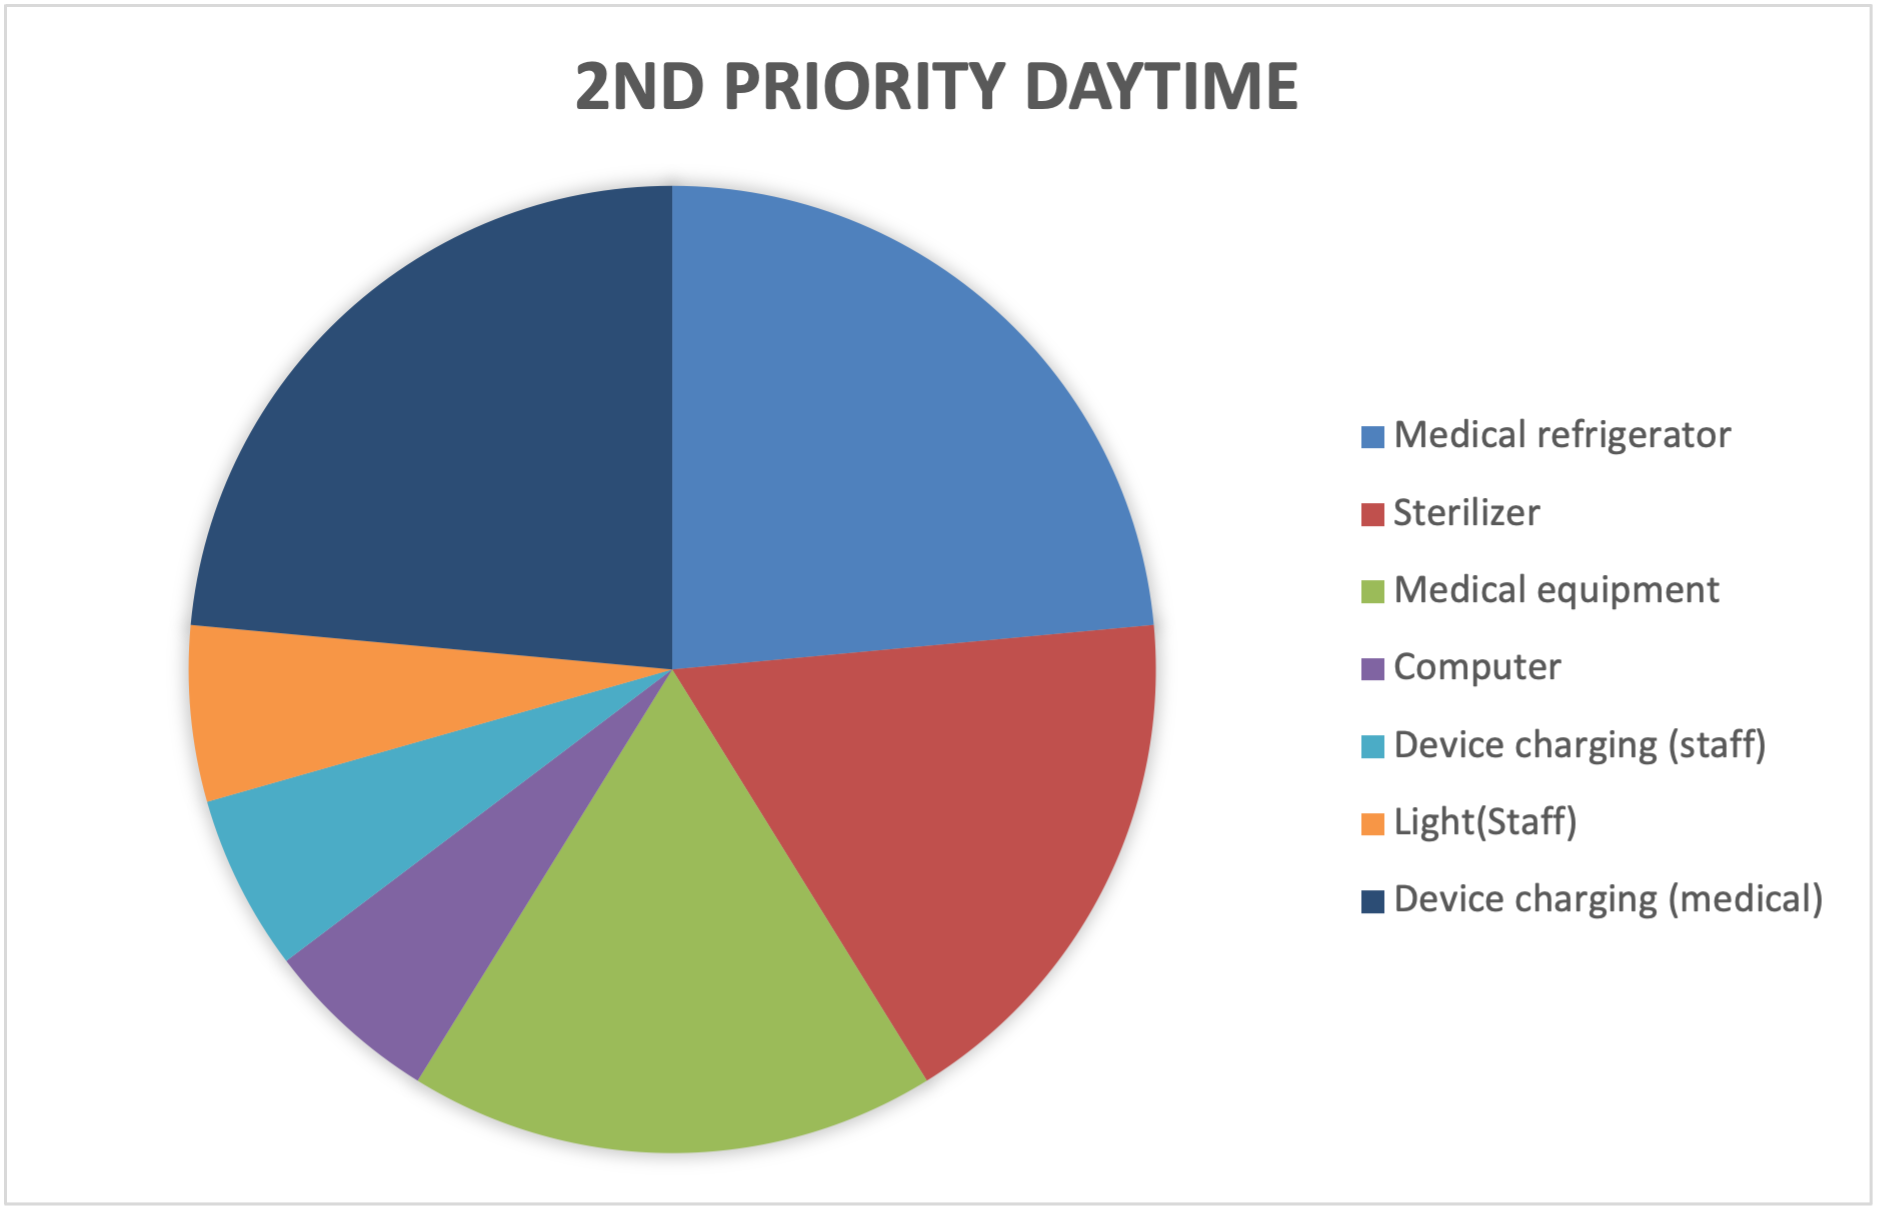
\includegraphics[width=\linewidth]{Figures/06Design/user_survey_load_daytime_2nd_priority.png}
    \caption[User survey: Daytime 2nd priority]{Reported 2nd priority amongst loads during daytime.}
    \label{fig:user_survey_load_daytime_2nd_priority}
  \end{subfigure}

  \caption[User survey: Daytime priority]{Reported 1st and 2nd priority amongst loads during daytime.}
  \label{fig:user_survey_load_daytime_1st&2nd_priority}
\end{figure}


\begin{figure}[!h]
  \centering

  % First Subfigure
  \begin{subfigure}{\textwidth}
    \centering
    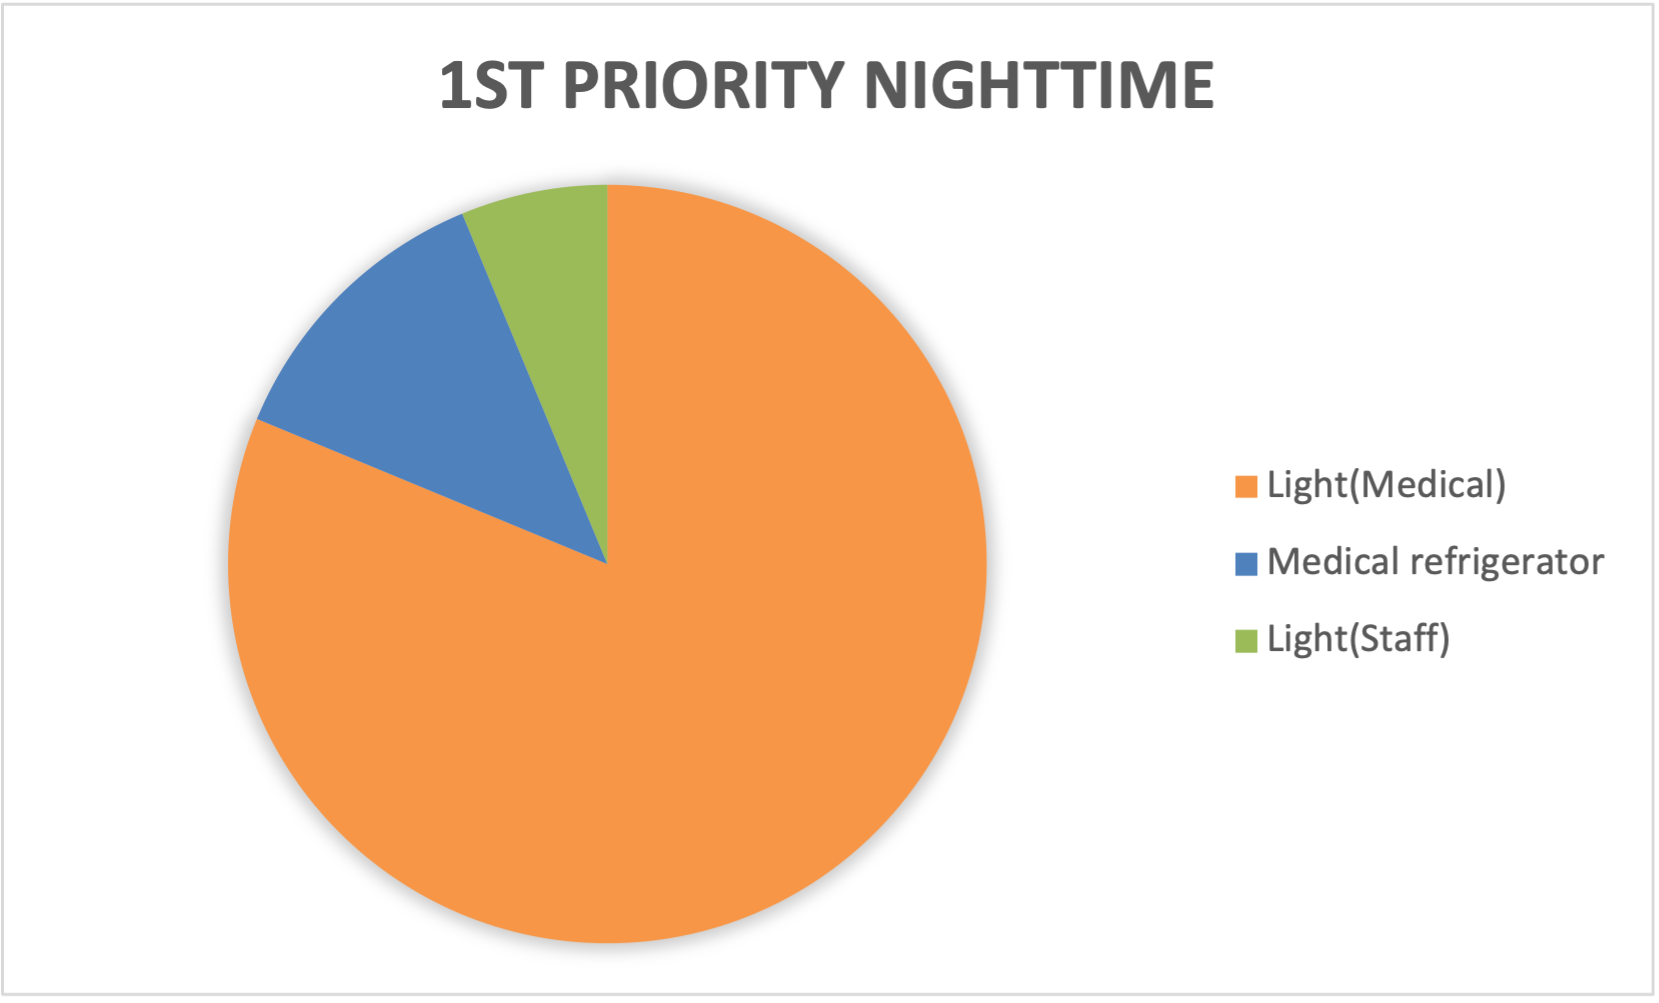
\includegraphics[width=\linewidth]{Figures/06Design/user_survey_load_nighttime_1st_priority.png}
    \caption[User survey: Nighttime 1st priority]{Reported 1st priority amongst loads during nighttime}
    \label{fig:user_survey_load_nighttime_1st_priority}
  \end{subfigure}

  % Add some vertical space between the subfigures
  \vspace{0.5cm}

  % Second Subfigure
  \begin{subfigure}{\textwidth}
    \centering
    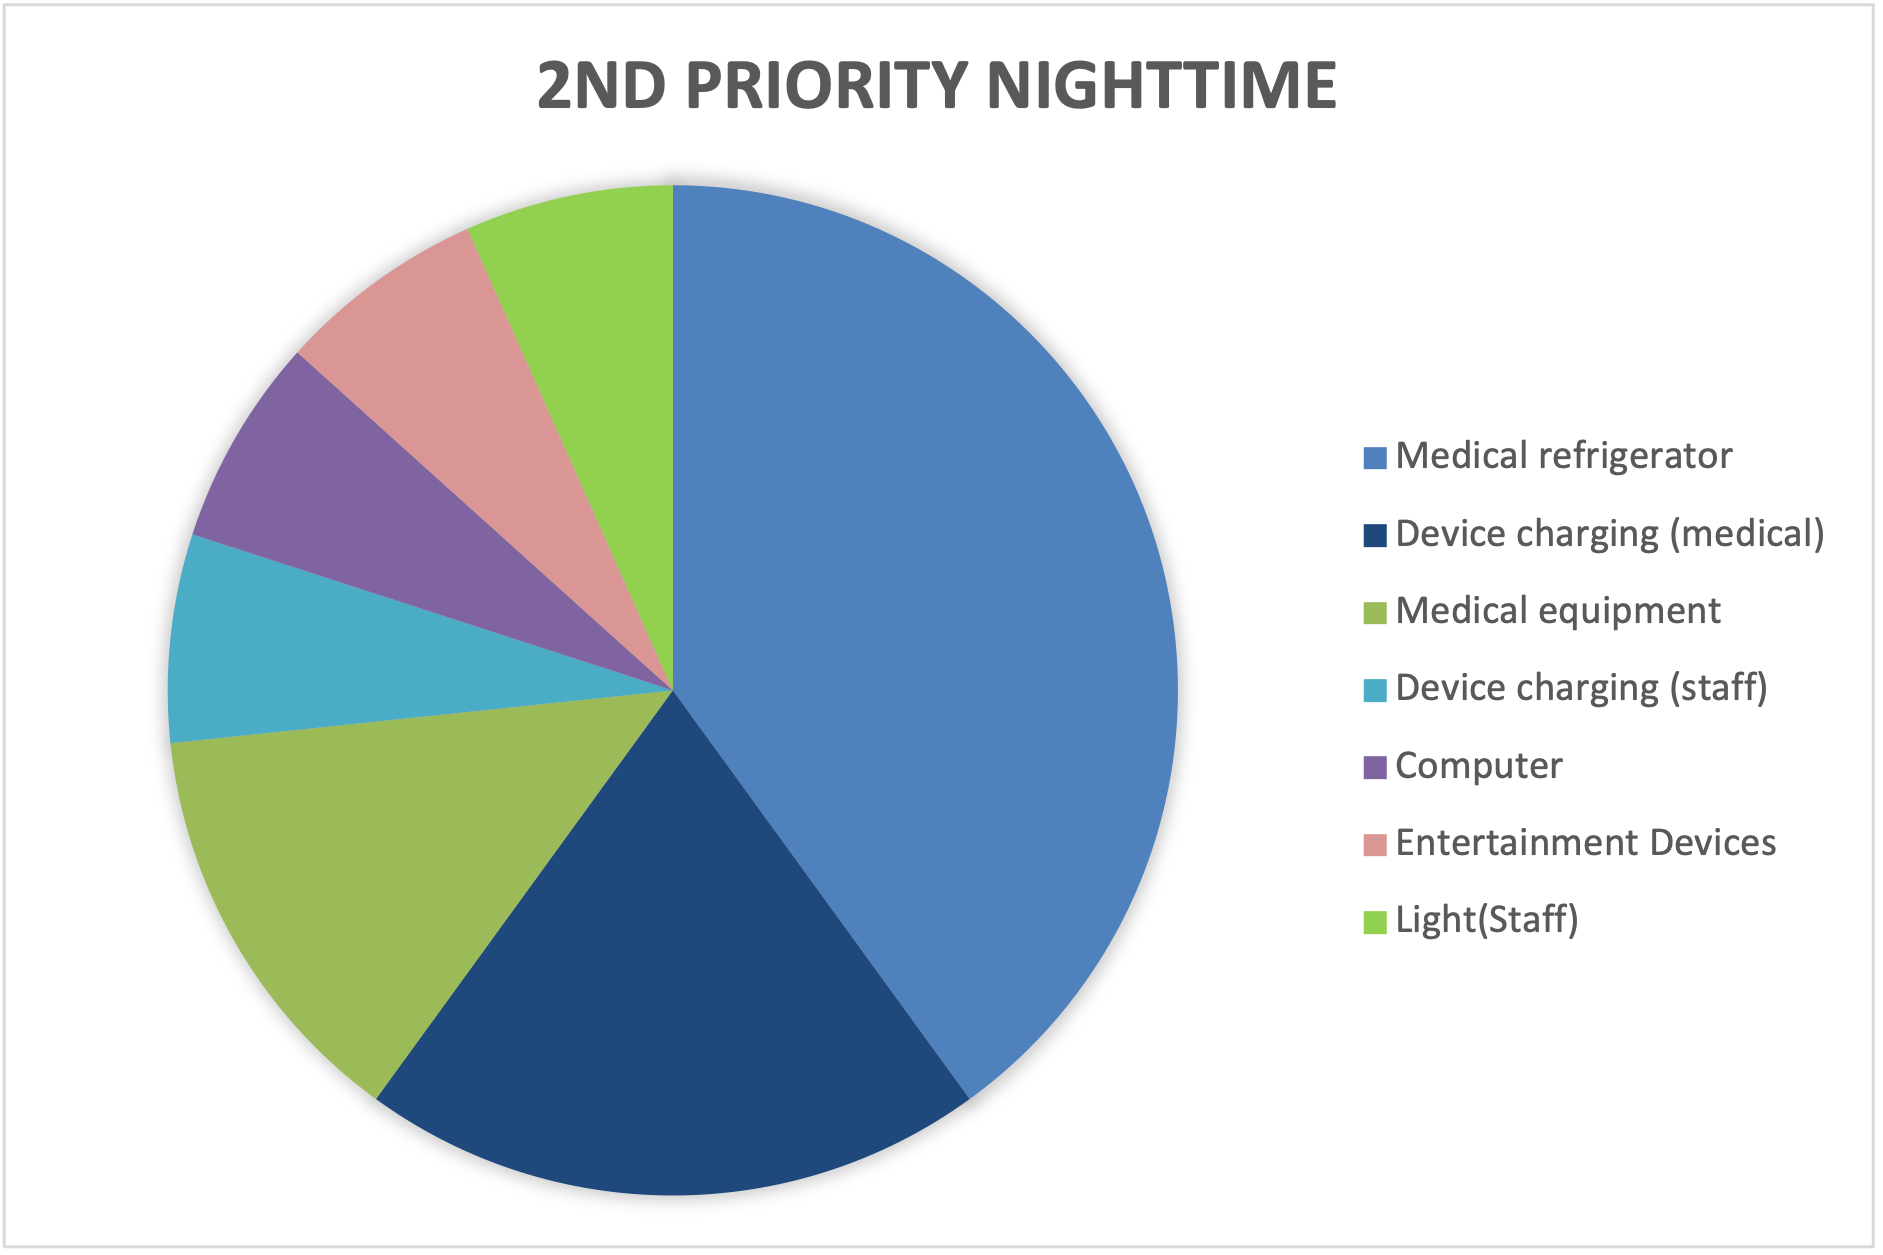
\includegraphics[width=\linewidth]{Figures/06Design/user_survey_load_nighttime_2nd_priority.png}
    \caption[User survey: Nighttime 2nd priority]{Reported 2nd priority amongst loads during nighttime.}
    \label{fig:user_survey_load_nighttime_2nd_priority}
  \end{subfigure}

  \caption[User survey: Nighttime priority]{Reported 1st and 2nd priority amongst loads during nighttime.}
  \label{fig:user_survey_load_nighttime_1st&2nd_priority}
\end{figure}



\subsection{Load classification}\label{seq:load_classification}
As seen in the previous section, there are several different kinds of loads installed at the various sites. These vary in their importance for the operation at the site, their electrical characteristics and the characteristics important for controlling the system. Using the classification from \cite{Philipo2022-rx}, the classifying control characteristics are \todo{check break}
\begin{itemize}
    \item \textit{Deferable} -   The ability to defer a load to a different time without a penalty. This is only possible if a demand does not need to be instantaneously met. For instance, if the demand for light, TV or Microscope is not met immediately when demanded, it is noticed by the user. Other loads, such as the water pump, does not have this requirement. Although the demand for water is non-deferable, the pump itself supplies water to a tank, hence as long as the tank has water there is no penalty for deferring the running of the water pump. 
    \item \textit{Dimable}  -   A dimable load can run on various power levels
    \item \textit{Interuptable} -   A interuptable load can be interrupted after being started without any additional penalty. 
\end{itemize}

In addition to these, loads are also assigned a priority, which translates into a penalty for not being allowed to run when demanded. As seen from the user survey, the end-users value different loads higher at different times. The priority is therefore not static, but may change during the day. The various loads found to be connected during the user survey is classified in table \ref{tab:load_control} \\

\begin{table}[]
    \centering
    \small
    \begin{tabular}{|>{\raggedright\arraybackslash}p{4cm}|p{1.5cm}|p{1.5cm}|p{2cm}|}
         Load & Deferable & Dimable & Interuptable \\
         \hline
         Lights (Medical/School) & NO & NO & NO\\
         Phone/Laptop Charging (Medical) & YES & YES & YES\\
         Oxygen Concentrator & NO & NO & NO\\
         HIV diagnosis equipment & NO & NO & NO\\
         Sterilizer & NO & NO & YES\\
         Microscope & NO & NO & NO\\
         Refrigerator (Medical) & NO & NO & NO\\
         \hline
         Light (Staff) & NO & NO & NO\\
         Phone/Laptop Charging (Staff) & YES & YES & YES\\
         Entertainment & NO & NO & NO\\
         Refrigerator (Staff) & NO & NO & NO\\                  
         Cooking appliances & NO & NO & NO\\
         \hline
         Water pump & YES & YES & YES\\
         Water heater & YES & YES & YES\\
         \hline
    \end{tabular}
    \caption[Connected loads control attributes]{Loads connected to the systems with their control attributes}
    \label{tab:load_control}
\end{table}

As mentioned in section \ref{seq:data_collection}, loads are not measured individually, but based on the circuit they are connected to. While there could potentially be a method of identifying a specific load through the consumption measured from the circuit, this has not been attempted in this thesis. As a result, the resolution of classification decreases to the circuit level. Mapping the control characteristics from \autoref{tab:load_control} to the circuits in \autoref{tab:loads_chiwoza} yields the circuit level control characteristics in \autoref{tab:circuit_control}. For the rest of the design, this will be the level of resolution, the term load is therefore broadened to include all individual loads connected to a circuit. 

\begin{table}[]
    \centering
    \small
    \begin{tabular}{|>{\raggedright\arraybackslash}p{4cm}|p{1.5cm}|p{1.5cm}|p{2cm}|}
         Circuit & Deferable & Dimable & Interuptable \\
         \hline
         Medical Light & NO & NO & NO\\
         Medical Socket & NO & NO & NO\\
         Staff Light 1-3 & NO & NO & NO\\
         Staff Socket 3 & NO & NO & NO\\
         Guardian Shelter Light & NO & NO & NO\\
         Guardian Shelter Socket & NO & NO & NO\\
         Fence Light & NO & NO & NO\\
         \hline
         Water pump & YES & YES & YES\\
         Water heater & YES & YES & YES\\
         \hline
         Solar Maize Mill & YES & YES & YES\\
         Rental Batteries & YES & YES & YES\\
         \hline
    \end{tabular}
    \caption[Circuits control attributes]{Circuits connected to the systems with their control attributes}
    \label{tab:circuit_control}
\end{table}

\subsubsection{Flexible Loads definition and analysis}\label{seq:flex_loads}
From a control perspective, the last 4 loads of table \ref{tab:circuit_control} are the most interesting. Because their demand is flexible, they offer the prime control option to be utilized. These \textit{flexible loads} are characterized by the following:
\begin{itemize}
    \item \textit{Energy Demand}    -   Within a day, these loads demands to be ran enough to perform some task. For the water pump, this will be to fill the tank with enough water to satisfy a days consumption, if the tank is large enough to support that. For the water heater, this will be to heat enough water to last X hours in the future. The key is that the energy demand does not have to be satisfied immediately, but within some time window.
    \item \textit{Power Demand}     -   If the flexible load is running, it is required a certain amount of power to be able to run. This is the power demand. 
    \item \textit{Operation Window} -   The operation window specifies within which time window a flexible load can run. For instance, the solar Maize mill should be running during the day, because that is when the farmers can deliver and collect their goods.   
\end{itemize}

As these loads are more clearly defined, the values can be found from datasheets\cite{wp_documentation}\cite{water_heater}\cite{maize_mill}. The water pump at Chiwoza is a \textit{SQF5-70} from Grundfos. These are powered by  a \textit{universal motor}. A universal motor can be controlled by regulating the current supplied to the motor. Figure \ref{fig:wp_power_flow_curve} from the datasheet provided by the manufacturer relates the power to water depth and flow. Similarly, the figures for the power rating for the other flexible loads are found in the datasheets and included in \ref{tab:flexible_loads_characteristics}. The daily energy demand for the water pump and heater is determined as the average historical daily demand. For the two loads that have not been connected, the maize mill and rental batteries, their daily demand is determined through internal economic calculations by DCP on how often they need to run to be economically feasible for DCP to install at the sites.\\

\begin{figure}
    \centering
    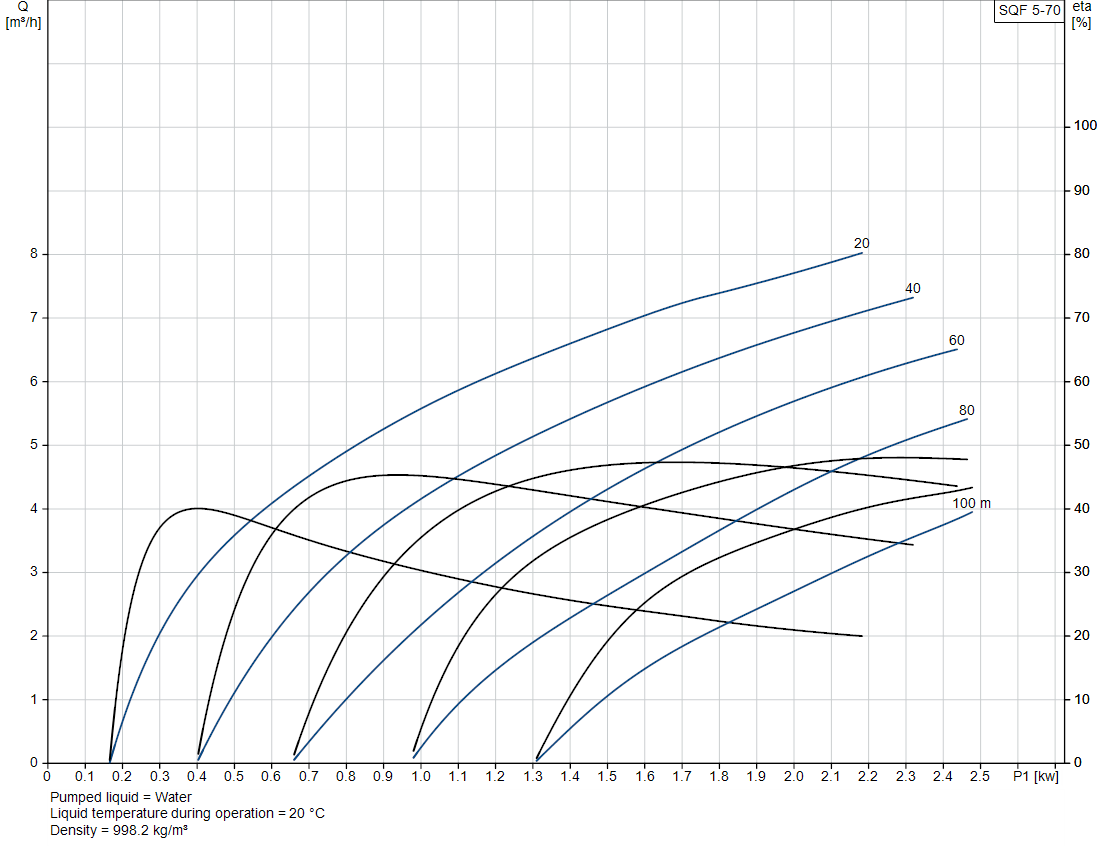
\includegraphics[width=\textwidth]{Figures/06Design/wp_sqf25-2_power_curve.png}
    \caption[Water pump power/flow-curve]{Power-flow curve for the water pump installed at Chiwoza. Along the y-axis is the flow measured in [m2/h] while along the x-axis is the power in kW. The blue lines show the depth of the well.}
    \label{fig:wp_power_flow_curve}
\end{figure}

\begin{table}[]
    \centering
    \begin{tabular}{c|c|c|c|c}
       Load  & Min Power (W) & Max Power (W)& Energy Demand Daily (Wh) \\
       \hline
       Water Pump  & 400 & 1100 & 2750 \\
       Water Heater  & 200 & 350 & 1400 \\
       Rental Batteries  & 10.8 & 270 & 540 \\
       Maize Mill  & 800 & 3000 & 9750 \\
    \end{tabular}
    \caption[Flexible Loads energy characteristics]{Flexible Loads energy characteristics}
    \label{tab:flexible_loads_characteristics}
\end{table}

It is evident that most loads can neither be deferred, dimmed or interrupted without a penalty. These loads are inflexible, their demand can not be shifted or reduced, it either has to be met or not met. For these loads, it becomes important to predict the demand, so that one can adjust accordingly. The forecasting of inflexible loads are the key idea of the following chapter. 


\section{Load Forecasting }\label{seq:load_forecasting}

Instantaneous consumption is measured by the system. Knowing how demand will behave in the future enables informed decision-making on how to allocate produced energy between loads and the battery for the optimal operation within a determined time-window. As demand is neither known fully in advance nor fully deterministic on past and current conditions, the process of making predictions about future demand is non-trivial. For this application, several \textit{persistence} and \textit{ARIMA} models were developed and implemented to better the accuracy of forecasted future demand.\\

The process for load forecasting in this thesis consists of the following steps:
\begin{itemize}
    \item \textbf{Develop Persistence model}
    \begin{itemize}
        \item Find suitable look-back period candidates by forecasting over a small time frame
        \item Find the best candidate by testing candidates over a larger time frame 
    \end{itemize}
    \item \textbf{Develop ARIMA model}
    \begin{itemize}
        \item Identify inter-day periodicity, meaning patterns between days. Use this to find suitable periodic coefficients.
        \item Identify intra-day periodicity, meaning patterns within a day. Differentiate until stationary within a day.
        \item For each level of differentiation, find suitable candidates by looking at the ACF and PACF.
    \end{itemize} 
    \item \textbf{Compare ARIMA candidates against each other and the best persistence model by testing over a longer time-frame}
\end{itemize}

The process has to be performed for every circuit connected to the system. However, within this section, the process in its entirety will only be illustrated for one specific meter - \textit{The medical light at Chiwoza}. The other meters will be included at the end of this section with their starting point and resulting best model found from the analysis.\\

\subsection{Persistence Model}
As outlined in section \ref{seq:stat_forecasting}, a persistence model is amongst the simplest and most intuitive models for forecasting. It serves as a baseline against which to compare the more advanced models.\\

Based on the analysis in \ref{seq:periodicity}, past consumption is expected to contain information about future consumption. Hence a \textit{unweighted average persistence} model was developed to forecast the consumption of each meter. The model is a compromise between the accuracy and complexity of tuning.\\

The models were tested by a range of look-back periods estimating the consumption of all hours of a single day. The \textit{MAE} between the forecasted and actual consumption was used to compare the models. This yielded a daily plot like \ref{fig:maeVlookback_chiwoza_med_light_20231128}. From this, a few candidates could be picked for testing over a longer period. This was done in figure \ref{fig:maeVlookback_chiwoza_med_light202311}. The difference between the plots can be difficult to assert from the plot. Considering the average MAE across the whole month, shown in \ref{tab:avg_mae_chiwoza_med_persistence_2023}, a model with a look-back period of 32 days yields the lowest value. An average MAE of 0.052 means that an error of 52W is expected. In the plot in figure \ref{fig:maeVlookback_chiwoza_med_light202311} a look-back period of 3 days yields the lowest maximum MAE of about 90W. The choice of model depends on the intended usage. Because the persistence model will in this design be used as a baseline to compare the ARIMA, the model with the best average MAE will be chosen.  

\begin{figure}
    \centering
    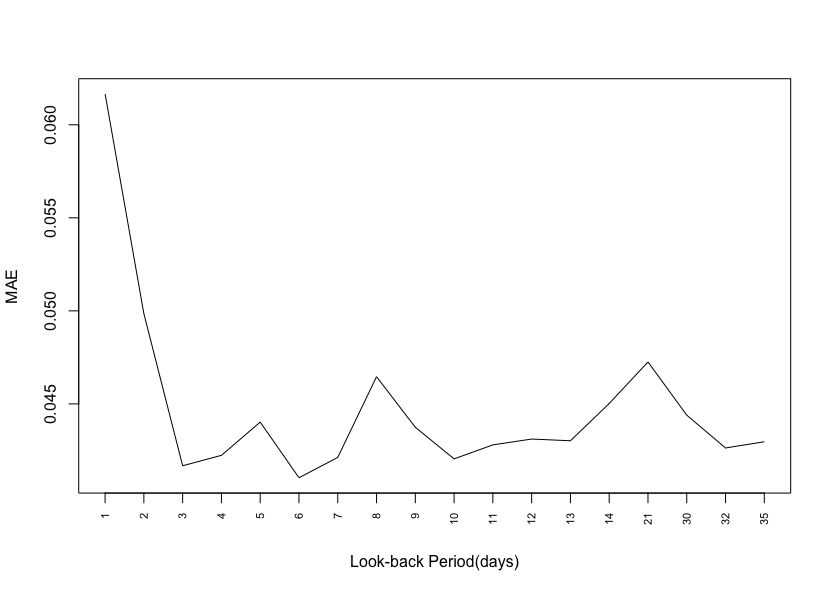
\includegraphics[width=\textwidth]{Figures/06Design/maeVlookback_chiwoza_med_light_20231128.png}
    \caption[MAE vs lookback-period Medical Light Chiwoza 20231128]{MAE vs Look-back period for medical light consumption at Chiwoza 2023-11-28.}
    \label{fig:maeVlookback_chiwoza_med_light_20231128}
\end{figure}

\begin{figure}
    \centering
    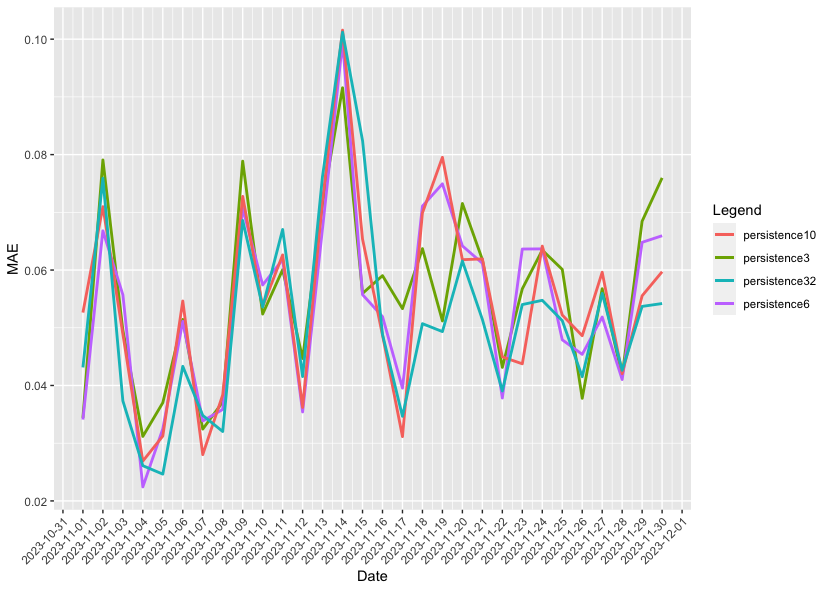
\includegraphics[width=\textwidth]{Figures/06Design/maeVlookback_chiwoza_med_light_202311.png}
    \caption[MAE vs look-back Medical light 202311]{MAE vs Look-back period for medical light consumption at Chiwoza during the whole of November 2023. Using four persistence models with different look-back period \textit{k}. (green:\textit{k}=3, purple:\textit{k}=6, red:\textit{k}=10), turquoise:\textit{k}=32)}
    \label{fig:maeVlookback_chiwoza_med_light202311}
\end{figure}

\begin{table}[]
    \centering
    \begin{tabular}{c|c}
         Look-back period (days)& Average MAE  \\
         3& 0.056\\
         6& 0.054\\
         10& 0.055\\
         32& 0.052
    \end{tabular}
    \caption[Average MAE persistence models]{Caption}
    \label{tab:avg_mae_chiwoza_med_persistence_2023}
\end{table}

\subsection{ARIMA Model}
The second model used for load forecasting is the ARIMA-model. The model was selected because it is purely statistical without the need for a priori data. As mentioned in \ref{seq:stat_forecasting}, an ARIMA model is a statistical forecasting model combining an auto-regressive and moving average model with a differentiating term. Through the analysis both intra- and inter-day periodicity was discovered for several of the meters, hence a SARIMA model is appropriate. To design a SARIMA model for each meter to be forecasted, the following terms must be determined
\begin{itemize}
    \item \textit{p}    -   The order of the auto-regressive model.
    \item \textit{d}    -   The differentiating order.
    \item \textit{q}    -   The order of the moving average model.
    \item \textit{P}    -   The order of the auto-regressive model shifted back one period.
    \item \textit{D}    -   The amount of terms one period back shifted to include directly.
    \item \textit{Q}    -   The order of the moving average model shifted back one period.
    \item \textit{s}    -   The period of the time series.
\end{itemize}

Of these, only the time series period, \textit{s}, is known in advance. From the analysis, it is known that the consumption follows a daily cycle. The period is therefore equal to the number of samples within a day, which if done on an hourly basis equals 24.\\

The other parameters is to be obtained through a statistical analysis of the time-series for each meter. The first step of this process is to examine the original time-series for a given meter. Figure \ref{fig:con_ts_chiwoza_med_light_20231110-25} showcasing the consumption from medical lights at Chiwoza is a seemingly stationary time-series. The series oscillates, but there is no evident trend. This suggests stationarity. Further evidence can be found be using the augmented dicker-fuller test, where the results are shown in \ref{tab:result_dicker-fuller} strongly reject the null hypothesis of non-stationarity between the days. Figure \ref{fig:con_acf_h_chiwoza_med_light_20231110-25} confirms this, as the ACF decreases to zero after a few lags. This means that the auto-regressive and moving average model can be utilized without differentiating the time-series first. Although it is still possible that one can achieve better results by a differentiated time-series.\\


\begin{figure}
    \centering
    \includegraphics[width=\linewidth]{Figures/06Design/con_ts_chiwoza_med_light_20231110-25.png}
    \caption[Medical Light consumption Chiwoza 20231110-1125]{Consumption medical light Chiwoza as a time-series between 2023-11-10 and 2023-11-25.}
    \label{fig:con_ts_chiwoza_med_light_20231110-25}
\end{figure}

\begin{figure}
    \centering
    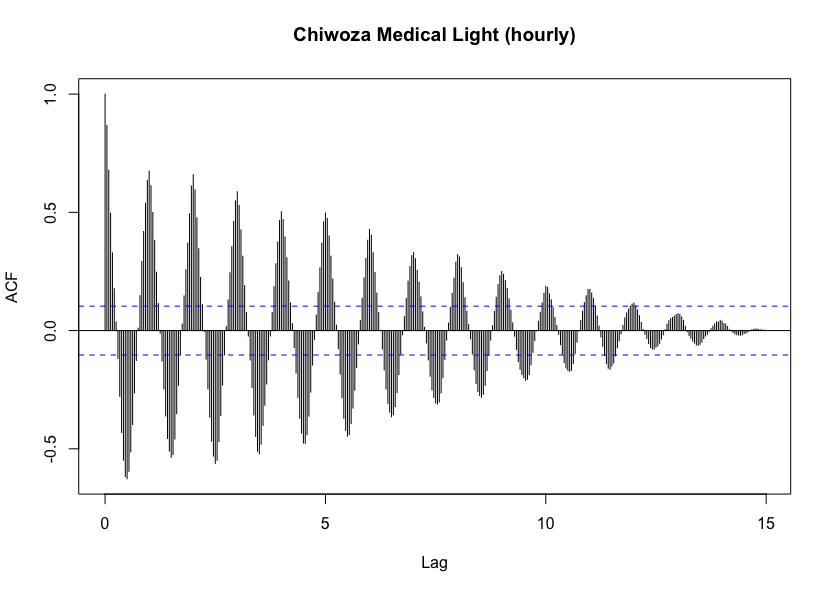
\includegraphics[width=\textwidth]{Figures/06Design/con_acf_h_chiwoza_med_light_20231110-25.png}
    \caption[ACF Medical Light consumption Chiwoza 20231110-1125]{ACF of the hourly consumption of the medical lights at Chiwoza between 2023-11-10 and 2023-11-25.}
    \label{fig:con_acf_h_chiwoza_med_light_20231110-25}
\end{figure}


\begin{table}[]
    \centering
    \begin{tabular}{c|c|c|c}
    Meter & DF & p-value & time range \\
    \hline
    Medical Lights Chiwoza & -9.0046 & <0.01 & 2023-11-10 - 2023-11-25
    \end{tabular}
    \caption[Dicker-Fuller test]{The results of the Augmented-Dicker-Fuller test}
    \label{tab:result_dicker-fuller}
\end{table}

Within a day, we know that there is a seasonal pattern. Looking at figure \ref{fig:con_acf_h_chiwoza_med_light_20231125} this means that the ACF does not decay, and an MA-model cannot be utilized. The PACF however, shown in \ref{fig:con_pacf_h_chiwoza_med_light_20231125} shows clear contributions from certain terms. A pure auto-regressive model combined with some seasonal terms is therefore a candidate. Differentiating the time-series and finding the ACF and PACF within a day produces the plots shown in \ref{fig:con_d_acf_pacf_h_chiwoza_med_light_20231125}. Here the ACF plot decays faster, meaning that a candidate with a differential term can be included.\\

\begin{figure}
  \centering

  % First Subfigure
  \begin{subfigure}{\textwidth}
    \centering
    \includegraphics[width=\linewidth]{Figures/06Design/con_acf_h_chiwoza_med_light_20231125.png}
    \caption[ACF Medical light consumption 20231110]{ACF of hourly medical light consumption Chiwoza at 2023-11-10.}
    \label{fig:con_acf_h_chiwoza_med_light_20231125}
  \end{subfigure}

  % Add some vertical space between the subfigures
  \vspace{0.5cm}

  % Second Subfigure
  \begin{subfigure}{\textwidth}
    \centering
    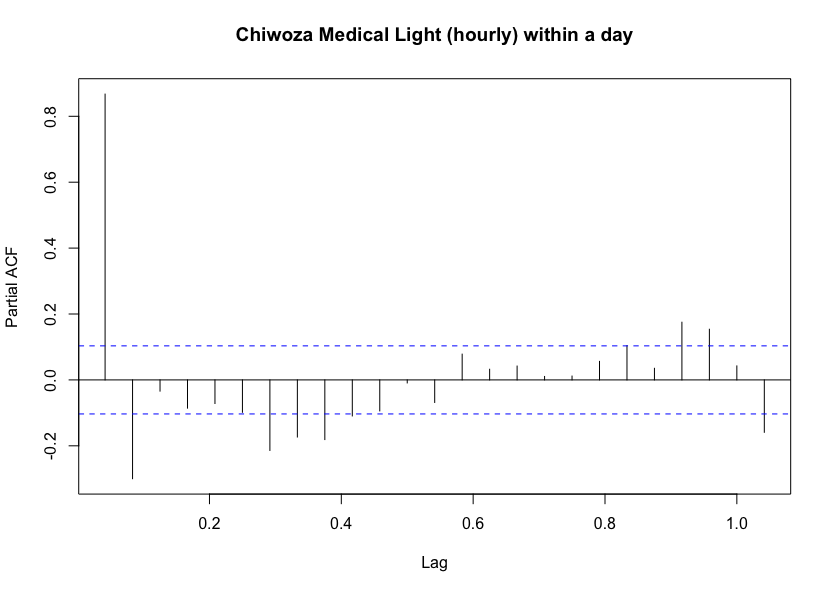
\includegraphics[width=\linewidth]{Figures/06Design/con_pacf_h_chiwoza_med_light_20231125.png}
    \caption[ACF Medical light consumption 20231110]{PACF of hourly medical light consumption Chiwoza at 2023-11-10.}
    \label{fig:con_pacf_h_chiwoza_med_light_20231125}
  \end{subfigure}

  \caption[ACF and PACF Medical light consumption 20231110]{ACF and PACF of hourly medical light consumption Chiwoza at 2023-11-10.}
  \label{fig:con_acf_pacf_h_chiwoza_med_light_20231125}
\end{figure}

\begin{figure}
  \centering

  % First Subfigure
  \begin{subfigure}{\textwidth}
    \centering
    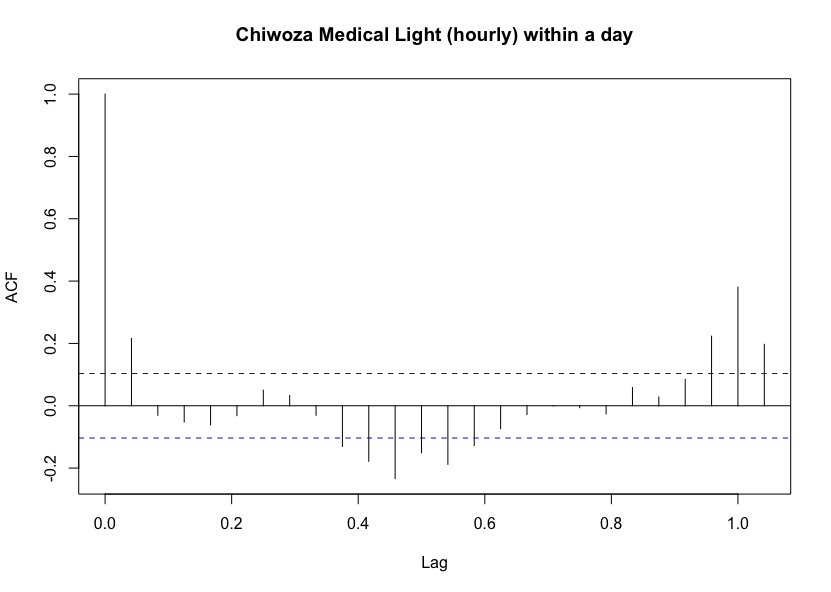
\includegraphics[width=\linewidth]{Figures/06Design/con_d_acf_h_chiwoza_med_light_20231125.png}
    \caption[ACF differentiated Medical light consumption 20231110]{ACF of differentiated hourly medical light consumption Chiwoza at 2023-11-10.}
    \label{fig:con_d_acf_h_chiwoza_med_light_20231125}
  \end{subfigure}

  % Add some vertical space between the subfigures
  \vspace{0.5cm}

  % Second Subfigure
  \begin{subfigure}{\textwidth}
    \centering
    \includegraphics[width=\linewidth]{Figures/06Design/con_d_pacf_h_chiwoza_med_light_20231125.png}
    \caption[PACF differentiated medical light consumption 20231110]{PACF of differentiated  hourly medical light consumption Chiwoza at 2023-11-10.}
    \label{fig:con_d_pacf_h_chiwoza_med_light_20231125}
  \end{subfigure}

  \caption[ACF and PACF differentiated medical light consumption 20231110]{ACF and PACF of differentiated hourly medical light consumption Chiwoza at 2023-11-10.}
  \label{fig:con_d_acf_pacf_h_chiwoza_med_light_20231125}
\end{figure}

Section \ref{seq:tuning_arima} outlines the process of finding the \textit{p} and \textit{q} values of the model using the partial auto-correlation function (PACF) and the auto-correlation function(ACF) respectively. From figure \ref{fig:con_d_acf_pacf_h_chiwoza_med_light_20231125} we see that ARIMA(1,1,2)(1,1,1) can be a candidate. There is however still seasonality apparent in figure \ref{fig:con_d_acf_h_chiwoza_med_light_20231125}. Differentiating the time-series again removes all intra-day seasonality, as seen in figure \ref{fig:con_d2_acf_h_chiwoza_med_light_20231125} by the complete decay of the ACF besides the full lag. Combined with the PACF plot in figure \ref{fig:con_d2_pacf_h_chiwoza_med_light_20231125} we see that ARIMA(1,2,2)(1,1,1) could be another candidate. \\

\begin{figure}
  \centering

  % First Subfigure
  \begin{subfigure}{\textwidth}
    \centering
    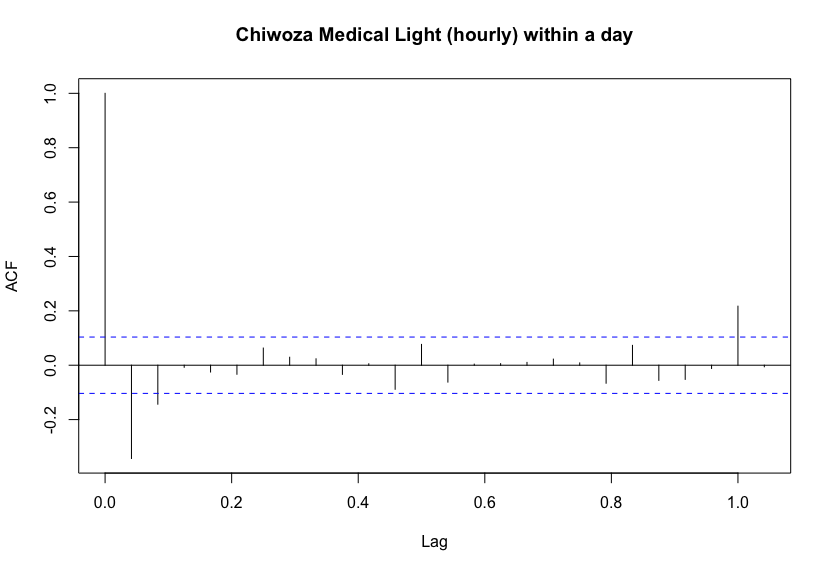
\includegraphics[width=\linewidth]{Figures/06Design/con_d2_acf_h_chiwoza_med_light_20231125.png}
    \caption[ACF second order differentiated medical consumption 20231110]{ACF of second order differentiated hourly medical light consumption Chiwoza at 2023-11-10.}
    \label{fig:con_d2_acf_h_chiwoza_med_light_20231125}
  \end{subfigure}

  % Add some vertical space between the subfigures
  \vspace{0.5cm}

  % Second Subfigure
  \begin{subfigure}{\textwidth}
    \centering
    \includegraphics[width=\linewidth]{Figures/06Design/con_d2_pacf_h_chiwoza_med_light_20231125.png}
    \caption[PACF second order differentiated medical consumption 20231110]{PACF of second order differentiated  hourly medical light consumption Chiwoza at 2023-11-10.}
    \label{fig:con_d2_pacf_h_chiwoza_med_light_20231125}
  \end{subfigure}

  \caption[ACF and PACF second order differentiated medical consumption 20231110]{ACF and PACF of second order differentiated hourly medical light consumption Chiwoza at 2023-11-10.}
  \label{fig:con_d2_acf_pacf_h_chiwoza_med_light_20231125}
\end{figure}

The three candidate listed in \ref{tab:arima_candidate_chiwoza_med_light} can be implemented and tested over a wider time period. Model III looks clearly worse from the plot, but it is difficult separating I and II. From table \ref{tab:arima_candidate_mae_chiwoza_med_light} we see that model II performed slightly better on average MAE over the month of November. It also has a lower maximum MAE than model I. Of the ARIMA models, only I and II managed to beat the baseline set by the persistence model. Looking at the forecasted time-series for November from model II versus the actual time-series in figure \ref{fig:atVSft_chiwoza_medical_light_202311} , the model has acceptable performance. 

\begin{table}[]
    \centering
    \begin{tabular}{c|c}
         \#& model \\
         \hline
         I& ARIMA(2,0,0)(1,1,1)\\
         II& ARIMA(1,1,2)(1,1,1)\\
         III& ARIMA(1,2,2)(1,1,1)\\
    \end{tabular}
    \caption[ARIMA candidates medical light consumption Chiwoza]{ARIMA model candidates for medical light consumption Chiwoza}
    \label{tab:arima_candidate_chiwoza_med_light}
\end{table}

\begin{figure}
    \centering
    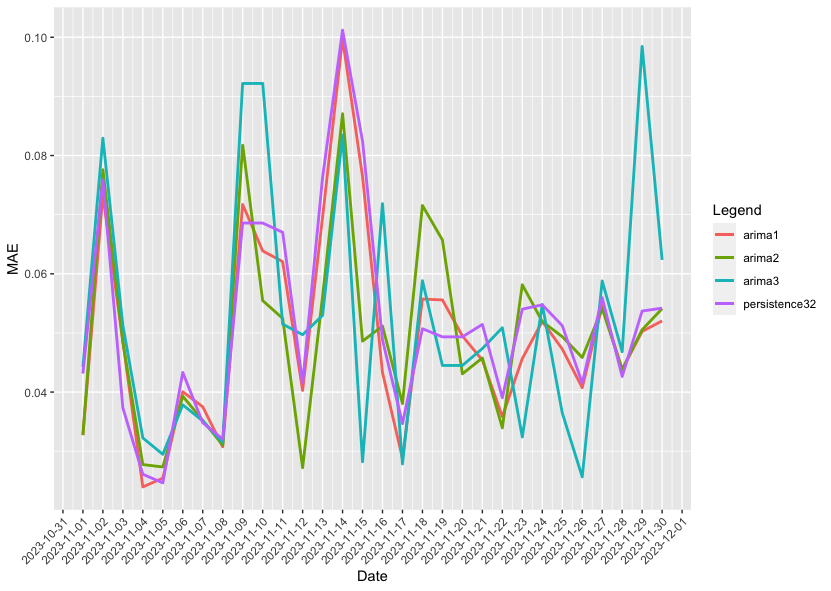
\includegraphics[width=\textwidth]{Figures/06Design/mae_arima_chiwoza_med_light_202311.png}
    \caption[MAE ARIMA candidates medical light consumption Chiwoza]{MAE of the 3 ARIMA models listed in \ref{tab:arima_candidate_chiwoza_med_light} over the month of November 2023.Included is also the MAE of a persistence model with look-back period of 32 days}
    \label{fig:mae_arima_chiwoza_med_light_202311}
\end{figure}

\begin{table}[]
    \centering
    \begin{tabular}{c|c}
         \#& average MAE \\
         \hline
         I& 0.049\\
         II& 0.049\\
         III& 0.052\\
         $persistence_{32}$& 0.052\\
    \end{tabular}
    \caption[Average MAE ARIMA candidates and persistence model medical light consumption Chiwoza]{ARIMA model candidates' MAE for medical light consumption estimation over the month of November at Chiwoza. Included is the average MAE of a persistence model with look-back period of 32 days.}
    \label{tab:arima_candidate_mae_chiwoza_med_light}
\end{table}

\begin{figure}
    \centering
    \includegraphics[width=\textwidth]{Figures/06Design/atVSft_chiwoza_medical_light_202311.png}
    \caption[Actual vs Forecasted consumption medical light consumption]{The actual hourly consumption vs the forecast from the ARIMA model II in \ref{tab:arima_candidate_chiwoza_med_light} for medical light consumption Chiwoza November 2023.}
    \label{fig:atVSft_chiwoza_medical_light_202311}
\end{figure}

As mentioned earlier in this section, this process of selecting ARIMA candidates, comparing them against each other and a persistence model has to be repeated for all the loads connected to a system that is to be forecasted. The result of this is shown in \ref{tab:load_forecasting_results_chiwoza}. In section \ref{seq:periodicity}, some loads, like the Guardian shelter Socket was found to have a strong weekday pattern. To accommodate for this, the ARIMA was modified to include this behavior. The algorithm, shown in \ref{alg:arima_forecast_periodic}, runs a different ARIMA model for weekdays and weekend. Furthermore, when gathering historic data for its forecast, it discards days it has been asked to ignore. In \ref{fig:forecasting_results_chiwoza_guard_socket} this is seen as a model which is able to handle the shape of high consumption during the week and none during weekend.

\begin{algorithm}
\caption{ARIMA forecaster weekday periodic}\label{alg:arima_forecast_periodic}
\begin{algorithmic}
    \State$dow = dayOfWeek(date) $
    \If{$dow == Sat | dow == Sun$}
        \State$ignoreDays = (Mon,Tue,Wed,Thu,Fri)$
        \State$model \gets arimaWeekendParam$
    \Else
        \State$ignoreDays = (Sat,Sun)$
        \State$model \gets arimaWeekdayParam$
    \EndIf
    \State$historicData \gets getHistoricData(ignoreDays)$
    \State$forecast \gets arimaForecast(model, historicData)$
\end{algorithmic}
\end{algorithm}

\begin{figure}
% First Subfigure
    \begin{subfigure}{\textwidth}
    \centering
    \includegraphics[width=\linewidth]{Figures/06Design/con_ts_chiwoza_staff_light1_20231101-26.png}
    \caption{Light consumption at staff house 1 Chiwoza during November.}
    \label{fig:con_ts_chiwoza_staff_light1_20231101-26}
  \end{subfigure}

  % Add some vertical space between the subfigures
  \vspace{0.5cm}

  % Second Subfigure
  \begin{subfigure}{\textwidth}
    \centering
    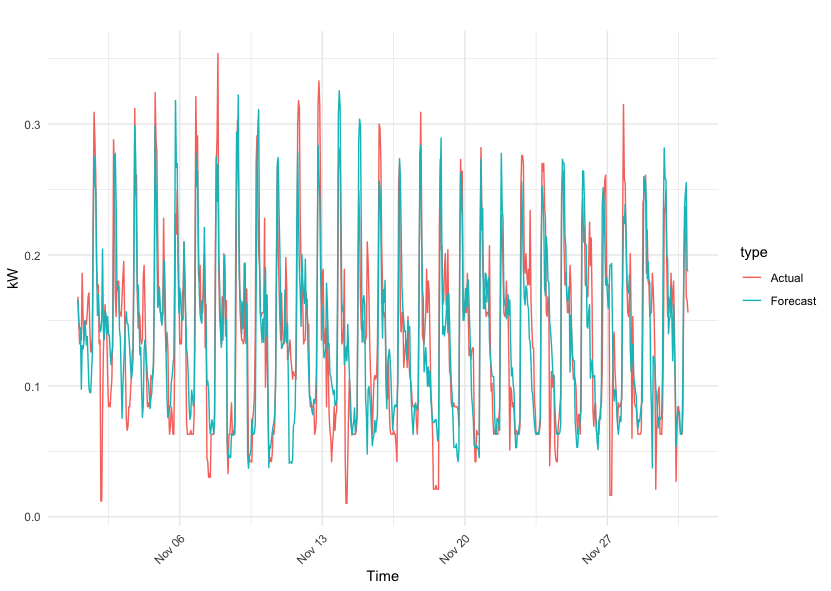
\includegraphics[width=\linewidth]{Figures/06Design/atVSft_chiwoza_staff_light1_202311.png}
    \caption{The actual vs the forecasted hourly light consumption for Chiwoza Staff house 1.}
    \label{fig:atVSft_chiwoza_staff_light1_202311}
  \end{subfigure}

  \caption[Light consumption staff house 1 forecasting]{Starting point and result load forecasting for light consumption for Chiwoza Staff house 1.}
  \label{fig:forecasting_results_chiwoza_staff_light1}
\end{figure}

\begin{figure}
% First Subfigure
    \begin{subfigure}{\textwidth}
    \centering
    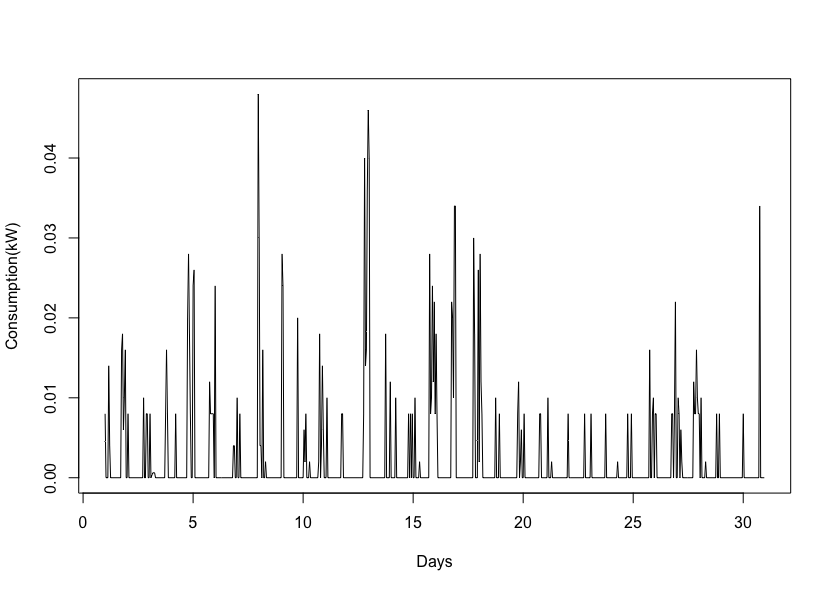
\includegraphics[width=\linewidth]{Figures/06Design/con_ts_chiwoza_staff_light2_20231101-30.png}
    \caption{Light consumption at staff house 2 Chiwoza during November.}
    \label{fig:con_ts_chiwoza_staff_light2_202311}
  \end{subfigure}

  % Add some vertical space between the subfigures
  \vspace{0.5cm}

  % Second Subfigure
  \begin{subfigure}{\textwidth}
    \centering
    \includegraphics[width=\linewidth]{Figures/06Design/atVSft_chiwoza_staff_light2_202311.png}
    \caption{The actual vs the forecasted hourly light consumption for Chiwoza Staff house 2.}
    \label{fig:atVSft_chiwoza_staff_light2_202311}
  \end{subfigure}

  \caption[Light consumption staff house 2 forecasting]{Starting point and result load forecasting for light consumption for Chiwoza Staff house 2.}
  \label{fig:forecasting_results_chiwoza_staff_light2}
\end{figure}

\begin{figure}
% First Subfigure
    \begin{subfigure}{\textwidth}
    \centering
    \includegraphics[width=\linewidth]{Figures/06Design/con_ts_chiwoza_staff_light3_202311.png}
    \caption{Light consumption at staff house 3 Chiwoza during November.}
    \label{fig:con_ts_chiwoza_staff_light3_20231001-20}
  \end{subfigure}
  
  % Add some vertical space between the subfigures
  \vspace{0.5cm}

  % Second Subfigure
  
  \begin{subfigure}{\textwidth}
    \centering
    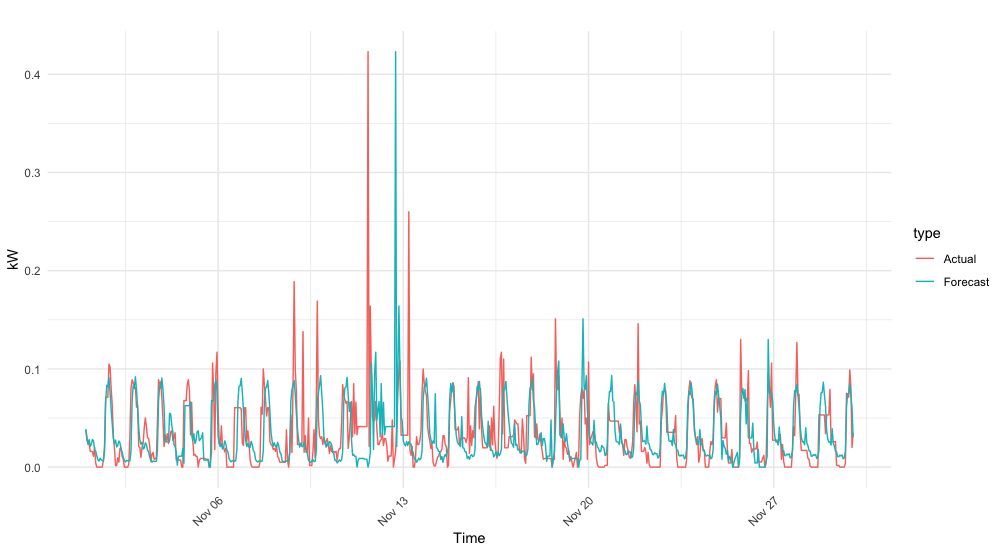
\includegraphics[width=\linewidth]{Figures/06Design/atVSft_chiwoza_staff_light3_202311.png}
    \caption{The actual vs the forecasted hourly light consumption for Chiwoza Staff house 3.}
    \label{fig:atVSft_chiwoza_staff_light3_20231001-20}
  \end{subfigure}


  \caption[Light consumption staff house 3 forecasting]{Starting point and result load forecasting for light consumption for Chiwoza Staff house 3.}
  \label{fig:forecasting_results_chiwoza_staff_light3}
\end{figure}

\begin{figure}
% First Subfigure
    \begin{subfigure}{\textwidth}
    \centering
    \includegraphics[width=\linewidth]{Figures/06Design/con_ts_chiwoza_fence_light_202310.png}
    \caption{Hourly consumption for the Chiwoza Fence light during October 2023.}
    \label{fig:con_ts_chiwoza_fence_light_202310}
  \end{subfigure}

  % Add some vertical space between the subfigures
  \vspace{0.5cm}

  % Second Subfigure
  \begin{subfigure}{\textwidth}
    \centering
    \includegraphics[width=\linewidth]{Figures/06Design/atVSft_chiwoza_fence_light_202310.png}
    \caption{The actual vs the forecasted hourly consumption for the Chiwoza Fence light.}
    \label{fig:atVSft_chiwoza_fence_light_202310}
  \end{subfigure}

  \caption[Fence Light consumption forecasting]{Starting point and result load forecasting for hourly consumption for the Chiwoza Fence light.}
  \label{fig:forecasting_results_chiwoza_fence_light}
\end{figure}

\begin{figure}
% First Subfigure
    \begin{subfigure}{\textwidth}
    \centering
    \includegraphics[width=\linewidth]{Figures/06Design/con_ts_chiwoza_guard_light_202311.png}
    \caption{Hourly consumption for the Chiwoza Guardian Shelter light during November 2023.}
    \label{fig:con_ts_chiwoza_guard_light_202311}
  \end{subfigure}

  % Add some vertical space between the subfigures
  \vspace{0.5cm}

  % Second Subfigure
  \begin{subfigure}{\textwidth}
    \centering
    \includegraphics[width=\linewidth]{Figures/06Design/atVSft_chiwoza_guard_light_202311.png}
    \caption{The actual vs the forecasted hourly consumption for the Chiwoza Guardian Shelter light.}
    \label{fig:atVSft_chiwoza_guard_light_202311}
  \end{subfigure}

  \caption[Guardian Shelter consumption forecasting]{Starting point and result load forecasting for hourly consumption for the Chiwoza Guardian Shelter light.}
  \label{fig:forecasting_results_chiwoza_guard_light}
\end{figure}

\begin{figure}
% First Subfigure
    \begin{subfigure}{\textwidth}
    \centering
    \includegraphics[width=\linewidth]{Figures/06Design/con_ts_chiwoza_med_socket_202311.png}
    \caption{Hourly consumption for the Chiwoza medical socket during November 2023.}
    \label{fig:con_ts_chiwoza_med_socket_202311}
  \end{subfigure}

  % Add some vertical space between the subfigures
  \vspace{0.5cm}

  % Second Subfigure
  \begin{subfigure}{\textwidth}
    \centering
    \includegraphics[width=\linewidth]{Figures/06Design/atVSft_chiwoza_med_socket_202311.png}
    \caption{The actual vs the forecasted hourly consumption for the Chiwoza medical socket.}
    \label{fig:atVSft_chiwoza_med_socket_202311}
  \end{subfigure}

  \caption[Medical light socket forecasting]{Starting point and result load forecasting for hourly consumption for the Chiwoza Medical socket.}
  \label{fig:forecasting_results_chiwoza_medical_socket}
\end{figure}

\begin{figure}
% First Subfigure
    \begin{minipage}{0.9\textwidth} % Adjust the width as needed
    \begin{subfigure}{\textwidth}
        \centering
        \includegraphics[width=\linewidth]{Figures/06Design/con_ts_chiwoza_staff_socket3_202311.png}
        \caption{Hourly consumption for the Chiwoza staff socket 3 during November 2023.}
        \label{fig:con_ts_chiwoza_staff_socket3_202311}
    \end{subfigure}
    \end{minipage}

  % Add some vertical space between the subfigures
  \vspace{0.5cm}

  % Second Subfigure
    \begin{minipage}{0.9\textwidth} % Adjust the width as needed
    \begin{subfigure}{\textwidth}
        \centering
        \includegraphics[width=\linewidth]{Figures/06Design/atVSft_chiwoza_staff_socket3_202311.png}
        \caption{The actual vs the forecasted hourly consumption for the Chiwoza staff socket 3.}
        \label{fig:atVSft_chiwoza_staff_socket3_202311}
    \end{subfigure}
    \end{minipage}


  \caption[Staff socket 3 consumption forecasting]{Starting point and result load forecasting for hourly consumption for the Chiwoza staff socket 3.}
  \label{fig:forecasting_results_chiwoza_staff_socket3}
\end{figure}

\begin{figure}
% First Subfigure
    \begin{subfigure}{\textwidth}
    \centering
    \includegraphics[width=\linewidth]{Figures/06Design/con_ts_chiwoza_guard_socket_20231119-1216.png}
    \caption{Hourly consumption for the Chiwoza guardian shelter socket 3 from November 19th to December 16th 2023.}
    \label{fig:con_ts_chiwoza_guard_socket_20231119-1216}
  \end{subfigure}

  % Add some vertical space between the subfigures
  \vspace{0.5cm}

  % Second Subfigure
  \begin{subfigure}{\textwidth}
    \centering
    \includegraphics[width=\linewidth]{Figures/06Design/atVSft_chiwoza_guard_socket_20231119-1216.png}
    \caption{The actual vs the forecasted hourly consumption for the Chiwoza guardian shelter socket 3 from November 19th to December 16th 2023.}
    \label{fig:atVSft_chiwoza_guard_socket_20231119-1216}
  \end{subfigure}

  \caption[Guardian shelter socket consumption forecasting]{Starting point and result load forecasting for hourly consumption for the Chiwoza guardian shelter socket 3 from November 19th to December 16th 2023.}
  \label{fig:forecasting_results_chiwoza_guard_socket}
\end{figure}

\begin{table}[]
    \centering
    \begin{tabular}{c|c|c|c|c}
        Load & Forecasting model & Average MAE (W) & Average (W) & Plot  \\
        \hline
        Medical Light   & ARIMA(1,1,2)(1,1,1) & 25  &  113  &   \ref{fig:atVSft_chiwoza_medical_light_202311}\\
        Medical Socket  & ARIMA(2,1,1)(0,1,1) & 10  &   11  &   \ref{fig:forecasting_results_chiwoza_medical_socket}\\
        Staff Light 1   & ARIMA(1,0,0)(1,1,2) & 26  &  46   &   \ref{fig:forecasting_results_chiwoza_staff_light1}\\
        Staff Light 2   & ARIMA(1,0,0)(1,1,1) & 3   &  6    &   \ref{fig:forecasting_results_chiwoza_staff_light2}\\
        Staff Light 3   & ARIMA(1,0,0)(1,1,0) & 18  &  33   &   \ref{fig:forecasting_results_chiwoza_staff_light3}\\
        Staff Socket 3  & ARIMA(2,0,0)(2,1,0) & 28  &  199  &   \ref{fig:forecasting_results_chiwoza_staff_socket3}\\
        Fence Light     & ARIMA(1,0,1)(2,1,0) & 1.7 &  2.4  &   \ref{fig:forecasting_results_chiwoza_fence_light}\\
        Guardian Shelter Light  & ARIMA(6,1,1)(0,1,1) & 3   &   12  &   \ref{fig:forecasting_results_chiwoza_guard_light}\\
        Guardian Shelter Socket  & ARIMA(1,0,1)(0,1,2) & 1.4  &  1.8  &   \ref{fig:forecasting_results_chiwoza_guard_socket}\\
    \end{tabular}
    \caption[Chiwoza consumption forecasting results]{Loads at Chiwoza with their deduced forecast model.}
    \label{tab:load_forecasting_results_chiwoza}
\end{table}



The forecasting yields large errors, especially when forecasting loads with large spikes in the consumption, such as the Chiwoza medical socket seen in figure \ref{fig:forecasting_results_chiwoza_medical_socket}. Here the forecast have the correct shape, but miss the timing. Sudden and high spikes in consumption are expected to be hard to forecast from statistical data alone. 

\subsection{Forecast update}
In the results from the previous section, consumption has been forecasted once every day, and compared to the actual. Instead in the proposed control system, a new forecast will be made every time there is a new measurement. This is done by including the measurement into the historic data used to make the forecast. This frequency of updated forecast will increase accuracy. In \ref{fig:atVSft_chiwoza_med_light20231125} the forecast for medical light consumption at Chiwoza at the 25th of November 2023 is updated each hour. In the this forecast the MAE is reduced by about a third compared to the average MAE for the daily forecasts between October 23rd- December 23rd 2023.\\
 

\begin{figure}
    \centering
    \includegraphics[width=\linewidth]{Figures/06Design/atVSft_chiwoza_med_light20231125.png}
    \caption[Hourly updated forecast Chiwoza medical light]{Hourly updated forecast for medical light consumption at Chiwoza for November 25th 2023. $MAE=7.8W$}
    \label{fig:atVSft_chiwoza_med_light20231125}
\end{figure}



\section{Production analysis}\label{seq:prod_analysis}

The sole production module in the systems are the PV-modules. An outline of its dynamics and connection to irradiance is given in section \ref{seq:pv_and_irradiance}. As mentioned in that section, irradiance can be classified into different types. Each of which have its own effect on PV production and measured individually with the right measurement devices.\\

There are no measurement devices for irradiance at the sites, but there exists \textit{geographic information systems} (GIS)-tools such as the European PVGIS\cite{pvgis} that gives average daily values each month based upon large weather databases. Figure \ref{fig:irradiance_daily_pvgis_chiwoza_dec} displays the downloaded average daily irradiance downloaded from PVGIS at the Chiwoza during December.\\

The daily average irradiance will have a seasonal trend, given the changing position between the sun and the earth. Figure \ref{fig:irradiance_monthly_pvgis_chiwoza_2020} shows how the irradiance varies throughout the year. It is therefor important to gather the daily average corresponding to the correct month.

\begin{figure}
    \centering
    \includegraphics[width=\linewidth]{Figures/06Design/irradiance_daily_pvgis_chiwoza_dec.png}
    \caption[Daily irradiance Chiwoza]{Average daily irradiance Chiwoza for December. Figure downloaded from PVGIS\cite{pvgis}}
    \label{fig:irradiance_daily_pvgis_chiwoza_dec}
\end{figure}

\begin{figure}
    \centering
    \includegraphics[width=\linewidth]{Figures/06Design/irradiance_monthly_pvgis_chiwoza_2020.png}
    \caption[Monthly irradiance Chiwoza 2020]{Total monthly irradiance Chiwoza 2020. Figure downloaded from PVGIS\cite{pvgis}}
    \label{fig:irradiance_monthly_pvgis_chiwoza_2020}
\end{figure}

There is a strong connection between weather and PV production, seen from for instance equation \ref{eq:irradiance}. However, there are no weather measurement devices at the sites due to the cost of such equipment. Information about the weather is gained through the online databases of the Norwegian Meteorological Agency. Both weather forecast and weather measurements are fetched. Both of these have an inherent quite large uncertainty.\\

Besides the lack of measurements, another complicating factor for production analysis is the underutilization at the sites. The sites can not deliver more power than consumed by the loads, stored in the battery or lost in the system. Hence, as load consumption, in general, is low, the production is far below its full potential. This can be seen in figure \ref{fig:yieldVSirradiance_day_chiwoza_202309}. The figure shows the average, maximum and minimum recorded production for each hour of the day in September 2023. This is plotted against the GHI fetched from PVGIS\cite{pvgis}. While the scale between irradiance and production is different, the important thing is the shape of the irradiance curve versus the production curves. While the points of the GHI shows a quadratic curve, the production peaks early in the day, then tapers of quickly. This is because the system use a lot of power early in the day, to charge the battery, but once the battery is charged up to 90\% the production drops sharply, only supplying the low amount of load connected during the day. The peak toward the end of the day is because of the charging algorithm of the batteries outlined in section \ref{seq:current_syst}. If the load was not a limiting factor, so that all available power was utilized, one would expect a production curve with a similar curve to the irradiance curve due to their tight relationship.

\begin{figure}
  \centering
    \includegraphics[width=\linewidth]{Figures/06Design/yieldVSirradiance_day_chiwoza_202309.png}
    \caption[Yield vs irradiance September 2023]{Average, max and min yield vs GHI Chiwoza September 2023}
    \label{fig:yieldVSirradiance_day_chiwoza_202309}
\end{figure}

%\todo{installed equipment}

\section{Forecasting production}\label{seq:prod_forecasting}
The systems are dependent on the PV-production to satisfy load demand.  Knowing the timing and magnitude of the production is critical to make informed decisions on the operation of the systems. As mentioned in the analysis, the production is limited by the load consumption. As the goal of the thesis is to find how load can be moved, added and controlled, the current production is therefore far less interesting than the potential production.\\



Similarly as for the load forecasting, one would expect an auto-regressive feature to the production. This would suggest that a statistical forecasting algorithm, such as the ARIMA used for load forecasting, could be appropriate. However, given the discussion on underutilization from the previous section, measured production is poorly suited to estimate the maximum potential production. Assuming unlimited production during the early morning hours, when the battery is charging, one could find the relationship between the production during those hours, and the irradiance curve, and use that ratio to predict future potential production. However, as this varies a lot with the weather conditions in the early morning hours and usage, this approach is prone to over-fitting and errors. Statistical forecasting of production is therefore sub-optimal as long as no non-load-limited production measurements are done at the sites.\\

Luckily, it is far easier to deduce a physical model of production than for load, given the unpredictable nature of load consumption. A physical model removes the need for past data for forecasting. 

The physical model is based on the approach in section \ref{seq:physical_forecasting}, with especially equation \ref{eq:pv_power_full} showing the relationship between irradiance and power. The irradiance is modified by equation \ref{eq:irradiance} to include the effect of the cloud cover. In total, the physical model for the PV-production from a PV-module with $n_{panels}$ PV-panels is defined in \ref{eq:pv_prod_physical_model}. The inputs to these models are the parameters relating to the panels, global- and diffuse irradiance and cloud cover. The panel parameters such as $P_{STC}$, $G_STC$ and $n_panels$ are known, while the $G_{GHI}$ and $G_{DHI}$ does not change from day to day within a month. The only factor modifying the model to give a variable daily estimate is the cloud cover. This is gathered from weather forecasts. 

\begin{equation}
    P_{PV} = \frac{P_{STC}}{G_{STC}}(G_{GHI}(1-f)+G_{DHI}f)n_{panels}
    \label{eq:pv_prod_physical_model}
\end{equation}

As mentioned in section \ref{seq:prod_analysis}, actual measured production at the site is a poor comparison to estimated potential production because it is limited by consumption. This makes it difficult to test the model. However, if one assumes the model is reasonable, the model would given accurate weather measurements give an accurate estimate of potential production. It is then possible to test the model with weather measurements against the model using weather forecasts. In figure \ref{fig:prod_atVSft_chiwoza_20231201} the model is tested with a weather forecast from the start of the period plotted against a weather measurement taken at each hour during the day. The weather measurement, gathered from satellite data\cite{met.no}, is the best available measurement of the weather for each hour. Hence, the model based on the measurement represents the best available estimate of the potential production given actual weather data and not limited by consumption. The figure shows that during the first few hours, the forecast is identical to the actual estimate. Later on the difference between the two varies in both directions. The cumulative difference indicates that the forecast estimates a lower potential production for this day. 

\begin{figure}
    \centering
    \includegraphics[width=\textwidth]{Figures/06Design/prod_atVSft_chiwoza_20231201.png}
    \caption[Forecasted vs estimated potential production]{The production estimate based on actual weather measurement versus the forecasted production based on the weather forecast for Chiwoza December 1st 2023. Included is also the cumulative difference between the two. MAE = 626W}
    \label{fig:prod_atVSft_chiwoza_20231201}
\end{figure}

%\todo{Plot over a month}

\subsection{Forecast update}
Similarly, as for load forecasting, the production forecast is updated every time there is a new weather or production measurement. This is shown for December 1st 2023 in figure \ref{fig:atVSft_prod_chiwoza20231220} where an hourly updated forecast leads to more halving of MAE compared to the forecast over the same period in figure \ref{fig:prod_atVSft_chiwoza_20231201}.

\begin{figure}
    \centering
    \includegraphics[width=\textwidth]{Figures/06Design/atVSft_prod_chiwoza20231220.png}
    \caption[Forecasted vs estimated potential production hourly update]{The production estimate based on actual weather measurement versus the forecasted production based on the weather forecast for Chiwoza December 1st 2023. The forecast is updated every hour. $MAE = 263W$}
    \label{fig:atVSft_prod_chiwoza20231220}
\end{figure}

\subsection{System Loss}
The model in \ref{eq:pv_prod_physical_model} neglects energy lost within the system. There are plenty of factors leading to a reduction in the energy available. While we know that the inverter has a peak efficiency of 96\% and the solar charger a peak efficiency of 99\% from the datasheet, the wiring and panel losses are unknown. There is therefore not enough information available to accurately estimate the system losses in the current system. In \textit{(Chimtavee A. and Ketjoy, N,2012)}, the authors found an average of loss of $26.27\%$ over a whole year.\cite{Chimtavee2012-gg} Modifying the production forecast in \ref{eq:pv_prod_physical_model} by a constant loss factor \textit{h}, yields model shown in equation \ref{eq:pv_prod_physical_model_loss}.

\begin{equation}
    P_{PV} = \frac{P_{STC}}{G_{STC}}(G_{GHI}(1-f)+G_{DHI}f)n_{panels}*(1-h)
    \label{eq:pv_prod_physical_model_loss}
\end{equation}

\section{Optimization}\label{sec:optimization}

As shown in \ref{fig:control_syst}, the optimizer is fed the load and production forecast from the forecasters. While the production and demand in the system are naturally continuous variables the forecasts are discrete vectors giving the value for every time-step within the prediction horizon.  The optimizer is tasked with finding the optimal plan for each time-step within the prediction horizon, based on the KPIs shown in \ref{tab:KPI}. There are several ways to design an optimizer algorithm, including rule-based approaches, machine-learning, continuous optimization and integer programming.\\

The current control system is rule-based. A natural design choice would be to modify the current control system to address some of the weaknesses described in section \ref{sec:weaknesses_current_syst}. The weaknesses however, especially the one about the inability to adapt to changing conditions would be difficult to address without including forecasting and load prioritization as part of the algorithm. Because this is a core functionality, doing so would amount to an almost complete re-design of the current control system. 

A rule-based control system divides the state space into distinct sections and attributes a set of actions to each section. This can be illustrated by a Finite State Machine as done for the current charge control shown in figure \ref{fig:current_battery_control_FSM}. An issue with rule-based control is that their complexity and rigidity increase quickly with the amount of possible distinct states and transitions between states.\cite{Casini2022-bs} Hence another approach outside the rule-based paradigm is proposed in this thesis.\\

While machine learning has been proposed by several papers for energy management systems, as in \textit{(Philipo GH. et al., 2022)},\cite{Philipo2022-rx} it was not chosen for this thesis because of the tuning of such a system can be oblique. Therefore, an optimisation approach was chosen, inspired by the works of \textit{(Salazar A. et al.,2020)} and \textit{(Sadek SM. et al., 2020)} found in the literature survey. Both continuous and discrete optimisation (Integer Programming) was attempted, however with the latter there was an issue of solution stability. Hence the optimizer is designed based on continuous optimization. \\

A non-linear optimization problem is defined as \todo{check break}

\begin{align}
    \min_x\hspace{0.5cm} & J(x) &\text{   s.t.   } & \begin{bmatrix}
                                             c(x) \leq 0\\
                                             c(x) = 0\\
                                             Ax \leq b\\
                                             A_{eq}x = b_{eq}\\
                                             lb \leq x \leq ub
                                            \end{bmatrix}.
\end{align}

To construct the optimizer problem an objective function, selection variable and constraints need to be defined. The selection variable should be based on the control options of the control system. These are 
\begin{itemize}
    \item \textit{Allocating power to load} -   The control system can allocate a certain amount of power to a load.
    \item \textit{Charge/discharge the battery} - The control system can allow a certain amount of energy to be discharged or charged to/from the battery over a period of time.
\end{itemize}

From this the selection variable $\mathbf{x}$ is defined as 

\begin{equation}
    \mathbf{x} =    \begin{bmatrix}
                    \mathbf{p_b}\\
                    \mathbf{L}                    
                    \end{bmatrix},
\end{equation}

where $\mathbf{p_b}$ is a vector giving the charge/discharge allowed from the battery at every time-step within the prediction horizon. If the prediction horizon is defined as $N$ where $N\in\mathbb{Z^+}$, then $\mathbf{p_b}$ is defined as 

\begin{equation}
    \mathbf{p_b}    =   \begin{bmatrix}
                        p_{b1}&p_{b2}&...&p_{bk}&...&p_{bN}
                        \end{bmatrix},
\end{equation}

where $p_{bk}$ is the energy charged/discharged at time-step \textit{k}.\\

The matrix $\mathbf{L}$ represents the energy allocated to the various load for all time-steps within the prediction horizon. If there are a total of $\mathbf{S}$ loads connected to the system, then the $\mathbf{L}$ matrix is defined as

\begin{equation}
    \mathbf{L} = \begin{bmatrix}
                        \mathbf{l}^{(1)} \\
                        \mathbf{l}^{(2)} \\
                        : \\
                        \mathbf{l}^{(i)} \\
                        : \\
                        \mathbf{l}^{(S)}
                    \end{bmatrix}\notag
\end{equation}

\begin{equation}
                = \begin{bmatrix}
                        l_1^{(1)} & l_2^{(1)} & \ldots & l_k^{(1)} & \ldots & l_N^{(1)} \\
                        l_1^{(2)} & l_2^{(2)} & \ldots & l_k^{(2)} & \ldots & l_N^{(2)} \\
                        : & : & \ldots & : & \ldots & : \\
                        l_1^{(i)} & l_2^{(i)} & \ldots & l_k^{(i)} & \ldots & l_N^{(i)} \\
                        : & : & \ldots & : & \ldots & : \\
                        l_1^{(S)} & l_2^{(S)} & \ldots & l_k^{(S)} & \ldots & l_N^{(S)}
                    \end{bmatrix}                     ,
\end{equation}

where $l_k^{(i)}$ is the energy allocated to load \textit{i} at time-step \textit{k}.\\

The selection variable will be optimally found every time the optimizer is running. The other components of the optimizer; the objective function and constraints can be deduced once the selection variable $\mathbf{x}$ is defined. 

\subsection{Objective function}
In optimization, an objective function $J$ is chosen as a function of the selection variables to be minimized. Because $J$ is to be minimized, it should either include the punishment for missing some objective or the negative of the reward of managing one. 

KPI III, user satisfaction, is described as the ability to satisfy demand weighted by the importance attributed to the demand for that load. Alternatively, if described as a punishment, one can define the unmet demand as the difference between the demand, $\mathbf{R}$ and the load allocated $\mathbf{L}$, and attribute a cost $\mathbf{C}$ for unmet demand. The cost matrix, $\mathbf{C}$ will be a $\mathbf{S}x\mathbf{N}$ matrix attributing a cost for unmet demand for every load in $\mathbf{S}$ for all k in $\mathbf{N}$. The first term of $J$ is therefore\\

\begin{equation}
    J_1    =   \mathbf{C}(\mathbf{R}-\mathbf{L}).
    \label{eq:J1}
\end{equation}

KPI IV is about maximizing the utilization of the system. While utilization is the ratio between utilized and available energy, in the objective function it is enough to reward high usage. This can be done by multiplying the total consumption within the prediction horizon with some negative constant $\mathit{k_2}$.

\begin{equation}
    J_2 = k_2\sum\mathbf{L} = k_2\sum_{t=1}^{\mathbf{N}} \sum_{i=1}^{\mathbf{S}} l_t^{(i)}
\end{equation}

The KPIs I and II are both related to the health of the battery. From section \ref{seq:battery_health}, on battery health, it is suggested that the charge/discharge-rate of the battery should be kept under a certain level. For the objective function, that means punishing high values of $p_b$. There are several ways to do this. One is to punish proportional to $p_b$ by multiplying it with some constant. This would preserve linearity in the objective function, but there is no theoretical basis to punish small $p_b$. Another method is to only punish high $p_b$ above a certain threshold. This creates a non-linear objective function, but allows $p_b$ to move freely outside the punishment threshold. This approach was chosen for this optimizer. If the threshold for the charge/discharge-rate is $m$, and punishment when exceeded the threshold is linearly with a constant $k_1$, then the contribution to the objective function from KPI I can be written as

\begin{equation}
    J_3 = \sum_{t=1}^{N}{k_{1,t}^*|p_{bt}|}
\end{equation}
\begin{equation}
    k_{1,t}^* =  \begin{cases}
            k_1,& |p_{bt}|>m\\
            0, & \text{else}.
            \end{cases}
            \notag
\end{equation}

The battery state of charge is important for several reasons. First of all, from the discussion in \ref{seq:battery_health}, it was determined that a high SOC might damage the battery. The SOC of the battery is therefore included as a KPI. The objective function should hence punish high SOC. Furthermore, a lower buffer is included as a security to prevent the battery SOC from going low. Hence, just as for the charge/discharge-rate, the battery SOC has a lower and upper band where the objective function increases.\\

Finally, as the battery SOC is not a selection variable but is indirectly set, it has to be estimated. This is done by taking the initial battery SOC, $b_0$ and adding the $p_b$ up to that time-step. This can be expressed as a function like
\begin{equation}
    b_k = b(k) = b_0 + \sum_{t=0}^{k}{p_{bt}} .
\end{equation}

The battery SOC is included in the objective function similarly to the charge/discharge-rate $p_b$. With a constant $k_3$ for exceeding some $b_{upper}$ and a constant $k_4$ for going below some $b_{lower}$ the contribution to the objective function becomes

\begin{equation}
    J_4 = \sum_{t=0}^{N}{(k_{3,t}^*+k_{4,t}^*)b_t }
\end{equation}
\begin{equation}
    k_{3,t}^* =  \begin{cases}
            k_3,& b_{t}>b_{upper}\\
            0, & \text{else}
            \end{cases}
            \notag
\end{equation}
\begin{equation}
    k_{4,t}^* =  \begin{cases}
            k_4,& b_{t}<b_{lower}\\
            0, & \text{else}.
            \end{cases}
            \notag
\end{equation}

The last term included in the objective function is the one for the flexible loads. As noted in section \ref{seq:flex_loads}, these are classified by having a power and energy demand, but where the demand does not have to be satisfied immediately but within some period. In the objective function, these therefore has to be treated differently than the non-flexible load, where the failure to satisfy immediate demand is punished as in equation \ref{eq:J1}. The flexible loads \textit{D} are included in the objective function as a deviation from their energy demand, $\mathbf{d}_{wh}$, within a period from \textit{t} to \textit{t+s}. This is shown in \ref{eq:J5} with a cost vector $\mathbf{K}_5$ containing the cost of deviation for each flexible load. The \textit{s} is to be chosen to be the time between the end of production one day to the start of production the next.

\begin{equation}
    J_5 = \mathbf{K_5}*|\mathbf{d}_{wh}-\sum_{t=1}^{t+s}{D_t}|
    \label{eq:J5}
\end{equation}

The different contributions to the objective function is combined to one as in 

\begin{align}
    J &= J_1 + J_2 + J_3 + J_4 + J_5\notag\\
    &= \mathbf{C}(\mathbf{R}-\mathbf{L}) + k_2\sum\mathbf{L} + \sum_{t=1}^{N}{k_{1,t}^*|p_{bt}|} + \sum_{t=0}^{N}{(k_{3,t}^*+k_{4,t}^*)b_t }\\
    &+ \mathbf{K_5}*|\mathbf{d}_{wh}-\sum_{t=1}^{t+s}{D_t}|
    \label{eq:objective_function}
\end{align}
\begin{equation}
    k_{1,t}^* =  \begin{cases}
            k_1,& |p_{bt}|>m\\
            0, & \text{else}
            \end{cases}
            \notag
\end{equation}
\begin{equation}
    k_{3,t}^* =  \begin{cases}
            k_3,& b_{t}>b_{upper}\\
            0, & \text{else}
            \end{cases}
            \notag
\end{equation}
\begin{equation}
    k_{4,t}^* =  \begin{cases}
            k_4,& b_{t}<b_{lower}\\
            0, & \text{else},
            \end{cases}
            \notag
\end{equation}
where  
\begin{align}
    k_1,k_3,k_4,|C|\geq 0\notag\\
    k_2 \leq 0. \notag
\end{align}

Both $J_1$ and $J_2$ are, by virtue of being linear functions, convex and differentiable functions over the convex set $\mathit{S}: L\in [0,R]$. $J_3$, $J_4$ and $J_5$ are however non-differentiable, due to the conditionality of the $k_1$, $k_3$ and $k_4$ and the absolute value in $J_3$ and $J_5$. Regarding convexity, the absolute value of a variable is convex, making $J_5$ convex. The  convexity of $J_3$ and $J_4$ can be studied graphically. In figure \ref{fig:sketchJ3&J4} the two functions are sketched. As seen, they have a similar shape of linear functions separated by a region where the function value is zero. The secant between any two point along the graph lies only in its epigraph. Because of this, the functions are convex. This makes the overall objective function convex and non-differentiable. The non-differentiability excludes solvers dependent on analytically finding the gradient or hessian of the objective function. 

\begin{figure}
% First Subfigure
    \begin{subfigure}{\textwidth}
    \centering
    \includegraphics[width=\linewidth]{Figures/06Design/J3_graph.jpg}
    \caption{Sketch of $J_3$.}
    \label{fig:J3_graph}
  \end{subfigure}

  % Add some vertical space between the subfigures
  \vspace{0.5cm}

  % Second Subfigure
  \begin{subfigure}{\textwidth}
    \centering
    \includegraphics[width=\linewidth]{Figures/06Design/J4_graph.jpg}
    \caption{Sketch of $J_4$.}
    \label{fig:J4_graph}
  \end{subfigure}

  \caption[Sketch J3 and J4]{Sketch J3 and J4.}
  \label{fig:sketchJ3&J4}
\end{figure}

This amounts to a non-linear objective function which together with the constraints deduced in the next section for the optimization problem.

\subsection{Constraints}

The constraints are an integral part of the optimization problem, as it makes the algorithm conform to the conditions and bound set by the system. Constraints can reflect constraints on the actual dynamics of the physical system, but they can also be used to achieve a better performance within the physical bounds.\\

The law of conservation of energy states that the total energy within a closed system can only be changed by energy either entering or leaving the system. Taking the microgrid as a closed system, energy can only enter from the PV-module and exit the system either as energy consumed or lost through the internal system resistance. Energy from the PV-module can be stored in the battery and discharged to supply load. Within a time-step $k$, this relationship can be described as 

\begin{equation}
    \sum_{i=0}^S l_k^{(i)} \leq p_{pv} - p_{pb}.
    \label{eq:energy_balance}
\end{equation}

Here positive $p_{pb}$ is defined as charging the battery, while negative $p_{pb}$ is defined as discharging the battery to supply the loads. The power from the solar module is here $p_{pv}$.\\

On the battery dynamics there are additional constraint. The power charging of the battery at time-step $k$ can not exceed some $p_{b,max}$ and the discharge can not go below $p_{b,min}$. Similarly, the battery SOC at time-step $k$, $b_k$ can not exceed the maximum capacity $b_{max}$ and not go below to minimum $b_{min}$. 

\begin{align}
    b_k \leq b_{max}\\
    b_{min} \leq b_k\\
    p_{bk} \leq p_{b,max}\\
    p_{b,min} \leq p_{bk}\\
    \forall k \in N \notag
\end{align}

However, as $p_b$ is part of the selection variable $x$, it can be included in the lower and upper bound on $x$. The other part of $x$, the allocation to the loads $\mathbf{L}$ also has and lower and upper bound. Naturally, the energy allocated to a load can not be less than zero. As a non-physical limit, but to achieve better results, a upper bound on the allocation to loads $L$ is set so that it cannot exceed the demand $R$. 

\begin{equation}
    0 \leq L \leq R
\end{equation}

For some loads however, this constraint can be modified. Some loads can be set to have a guaranteed availability. This can be done by adding their consumption to the lower and upper bound of the constraint. For instance, if load $\mathbf{l}^{(1)}$ is a refrigerator with rated consumption $e_1$ is to be guaranteed availability, the bound can look like

\begin{align}
    e_1 &\leq \mathbf{l}^{(1)} \leq R^{(1)} + e_1\notag\\
    0 &\leq L^{(2:S)} \leq R^{(2:S)}.   
\end{align}

\subsection{Tuning}
The outcome of an optimization is dependent on the weight attributed to the different parts of the objective function. The process of selecting appropriate parameters becomes an important to achieve acceptable performance. In the optimization problem defined in this section, the parameters to be determined are the weights $k_1$, $k_2$, $k_3$, $k_4$, $\mathbf{K}_5$ and the cost matrix \textbf{C}.\\ 

All of the parameters are connected to a quantifiable, objective from the specification. Their values will therefor depend on how the different objectives are prioritized. Some of the parameters are or have the potential to be working against each other. For instance will a high $k_2$ incentivize high consumption, while a large, negative $k_1$ will decrease battery utilization. The key with these conflicting parameters is to achieve a tuning with the right relation between the parameters.\\

The cost matrix \textbf{C} contains the cost for unmet demand for every load at every time-step. An initial guide for the individual costs can be found be from the answer of the user survey mentioned in section \ref{seq:user_survey}. From the answer regarding load prioritization, it is evident that a demand from either medical sockets or medical equipment should be highly prioritized during the day, while medical lighting should be especially prioritized during nighttime. It therefor makes sense to have a cost matrix that seperates between cost at night and daytime.\\

The other parameters can be tuned by a trial and failure approach, seeing a specific tuning results in an outcome over a number of days. To make the outcome more in line with the objectives specified in section \ref{seq:specification}, the parameters corresponding to a objective can be modified.\\

\subsection{Post-processing}\label{sec:post_processing}
From the optimization problem specified in the previous section, an amount of energy between 0 and $R_i$ is allocated to a certain load $i$. However, this assumes that the load is dimable. For most of the circuits, this is not true. The allocation from the optimizer therefore has to be translated into a sorted priority where the controller specified in the next section can choose to satisfy the full demand or no demand from a given load. To perform this translation. The allocation from each load is divided by its demand, multiplied by its cost and sorted in decreasing order.\\ 

For the flexible loads the load can run on a lower power than its minimum requirement. Hence the supply has to either be 0 or above the minimum power requirement. This is not implemented in the optimizer, hence the allocation from the optimizer has to be processed before being passed to the flexible loads. After the optimizer algorithm, a loop is included which loops through the allocation to the flexible loads and check whether it is below the minimum. If it is, the allocation is set to zero.


\section{Control}

The controller is tasked with implementing the plan from the optimizer for each time-step. Its inputs are the actual demand, production and battery level. In addition to the allocation given to loads and the allowed charge/discharge from the battery.\\

The algorithm for the controller is simple. It is only to allow loads to run in a prioritized order until either the inverter capacity or the max reached by the balance equation in \ref{eq:energy_balance} is reached. Algorithm \ref{alg:controller} shows the controller algorithm. Its inputs are the instantaneous demand, the allocation of loads and battery and the inverter maximum capacity. Its outputs are the allocated power to the loads and charged/discharged from the battery.

\begin{algorithm}
\caption{Controller algorithm}\label{alg:controller}
\begin{algorithmic}
    \State$load_{tot}  \gets 0 $
    \State$p_{available}  \gets min(p_{PV} - allocation_{battery}, inv_{max}) $

    \For{i in \textit{length}(allocation)}
        \State$demand_{load} = demand(i) $
        \If{$load_{tot} + demand_{load} \leq p_{available}$}
            \State$load_{tot}  = load_{tot} + demand_{load}$
        \EndIf
    \EndFor
\If{$p_{b}<0$}
    \State$p_{b} \gets max(allocation_{battery}, -load_tot)$
\Else
    \State$p_{b} \gets allocation_{battery}$
\EndIf 
\end{algorithmic}
%\caption{The Controller algorithm. From an input}
\end{algorithm}


\cleardoublepage

\chapter{Implementation}
\label{chap:implementation}
\section{Implementation overview}

The control system outlined in \ref{chap:design} was implemented and simulated in \textit{Matlab R2023b}\cite{MATLAB}. The implementation consists of both Matlab scripts and a Simulink model. The scripts define initial values and fetch all the data the Simulink model requires to run. The interaction is highlighted in\ref{fig:system_arch_flowchart}.

To create the simulation the following models had to be implemented in Simulink:
\begin{itemize}
    \item \textit{Load Forecaster}
    \item \textit{Production Forecaster}
    \item \textit{Battery Module}
    \item \textit{Optimizer}
    \item \textit{Controller}
    \item \textit{Controller Current Control System}
\end{itemize}

\begin{figure}
    \centering
    \includegraphics[width=\textwidth]{Figures/08Implementation/system_arch_flowchart.png}
    \caption[Control System architecture flowchart]{Flowchart of the control system architecture.}
    \label{fig:system_arch_flowchart}
\end{figure}


The interaction between the modules is shown in \ref{fig:control_system_block_chart}.

In the implementation, consumption data was collected with a \textbf{15-minute} resolution, however, as production and weather data is in \textbf{1-hour} resolution, and to increase simulation speed, the optimizer is set to run only at every hour. 

\begin{figure}
    \centering
    \includegraphics[width=\textwidth]{Figures/08Implementation/control_system_overview.png}
    \caption[Proposed control system block chart]{Chart showing the main components and signals of the implemented solution in simulation. ($p$ - production at ts, $r$ - demand at ts, $\hat{R}$ - demand forecast for the whole prediction horizon. $\hat{P}$ - production forecast for the whole prediction horizon. $p_b$ - power to/from battery, $b$ - battery capacity at ts, Priority NFL - The internal priority of the non-flexible loads, Alloc FL - The power allocated to the flexible loads, Alloc pb - allocated power to/from the battery.)}
    \label{fig:control_system_block_chart}
\end{figure}

\begin{figure}
    \centering
    \includegraphics[width=\textwidth]{Figures/08Implementation/control_as_is_overview.png}
    \caption[Current control system block chart]{Chart showing the main components and signals of the current control system in simulation. $p$ - production at ts, $r$ - demand at ts, $b$ - battery capacity at ts, $pb$ - power to/from the battery, $chargeON$ - control signal to shut down battery charging. The $chargeON$ mechanism is highlighted in the battery control system shown in figure \ref{fig:current_battery_control_FSM}. The loop with ALLOC FL* and ALLOC FL through the integrator is to prevent the allocation to the flexible loads from exceeding daily demand.}
    \label{fig:control_as_is_overview}
\end{figure}


\section{Battery Module}
The battery itself is simply modelled by an integrator integrating a saturated signal. The signal is saturated so that it cannot exceed the maximum charge/discharge rate of the battery. The integrator is also saturated to not exceed the max or minimum capacity of the battery. In addition, as the controller has a 15-min resolution, a block is added to convert this to hourly resolution because the battery capacity is defined in watts per hour (W/h).

\begin{figure}
    \centering
    \includegraphics[width=\textwidth]{Figures/08Implementation/battery_model.png}
    \caption[Battery module block diagram]{Block diagram for the battery module. $p_b$ - power to/from the battery during the 15 min interval, $pb_{h1}'$ - power to/from the battery converted to hourly resolution, $pb_{h1}$ - is the same as $pb_{h1}'$ only saturated by the max charge/discharge rate.}
    \label{fig:battery_block}
\end{figure}

\section{Load Forecaster}

The load forecaster consists of the forecast block implementing the load forecasting algorithm outlined in section \ref{seq:load_forecasting}. This is wrapped in a feedback loop using a PID controller. A new forecast is made using the forecasting algorithm once every hour, the consumption is however measured every 15 minutes. In between the forecasts, the PID controller reduces the error between demand and the forecast until a new forecast is made. The algorithm shown in \ref{alg:load_forecast} shows the internal of the forecast block. The forecaster yields a forecast over the whole prediction horizon. The first element of this forecast is extracted out and used in the feed-back loop.

\begin{figure}
    \centering
    \includegraphics[width=\textwidth]{Figures/08Implementation/load_forecast.png}
    \caption[Load forecaster block diagram]{Block diagram for the load forecaster. $r_t$ - demand at time t, $\hat{r}_t$ - forecasted demand at time t, $e_t$ - estimation error at time t, $e_{t-1}$ - estimation error at time t-1, $u_t$ - forecast input at time t, $\hat{R}_t$ - forecasted demand over the whole prediction horizon at time t.}
    \label{fig:load_forecaster_block}
\end{figure}

\begin{algorithm}
\caption{Load forecaster algorithm (Pseudocode)}\label{alg:load_forecast}
\begin{algorithmic}

\If{simulationTime==wholeHour}  \Comment{Only forecast every hour}
    \State$historicData \gets [historicData,r_{t-1}]$
    \State$forecastData \gets arimaForecast(historicData,coefficients,predictionHorizon)$
\EndIf\\
    \State$\hat{R}_t = forecastData + u_t $
    \State$\hat{r}_t = \hat{R}_t(:,1)$  \Comment{Extract first estimate}
\end{algorithmic}
\end{algorithm}

\section{Production Forecaster}
The production forecaster has an identical internal layout to the forecast block. Also here the forecast algorithm from section \ref{seq:prod_forecasting} is wrapped in a feedback loop with a PID control to minimize error until the next forecast is made. Algorithm \ref{alg:prod_forecast} shows the internal of the forecast block of the production forecaster module. The forecaster yields a forecast over the whole prediction horizon. The first element of this forecast is extracted out and used in the feed-back loop.

\begin{figure}
    \centering
    \includegraphics[width=\textwidth]{Figures/08Implementation/prod_forecast.png}
    \caption[Production forecaster block diagram]{Block diagram for the production forecaster. $p_t$ - demand at time t, $\hat{p}_t$ - forecasted demand at time t, $e_t$ - estimation error at time t, $e_{t-1}$ - estimation error at time t-1, $u_t$ - forecast input at time t, $\hat{P}_t$ - forecasted production over the whole prediction horizon at time t.}
    \label{fig:prod_forecaster_block}
\end{figure}

\begin{algorithm}
\caption{Production forecaster algorithm (Pseudocode)}\label{alg:prod_forecast}
\begin{algorithmic}
    
\If{simulationTime==wholeHour}  \Comment{Only forecast every hour}
    \State$historicData \gets [historicData,p_{t-1}]$
    \State$forecastData \gets modelForecast(historicData,coefficients,predictionHorizon)$
\EndIf\\
    \State$\hat{P}_t = forecastData + u_t $
    \State$\hat{r}_t = \hat{P}_t(:,1)$  \Comment{Extract first estimate}
\end{algorithmic}
\end{algorithm}



\section{Optimizer}
The optimizer implements the design from \ref{sec:optimization}. The optimizer algorithm including the non-linear optimization and post-processing is outlined in algorithm \ref{alg:optimizer}. The non-linear optimization is performed using Matlabs \textit{fmincon} with the 'interior-point' algorithm. the output from the optimizer is the priority given to non-flexible loads, Priority NFL, the allocation to flexible loads, Alloc FL, and the allocation to/from the battery, Alloc pb

\begin{algorithm}
\caption{Optimizer algorithm (Pseudocode)}\label{alg:optimizer}
\begin{algorithmic}
    \State$\hat{R},\hat{P},b  \gets \hat{R}_t,\hat{P}_t,b_t$                        \Comment{Get signals}
    \State$C, K \gets C, K $                                                        \Comment{Get constants}\\
    
\If{simulationTime==wholeHour}                                                      \Comment{Only optimize every hour}
    \State$constraints \gets constraints(\hat{P},b)$                                \Comment{Set constraint function}
    \State$objectiveFunction \gets objectiveFunction(\hat{R},C,b,K)$                \Comment{Set objective}
    \State$L,pb' = optimize(objectiveFunction, constraints)$
    \State$allocNFL,allocFL \gets splitFlexAndNonFlexLoads(L)$
    \\
    \State$priorityNFL \gets sort(allocNFL\div\hat{R}(1))$                          \Comment{Find priority NFL}\\
    

    \For{$\text{flexLoad in }(allocFL)$}                                            \Comment{Find allocation FL}
        \If{$flexLoad \geq flexLoadMinW$}
            \State$allocFL(flexLoad) = flexLoad$
        \Else
            \State$allocFL(flexLoad) = 0$
        \EndIf
    \EndFor\\
    
    \State$\text{Alloc pb} \gets pb'(1)$                                                         \Comment{Extract first battery allocation}\\

    \State  $Out \gets priorityNFL,  allocFL,  \text{Alloc pb}$
\EndIf
\end{algorithmic}
\end{algorithm}

\section{Controller current control system}
The controller for the current control system includes both the controller itself and the integrator in figure \ref{fig:control_as_is_overview}. The integrator is included to stop the flexible loads from exceeding their demand. The current control system algorithm is shown in algorithm \ref{alg:current_control}.

\begin{algorithm}
\caption{Current Control Algorithm (Pseudocode)}\label{alg:current_control}
    \begin{algorithmic}
    
        \State $p_b' \gets \min([\text{pb\_max}, (b - \text{b\_min})])$
        \State $\text{p\_load} \gets p + p_b'$
        \State $\text{p\_load} \gets \min([\text{inv\_max}, \text{p\_load}])$       \Comment{Calculate available power}\\
        
    
        \For{demandLoad in r}                                           \Comment{Add load if available power} 
            \If{$(\text{p\_load} - \text{demandLoad}) > 0$}
                \State loadON $\gets$ demandLoad
                \State $\text{p\_load} \gets (\text{p\_load} - \text{demandLoad}) $       \Comment{Reduce available power}
            \EndIf
        \EndFor\\
    
        \For{f in flexibleLoads}
            \If{$\text{simulationTime} \in f\_run\_interval$}                       \Comment{Check if load set to run} 
                \If{$(\text{p\_load} - \text{f}) > 0$}
                    \State $\text{loadON} \gets f $                                   \Comment{Add load if available power} 
                    \State $\text{p\_load} \gets (\text{p\_load} - \text{f}) $       \Comment{Reduce available power}
                \EndIf
            \EndIf
        \EndFor\\

        \State $p_b \gets (\text{p\_load - loadON})$\\
        
        \If{$b \geq \text{b\_max} \times 0.9$ \textbf{and} $\text{simulationTime} < 15$}
            \State $\text{chargeON} \gets 0$                               \Comment{Stop charge ref. \ref{fig:current_battery_control_FSM}} 
        \EndIf\\
        \State{Out $\gets \text{loadON },p_b, \text{ chargeON}$}
    \end{algorithmic}
\end{algorithm}


\section{Controller}
In the simulation, the controller implements the plan from the optimizer continuously until a new plan is received. The algorithm is shown in algorithm \ref{alg:controller}. In addition to the steps outlined in section \ref{sec:controller}, an additional step is added for the simulation to reduce the draining of the battery to be no larger than the power consumed by the loads. 

Algorithm \ref{alg:controller} shows the controller algorithm. Its inputs are the instantaneous demand, production, battery SOC, the priority of non-flexible loads, the allocation to flexible loads and allocation to/from the battery. In the simulation, its outputs are the allocated power to the loads and charged/discharged from the battery. 

\begin{algorithm}
\caption{Controller algorithm (Pseudocode)}\label{alg:controller}
\begin{algorithmic}
    \State$p_b'  \gets \text{min(Alloc pb, b)}$
    \State$p_{available}  \gets \text{min(p - $p_b'$, $inv_{max}$)}$               \Comment{Calculate available power}\\
    
    \For{demand in priorityNFL}
        \If{$totalLoad + demand \leq p_{available}$}
            \State$totalLoad  = totalLoad + demand_{load}$
            \State$loadON  \gets \text{priorityNFL(demand)}$                    \Comment{Allow load to run}
        \EndIf
    \EndFor\\

    \For{demand in AllocFL}
        \If{$totalLoad + demand \leq p_{available}$}
            \State$totalLoad  = totalLoad + demand_{load}$
            \State$loadON  \gets \text{AllocFL(demand)}$                    \Comment{Allow load to run at allocated power}
        \EndIf
    \EndFor\\
    
\If{$p_{b}<0$}
    \State$p_{b} \gets \text{max($p_b'$, -totalLoad)}$
\Else
    \State$p_{b} \gets p_b' $
\EndIf\\
\State{Out $\gets p_b$,\text{ loadON}}
\end{algorithmic}
%\caption{The Controller algorithm. From an input}
\end{algorithm}
\cleardoublepage

\chapter{Results}
\label{chap:results}
\section{Test period}
To evaluate the proposed solution against the current control system, both are simulated with the same historical data for both consumption and weather for a range of days. It is important to test the control system performance on a period not included in the design of the control system. Hence, the week from \textbf{2023-12-24 00:00} to \textbf{2024-01-01 00:00} was chosen because it \textbf{contains no data used in the control system design}. Furthermore, as seen in figure \ref{fig:tot_con_chiwoza_20231201-20240115} the daily consumption is relatively normal, avoiding the days before December 24th 2023 used in the development of the models, and the large abnormal drop in measured consumption on January 2nd 2024. The maximum theoretical production, based on weather measurements and the model in equation \ref{eq:pv_prod_physical_model} suggest somewhat varying conditions for production as shown in figure \ref{fig:prod_theoretic_chiwoza_20231207-20240115}, yielding an interesting case for the control system.

\begin{figure}[h]
    \centering
    \includegraphics[width=\textwidth]{Figures/09Results/tot_con_chiwoza_20231201-20240115.png}
    \caption[Total daily consumption Chiwoza 20231201-20240115]{Total daily consumption Chiwoza from December 1st 2023 to January 15th 2024. The shaded area represents the dates from December 24th 2023 to January 1st 2024 used as the testing period for the control system.}
    \label{fig:tot_con_chiwoza_20231201-20240115}
\end{figure}

\begin{figure}[h]
    \centering
    \includegraphics[width=\textwidth]{Figures/09Results/prod_theoretic_chiwoza_20231207-20240115.png}
    \caption[Theoretical max production Chiwoza 20231207-2024015]{Maximum theoretical production based at Chiwoza from December 7th 2023 to January 15th 2024 based on the model in equation \ref{eq:pv_prod_physical_model}. The shaded area represents the dates from December 24th 2023 to January 1st 2024 used as the testing period for the control system.}
    \label{fig:prod_theoretic_chiwoza_20231207-20240115}
\end{figure}

\section{Simulation candidates}
Results from 4 different simulations using currently installed equipment are included. All simulating with the same data and conditions. The candidates are:
\begin{itemize}
    \item \textbf{Current control system}
    \item \textbf{Proposed control system with tuning 1} - Tuned for critical load reliability.
    \item \textbf{Proposed control system with tuning 2} - Tuned for battery health
    \item \textbf{Proposed control system with tuning 2 using perfect consumption forecasts} - Unrealistic case of the control system knowing all demand perfectly in advance.
\end{itemize}

Over the same data, the current control system and proposed control system with tuning 2 are also simulated with three different levels of installed battery capacity.

\section{Simulation results}
\subsection{Power Flow}

The power flow shows the high-level flow of energy and power in the system. The consumption and production are plotted as a time-series against the primary y-axis, while the State of charge is plotted against the secondary y-axis. A higher production than consumption indicates charging of the battery, while a higher consumption than production indicates battery discharge. The plots for the current control system, tuning 1 and tuning 2 is found in figure \ref{fig:pf_231224-240101_CS_soiling26}, \ref{fig:pf_231224-240101_tuning1_soiling26} and \ref{fig:pf_231224-240101_tuning2_soiling26} respectively. 

\begin{figure}[h]
    \centering
    \includegraphics[width=\textwidth]{Figures/09Results/pf_231224-240101_CS_soiling26.png}
    \caption[Power flow current control system]{Production, consumption and SOC for the current control system. The horizontal red stapled lines are thresholds for the battery. }
    \label{fig:pf_231224-240101_CS_soiling26}
\end{figure}

\begin{figure}[h]
    \centering
    \includegraphics[width=\textwidth]{Figures/09Results/pf_231224-240101_tuning1_soiling26.png}
    \caption[Power flow proposed control system 1]{Production, consumption and SOC for the proposed control system with tuning 1. The horizontal red stapled lines are thresholds for the battery. }
    \label{fig:pf_231224-240101_tuning1_soiling26}
\end{figure}

\begin{figure}[h]
    \centering
    \includegraphics[width=\textwidth]{Figures/09Results/pf_231224-240101_tuning2_soiling26.png}
    \caption[Power flow proposed control system 2]{Production, consumption and SOC for the proposed control system with tuning 2. The horizontal red stapled lines are thresholds for the battery. }
    \label{fig:pf_231224-240101_tuning2_soiling26}
\end{figure}

\begin{figure}[h]
    \centering
    \includegraphics[width=\textwidth]{Figures/09Results/pf_231224-240101_tuning2_perfectR.png}
    \caption[Power flow proposed control system 2 perfect consumption estimation]{Production, consumption and SOC for the proposed control system with tuning 2 using perfect consumption estimation. The horizontal red stapled lines are thresholds for the battery. }
    \label{fig:pf_231224-240101_tuning2_perfectR}
\end{figure}

\subsection{Unmet Demand}

Unmet demand is when a load has requested a certain amount of energy, but has not been supplied it. In figure \ref{fig:error_231224-240101_CS_soiling26}, \ref{fig:error_231224-240101_tuning1_soiling26} and \ref{fig:error_231224-240101_tuning2_soiling26} the unmet demand is plotted with its magnitude and time of occurrence for the current control system, tuning 1 and tuning 2 respectively. In figure \ref{fig:error_perc_231224-240101_CS_soiling26}, \ref{fig:error_perc_231224-240101_tuning1_soiling26} and \ref{fig:error_perc_231224-240101_tuning2_soiling26} the amount of times a load has its demand unmet as a ratio to the total length of the simulation is graphed.

\begin{figure}[h]
    \centering
    \includegraphics[width=\textwidth]{Figures/09Results/error_231224-240101_CS_soiling26.png}
    \caption[Unmet demand current control system]{Unmet demand across the period for the current control system. }
    \label{fig:error_231224-240101_CS_soiling26}
\end{figure}

\begin{figure}[h]
    \centering
    \includegraphics[width=\textwidth]{Figures/09Results/error_231224-240101_tuning1_soiling26.png}
    \caption[Unmet demand proposed control system 1]{Unmet demand across the period for the proposed control system with tuning 1. }
    \label{fig:error_231224-240101_tuning1_soiling26}
\end{figure}

\begin{figure}[h]
    \centering
    \includegraphics[width=\textwidth]{Figures/09Results/error_231224-240101_tuning2_soiling26.png}
    \caption[Unmet demand proposed control system 2]{Unmet demand across the period for the proposed control system with tuning 2. }
    \label{fig:error_231224-240101_tuning2_soiling26}
\end{figure}

\begin{figure}[h]
    \centering
    \includegraphics[width=\textwidth]{Figures/09Results/error_231224-240101_tuning2_perfectR.png}
    \caption[Unmet demand proposed control system 2 perfect R]{Unmet demand across the period for the proposed control system with tuning 2 using perfect consumption estimation. }
    \label{fig:error_231224-240101_tuning2_perfectR}
\end{figure}

\begin{figure}[h]
    \centering
    \includegraphics[width=\textwidth]{Figures/09Results/error_perc_231224-240101_CS_soiling26.png}
    \caption[Unmet demand portion current control system]{Number of times demand was unmet as a percentage of the whole period for the current control system. }
    \label{fig:error_perc_231224-240101_CS_soiling26}
\end{figure}

\begin{figure}[h]
    \centering
    \includegraphics[width=\textwidth]{Figures/09Results/error_perc_231224-240101_tuning1_soiling26.png}
    \caption[Unmet demand portion proposed control system 1]{Number of times demand was unmet as a percentage of the whole period for the proposed control system with tuning 1. }
    \label{fig:error_perc_231224-240101_tuning1_soiling26}
\end{figure}

\begin{figure}[h]
    \centering
    \includegraphics[width=\textwidth]{Figures/09Results/error_perc_231224-240101_tuning2_soiling26.png}
    \caption[Unmet demand portion proposed control system 2]{Number of times demand was unmet as a percentage of the whole period for the proposed control system with tuning 2. }
    \label{fig:error_perc_231224-240101_tuning2_soiling26}
\end{figure}

\begin{figure}[h]
    \centering
    \includegraphics[width=\textwidth]{Figures/09Results/error_perc_231224-240101_tuning2_perfectR.png}
    \caption[Unmet demand portion proposed control system 2 perfect R]{Number of times demand was unmet as a percentage of the whole period for the proposed control system with tuning 2 using perfect consumption estimation. }
    \label{fig:error_perc_231224-240101_tuning2_perfectR}
\end{figure}

\subsection{Battery Health}

The battery health with regards to how often the State of Charge is at the minimum capacity, below the buffer or above the threshold for battery degradation. This is shown in figure \ref{fig:bANDpb02_231224-240101_CS_soiling26}, \ref{fig:bANDpb02_231224-240101_tuning1_soiling26} and \ref{fig:bANDpb02_231224-240101_tuning2_soiling26} for the current control system, tuning1 and tuning2. Included is also how often the absolute value of the charge/discharge-rate is above the healthy level. 

\begin{figure}[h]
    \centering
    \includegraphics[width=\textwidth]{Figures/09Results/bANDpb02_231224-240101_CS_soiling26.png}
    \caption[Battery results current control system]{Number of times battery was in unhealthy states as a percentage of the whole period for the current control system. }
    \label{fig:bANDpb02_231224-240101_CS_soiling26}
\end{figure}


\begin{figure}[h]
    \centering
    \includegraphics[width=\textwidth]{Figures/09Results/bANDpb02_231224-240101_tuning1_soiling26.png}
    \caption[Battery results proposed control system 1]{Number of times battery was in unhealthy states as a percentage of the whole period for the proposed control system with tuning 1. }
    \label{fig:bANDpb02_231224-240101_tuning1_soiling26}
\end{figure}

\begin{figure}[h]
    \centering
    \includegraphics[width=\textwidth]{Figures/09Results/bANDpb02_231224-240101_tuning2_soiling26.png}
    \caption[Battery results proposed control system 2]{Number of times battery was in unhealthy states as a percentage of the whole period for the proposed control system with tuning 2. }
    \label{fig:bANDpb02_231224-240101_tuning2_soiling26}
\end{figure}

\begin{figure}[h]
    \centering
    \includegraphics[width=\textwidth]{Figures/09Results/bANDpb02_231224-240101_tuning2_perfectR.png}
    \caption[Battery results proposed control system 2 perfect R]{Number of times battery was in unhealthy states as a percentage of the whole period for the proposed control system with tuning2 using perfect consumption estimation. }
    \label{fig:bANDpb02_231224-240101_tuning2_perfectR}
\end{figure}

\subsection{Flexible Loads}

Flexible loads have a requested energy demand within the day. Figure \ref{fig:error_def_231224-240101_CS_soiling26}, \ref{fig:error_def_231224-240101_tuning1_soiling26} and \ref{fig:error_def_231224-240101_tuning1_soiling26} shows deviation from that demand. A positive value indicates an \textit{oversupply} meaning that more than the daily energy demand is supplied to the load, while a negative value indicates an \textit{undersupply} meaning that less than requested is supplied. Values at zero, as in figure \ref{fig:error_def_231224-240101_CS_soiling26} tell that the flexible load demand is matched exactly.

\begin{figure}[h]
    \centering
    \includegraphics[width=\textwidth]{Figures/09Results/error_def_231224-240101_CS_soiling26.png}
    \caption[Flexible load deviation current control system]{The deviation from flexible load energy request each day for the current control system. This plot indicates no deviation from flexible load demand by supply. }
    \label{fig:error_def_231224-240101_CS_soiling26}
\end{figure}

\begin{figure}[h]
    \centering
    \includegraphics[width=\textwidth]{Figures/09Results/error_def_231224-240101_tuning1_soiling26.png}
    \caption[Flexible load deviation proposed control system 1]{The deviation from flexible load energy request each day for the proposed control system with tuning 1. }
    \label{fig:error_def_231224-240101_tuning1_soiling26}
\end{figure}

\begin{figure}[h]
    \centering
    \includegraphics[width=\textwidth]{Figures/09Results/error_def_231224-240101_tuning2_soiling26.png}
    \caption[Flexible load deviation proposed control system 2]{The deviation from flexible load energy demand each day for the proposed control system with tuning 2. }
    \label{fig:error_def_231224-240101_tuning2_soiling26}
\end{figure}

\begin{figure}[h]
    \centering
    \includegraphics[width=\textwidth]{Figures/09Results/error_def_231224-240101_tuning2_perfectR.png}
    \caption[Flexible load deviation proposed control system 2 perfect R]{The deviation from flexible load energy demand each day for the proposed control system with tuning 2 using perfect consumption estimation. }
    \label{fig:error_def_231224-240101_tuning2_perfectR}
\end{figure}

\subsection{Production}

Figure \ref{fig:prod_231224-240101_CS_soiling26}, \ref{fig:prod_231224-240101_tuning1_soiling26} and \ref{fig:prod_231224-240101_tuning2_soiling26} shows the relation between the potential and utilized production over time. 

\begin{figure}[h]
    \centering
    \includegraphics[width=\textwidth]{Figures/09Results/prod_231224-240101_CS_soiling26.png}
    \caption[Potential and utilized production current control system]{Potential and utilized production for each day for the current control system. }
    \label{fig:prod_231224-240101_CS_soiling26}
\end{figure}

\begin{figure}[h]
    \centering
    \includegraphics[width=\textwidth]{Figures/09Results/prod_231224-240101_tuning1_soiling26.png}
    \caption[Potential and utilized production proposed control system 1]{Potential and utilized production for each day for the proposed control system with tuning 1. }
    \label{fig:prod_231224-240101_tuning1_soiling26}
\end{figure}

\begin{figure}[h]
    \centering
    \includegraphics[width=\textwidth]{Figures/09Results/prod_231224-240101_tuning2_soiling26.png}
    \caption[Potential and utilized production proposed control system 2]{Potential and utilized production for each day for the proposed control system with tuning 2. }
    \label{fig:prod_231224-240101_tuning2_soiling26}
\end{figure}

\begin{figure}[h]
    \centering
    \includegraphics[width=\textwidth]{Figures/09Results/prod_231224-240101_tuning2_perfectR.png}
    \caption[Potential and utilized production proposed control system 2 perfect R]{Potential and utilized production for each day for the proposed control system with tuning 2 using perfect consumption estimation. }
    \label{fig:prod_231224-240101_tuning2_perfectR}
\end{figure}


\subsection{Combined Results}
Table \ref{tab:combined_results_load} shows the combined results for the simulations concerning load and utilization. Table \ref{tab:combined_results_battery} shows the results concerning the battery health. The total load reliability expresses the reliability of combined reliability of all loads, while the critical expresses the reliability of medical loads. The reliability is measured using SAIDI from section \ref{sec:reliability}. 


\begin{table}[h]
    \centering
    \fontsize{12pt}{12pt}\selectfont
    \begin{tabular}{p{3cm}||p{2cm}|p{2.5cm}|p{2.5cm}|p{1cm}}
       Candidate  & Total reliability (\%) & Critical load reliability (\%) & Flexible Load Deviation (\%) & Utilization (\%)\\
       \hline
       \hline
       Current control system       & 96.86 & 97.14 & 0 & 91\\
       \hline
       Tuning1                      & 95.74 & 100 & -30.39 & 68\\
       \hline
       Tuning2                      & 95.84 & 99.80 & 112.24 & 70\\
       \hline
       Tuning2 perfect forecast     & 98.14 & 99.74 & -79.72 & 62\\
       
    \end{tabular}
    \caption[Simulation results - Load]{The combined simulation results relating to load.}
    \label{tab:combined_results_load}
\end{table}

\begin{table}[h]
    \centering
    \begin{tabular}{p{3cm}||p{2cm}|p{2cm}|p{2cm}|p{2cm}}
       Candidate  & b=5$\%$ (\%) &b<20$\%$ (\%) & b>90$\%$ (\%) & |pb|>0.2C$\%$ (\%)\\
       \hline
       \hline
        Current control system  & 5.33 & 17.30 & 18.86 & 9.88\\
       \hline
       Tuning1                  & 0 & 5.46 & 7.02 & 3.64\\
       \hline
       Tuning2                  & 0 & 2.86 & 2.47 & 2.60\\
       \hline
       Tuning2 perfect forecast & 0.91 & 10.53 & 15.73 & 4.68\\
       
    \end{tabular}
    \caption[Simulation results - Battery]{The combined simulation results relating to battery health. In the table $b$ is the SOC while $pb$ is the charge/discharge-rate.}
    \label{tab:combined_results_battery}
\end{table}

\subsection{Critical Load Reliability at different battery capacities}
Figure \ref{fig:cr_reliability} shows the results regarding critical load reliability, for the current control system and proposed control system with tuning 2. The reliability is measured using SAIDI as described in section \ref{sec:reliability}. 

\begin{figure}[h]
    \centering
    \includegraphics[width=\textwidth]{Figures/09Results/cr_reliability.png}
    \caption[Critical Load Reliability]{Critical load reliability at different battery capacities. Comparing the current control system (blue) and the proposed control system with tuning 2 (yellow). }
    \label{fig:cr_reliability}
\end{figure}
\cleardoublepage

\chapter{Discussion}
\label{chap:discussion}
The evaluation criteria outlined in table \ref{tab:KPI} form the baseline of the quantitative evaluation of the study. Looking at the results in table \ref{tab:combined_results_load}, an increase of 2.86  and 2.66 percentage points for the critical load reliability is found between the current control system and the proposed control system with tuning 1 and tuning 2 respectively. Relating this to KPI $V$ in table \ref{tab:KPI} this indicates an improvement in the ability of the proposed control system compared to the current control system to support loads critical to the functioning of the facility. The critical load reliability from the proposed control system is also better than the current when decreasing battery capacity, as seen in figure \ref{fig:cr_reliability}. In the figure, the reduction in critical load reliability of the proposed control system is only 1.6 percentage points when going from 7.5kWh to 3.5kWh battery capacity. This is superior to the current control system, in which critical load reliability drops by 7 percentage points over the same decrease in battery capacity.  

Given that the user survey in section \ref{seq:user_survey} found that purpose loads were given the highest priority of the end-user and that most users would prefer securing critical loads at the expense of non-critical loads, the increased critical load reliability indicates a potential increase in KPI $III$ - \textit{User Satisfaction}. The picture here is less clear however due to the decrease in total reliability of a little more than 1 percentage point for the proposed control system compared to the current control system. This decrease in total reliability is also evident in the reduction in utilization of the proposed control system compared to the current control system. With regards to the KPI $IV$, Utilization, the proposed control system is therefore inferior.\\

Using KPI $I$ and $II$ to evaluate the results with regards to battery health, table \ref{tab:combined_results_battery} shows that both the proposed control system has a reduction in both the amount of time the battery is above 90$\%$ of its capacity and when the charge/discharge rate exceeds the optimal threshold of 0.2C. The proposed control system is therefore successful in achieving better battery health than the current control system when measured on the KPIs in table \ref{tab:KPI}. The results for the proposed control system with tuning 2, shown in figure \ref{fig:bANDpb02_231224-240101_tuning2_soiling26}, have a larger reduction than the proposed control system with tuning 1, shown in figure \ref{fig:bANDpb02_231224-240101_tuning1_soiling26}. As tuning 2 was tuned to achieve better battery health than tuning 1, the lower values show that the tuning did achieve that.\\

The degree to which the proposed control system fulfils its specifications, found in table \ref{tab:control_system_specification}, is to be evaluated qualitatively. Two of these, numbers $1$ and $2$ are fulfilled by design. The proposed control system uses historical data and runs at a slower frequency than the sampling of demand and production. The improvement along some of the KPIs indicates that the proposed control system operates successfully while satisfying these two specifications.

Another of the qualitative evaluation criteria of the control system is number $3$, the ability to adjust to a change in the prioritization of goals. Tuning 1 was tuned to achieve high critical load reliability. Comparing tuning 1 and 2 in table \ref{tab:combined_results_load} shows that tuning 1 achieved higher critical load reliability than tuning 2. On the other hand, tuning 2 which was tuned for better battery health, did achieve better battery health results in table \ref{tab:combined_results_battery}. Because the two tunings did manage to achieve better performance than the other on the specific goal it was tuned for, this indicates that the proposed control system is adjustable to a change in goal prioritization. \\

Another qualitative criterion is the adaptability to changing conditions, shown as number $4$ in table \ref{tab:control_system_specification}. The current control system is by design not adaptive to changing conditions because the only behavior change is time-controlled. Forecasts do not feature as an input, leading to some of the weaknesses discussed in section \ref{seq:current_syst}, such as the inability to fully charge the battery at days with poor production. As the solar conditions  change yielding lower production, as shown in figure \ref{fig:prod_theoretic_chiwoza_20231207-20240115}, it is expected that the current control system will struggle to support demand for those days. The plot for the errors, shown in figure \ref{fig:error_231224-240101_CS_soiling26}, is as expected because the errors follow immediately after the days of low solar production. The current control system does not reduce the consumption, as shown by the satisfaction of flexible loads in \ref{fig:error_def_231224-240101_CS_soiling26}, which produces a low state of charge, leading to the system reaching battery minimum during the night before charging commences.

In contrast, the proposed control system has both production and consumption forecasts as inputs. This enables it to predict and respond to diminishing solar yield by lowering the supply to the flexible loads. This effect is shown in figure \ref{fig:error_def_231224-240101_tuning1_soiling26} and \ref{fig:error_def_231224-240101_tuning2_soiling26} for tuning 1 and 2 respectively by the higher negative deviation from flexible load demand for day 4 and 6. As these are the two days with lower production, reducing flexible loads allows the system to charge up to a high enough SOC to support critical loads until the next day. Compared to the current control system, the proposed control system is therefore considerably more effective in responding to changing conditions, fulfilling specification $4$ from table \ref{tab:control_system_specification}.\\

As the proposed control system has only been applied to one site, the specification $5$ of applicability across sites can not be fully answered for the specific derived solution itself. However, the process outlined, starting with building the forecaster and then the optimizer contains no steps unique to the case considered in this thesis. Repeating the process for another site of the same topology, i.e. a PV-powered islanded system, will therefore lead to a solution. The effort required to do so will depend on how similar the conditions are. However, considering the results from the user survey in appendix \ref{appendix:user_survey}, the similarity in terms of loads connected and the priority of the loads are large between the various sites, suggesting that much of the process can be replicated. One of the weaknesses of the current control system was the inability to adjust to the conditions at the site, noticeable in how some sites charged above the battery health threshold even when not required. The proposed solution would punish exceeding the threshold regardless of which site it is installed at.

Furthermore, as seen in figure \ref{fig:cr_reliability}, the proposed control system performed far better regarding critical load reliability than the current control system when the battery capacity was reduced. This indicates that the control system could perform well at sites with lower battery capacity. In all, there is a high likelihood of the proposed control system being more applicable than the current across different sites.\\  

The proposed control system has three weaknesses visible in the result: 1)the decrease in total reliability, 2) the oversupply to flexible load and 3) the decrease in utilization. The decrease in total reliability is visible as the increase of about 1 percentage point in total reliability in table \ref{tab:combined_results_load}. Considering the errors for the proposed control system, shown in figure \ref{fig:error_231224-240101_tuning1_soiling26} and figure \ref{fig:error_231224-240101_tuning2_soiling26} these errors are more frequent than the errors for the current control system, shown in figure \ref{fig:error_231224-240101_CS_soiling26}. Relating it to the power flow plots in figure \ref{fig:pf_231224-240101_tuning1_soiling26} and \ref{fig:pf_231224-240101_tuning2_soiling26}, the errors are occurring during times of battery discharge. This indicates two related weaknesses in the design of the proposed control system. The first of which is the relatively high error from the forecasting for both the production and forecast. As the optimizer during times of battery discharge allocates an amount of power from the battery to exactly support the demand at that time-step, any error from the forecaster will lead to the optimizer allocating the wrong amount of energy. Hence, the lowest priority loads will be shed if the demand exceeds the allocation. To shed low priority load is the control mechanism of the control system, and to be expected. The sub-optimal situation that does arise however is when the control system allocates too little energy from the battery to the load because of a faulty forecast and hence shedding it when it could have been supplied. Evidence for this happening is seen by the increase in total reliability of 2.3 percentage points from the proposed control system with tuning 2 with perfect forecast compared to the proposed control system with tuning 2 with imperfect forecast.\\

The oversupply of flexible loads points to another weakness of the proposed control system. This is evident in both figure \ref{fig:error_def_231224-240101_tuning1_soiling26} and \ref{fig:error_def_231224-240101_tuning2_soiling26} where flexible loads are frequently supplied far more than demand. While not in itself a problem, it is sub-optimal as energy over-allocated to one load could instead have been used to supply another load. These results were at first surprising, because the objective function in \ref{eq:objective_function} does not reward, but punishes supply exceeding demand for flexible loads. Some of the over-supply can be attributed to inaccurate forecasting. However, even with perfect demand forecasting, the results shown in \ref{fig:error_def_231224-240101_tuning2_perfectR} have a persistent oversupply. This suggests imperfect forecasting is not the only reason. The objective function is non-linear,  The non-linearity of the optimizer can fail to yield a global minima, but instead be stuck in a local one. This yields sub-optimal results.

The post-processing of the optimizer solution is also unfortunate, because it hides details away from the optimizer, creating a distance between its dynamics and the system dynamics. This includes the fact that, with the exception of flexible loads, a load's demand either has to be fully met or not. This is hidden for the optimizer, which delegates an amount of energy to each load between 0 and its forecasted demand $r$. An integer programming approach was attempted, where the allocation would be binary 0 or $r$, but this failed. These two problems, together with the errors in forecasting, yield a non-optimal solution.\\

The decrease in utilization is a weakness of the solution, as this was indeed one of the KPIs from \ref{tab:KPI}. The decrease is visible in table \ref{tab:combined_results_load} where both tunings of the proposed control system have a decrease in utilization of about 20 percentage points. Looking at the figures, comparing the plot of the utilized and potential production in figure \ref{fig:prod_231224-240101_CS_soiling26} to the same plot for tuning 1 of the proposed control system in figure \ref{fig:prod_231224-240101_tuning1_soiling26}, we see that the difference between the potential and utilized production is larger. This means that more of the potential production remains unutilized. A decreased utilization compared to current control system is however expected, as the current control system has a very high utilization because it never limits loads. The lower utilization of the proposed control system suggests an area of improvement where additional loads could be run.

Comparing the results to the literature, the improvement in some objectives in this thesis mirrors the improvement \textit{(Salazar A. et al., 2020)} achieved by their optimization approach compared to the rule-based approach. Their optimization methods are similar to the ones used in this thesis, however, their control objectives were far different. The results are similar to the ones achieved by \textit{(Rajbhandari et al., 2022)} for their case study on implementing a rule-based control system to increase user satisfaction in a rural microgrid. Their results showed an increase in the energy supplied to high-priority loads, while a decrease in the total supply. This is the same result as in this thesis. The user satisfaction function defined by the authors through interaction with the community nevertheless yields a higher user satisfaction score to the proposed control system than the present control system. Because no user satisfaction function was created for this thesis, a similar conclusion can not be drawn. However, this thesis is able to reproduce the same effect of higher achievement on pre-defined goals, also at a broader set of goals than considered in that paper. The results also reflect the proposition from \textit{(Mehra, V. et al., 2018)}, that a controlled system can achieve higher critical load reliability than an uncontrolled one, even when having less battery capacity available.\\

The significance of this study is that it provides a process to create an adaptable control system shown through simulation to be able to respond to a wide and varying set of goals. While it fails to provide an optimal solution, it makes DCP able to improve part of its operation at sites. It therefore allows DCP to engage in further dialogue with its stakeholders as to how to prioritize between certain goals. This dialogue is a crucial part of the process, given the hesitation some end-users expressed in \ref{seq:acceptability} to the prospect of having an automatic control system implemented at their sites.\\

The proposed control system allows DCP to run their systems to conserve battery health and prioritize important loads. From an economic standpoint, a gain in battery health could translate into less need for battery replacement, reducing costs. Furthermore, figure \ref{fig:cr_reliability} showed that the proposed control system managed to keep a high critical load reliability even with less installed battery capacity. This gives DCP the option to reduce their system size while still being confident that prioritized loads can be supported. Referring back to the work by \textit{(Mehra, V. et al., 2018)} on system sizing and control, this can be turned into a lower \textit{Levelized Cost of Energy}, which again lowers the capital requirement for installing microgrids and providing energy access. The study therefore has significance for the UN Sustainable Development Goal 7\cite{un_sdg_7}.

Furthermore, the study opens several lines of further work to improve the proposed solution. First of all the solution is limited by the accuracy of the forecasts. For the production, this could be improved by adding measurement devices at the site allowing the measurement of unattenuated production. Because the current production measurement is limited by the load, its value for the estimation of total potential production is reduced. A possible solution could be a small stand-alone PV-module, consisting of a single panel, connected to a load consuming all the produced power. This would give insight into the actual production conditions at the facility. 

The load forecast was shown to be inaccurate for several loads. Most of the load forecasts consisted of a pure statistical analysis. The loads with sudden and rare spikes in their consumption proved difficult to forecast. To augment the statistical analysis, a study of the sites and their load usage could yield insight. This would be akin, but more in-depth than what was done in the user survey presented in this thesis, which mostly focused on prioritization between loads. 

Furthermore, the optimizer exhibited several instances of non-optimal behaviour. Before implementing at sites, DCP should aim to further explore and develop to fill these shortcomings. This could be by attempting to define the optimization problem discretely, as a mixed integer programming problem. This would address the issue of the optimizer allocating less than demanded to certain loads. The optimizer would also benefit from being defined using a differentiable objective function because that would increase the likelihood of achieving the global optimum. 

Lastly, there are several more steps before such a control system can be realised in practice. This includes hardware design and selection, designing a good human-machine interaction and communicate with all stakeholders. This is a multi-disciplinary effort that would require several diverse viewpoints and skill sets. By pointing out some possible solutions, and possible gains, this thesis is an initial step of that effort.
\cleardoublepage

\chapter{Conclusions}
\label{chap:conclusion}
This thesis was tasked with the specific goal of developing a control system yielding an improved operation in some important aspects of DCPs microgrids. Through dialogue with both DCP and the end-users at site, a set of Key Performance Indicators was developed, enabling the evaluation of a proposed control system compared to the current one. These include an increased reliability for loads critical to the function of the site and the improved health of the battery installed in the microgrid. A proposed solution was developed based on analytics of the current operation at the specific site of Chiwoza. Simulating this solution over novel historical data yielded improved results on some of the pre-defined quantitative metrics, relating to battery life-time and critical load satisfaction, compared to the current control system. However, the proposed control system performed worse at other KPIs such as the utilization and total load reliability. The solution also satisfied a set of qualitative specifications, such as the adaptability to changing conditions and changing prioritization of objectives, the utilization of historical data and the ability to operate at a lower time frequency than the electrical system. The specification of applicability across various sites was partially met, although not confirmed through the experiment\todo{Maybe rephrase}.\\

The proposed solution was developed based on an analysis of the present operation. This included a statistical study of the consumption, which yielded insight into different consumption patterns for different loads, and a classification of loads based on their control characteristics. A user survey was developed and conducted to gain more insight into consumption, specifically about how the end-users prioritize amongst loads. Due to the weaknesses of the historical production data, the production was instead analysed from a physical perspective. Together, these two analytical studies yielded a demand and production forecaster, using a statistical and physical model respectively. A non-linear optimization controller was developed which, based on the forecasts and measurements of battery conditions, developed and implemented a plan for load allocation and battery charge/discharge. This control system was implemented and simulated in Matlab\cite{MATLAB}. \\

The work provides DCP with a methodology to control their operation for specific goals. It allows the company to gain insight into their consumption and production, and forecast that into the future. It can reduce their cost of equipment and maintenance, while providing them with more of a basis to guarantee certain performance levels to potential customers. For the end-users at the site, the work can, if implemented, allow them to have more predictability and assurance for the operation of loads critical to the facility.\\

In a larger sense, the work performed in this thesis is aligned with the UNs Sustainable Development Goal 7\cite{un_sdg_7}, which opened this thesis. The proposed control system provides a pathway towards more reliable and affordable renewable energy for a specific site, which constitutes a small portion of the \\
\newline
\newline
\newline
"\textbf{ENSURE ACCESS TO AFFORDABLE. RELIABLE.
SUSTAINABLE AND MODERN ENERGY FOR ALL}" \textit{(UN DESA, 2023, p.13-14)}\cite{Desa2023-mr} 
\cleardoublepage

\addcontentsline{toc}{chapter}{\protect\numberline{}References}
\printbibliography[title={References}] %you may change the title in the toc here if you want
\cleardoublepage


\chapter*{\LARGE \textbf{Appendices}}
\fancyhf{} %clear the header, it should be empty for the appendices
\renewcommand{\headrulewidth}{0pt} %no rule
\fancyfoot[C]{\thepage} %set the page numbers in the center of the footer instead 

%it is possible to set a different page numbering style for the appendix, but I personally just continued with the same page numbering as the main content as I find that more tidy
%\pagenumbering{roman}
%\setcounter{page}{1}
\addcontentsline{toc}{chapter}{\protect\numberline{}Appendices:}
\appendix


\chapter*{A - Github repository}
\addcontentsline{toc}{chapter}{\protect\numberline{}A - Github repository} 

All code and latex-files used in this document are included in the Github repository linked below. Further explanations are given in the readme-file. 


\subsection*{Github repository link}
\begin{itemize}
    \item \url{GITHUBLINK}
    \todo{GITHUB}
\end{itemize}


%%%%%%%%%%%%%%%%%%%%%%%%%%%%%%%%%%%%%%%%%%%%%%%%%%%%%%%%


\chapter*{B - User Survey Results}
\addcontentsline{toc}{chapter}{\protect\numberline{}B - User Survey Results} 

\label{appendix:user_survey}
%For included tables and figures renew the numbering such that they are numbered by the appendix they are attached to and not to the conclusion chapter
\renewcommand{\thefigure}{B.\arabic{figure}}
\setcounter{figure}{0}
\renewcommand{\thetable}{B.\arabic{table}}
\setcounter{table}{0}

\section*{\large{B1 - Survey participants}}
\vspace*{1cm}

\begin{table}[ht!]
\centering
    \begin{tabular}{ m{4cm} m{2.5cm} m{4cm}} 
    \toprule
    \toprule
    \textbf{Name} & \textbf{Type} & \textbf{District} \\
    \midrule
    Chiwoza   & Health    & Lilongwe  \\
    Chimwamkango   & Health & Lilongwe  \\
    Mitondo   & Health    & Ntchisi  \\
    Chinyama   & Health    & Kasungu  \\
    Emsizini   & Health    & Mzuzu  \\
    Livwezi   & Health    & Kasungu  \\
    Choma   & Health    & Mzuzu  \\
    Luwawa   & Health    & Mzimba\\
    Matuli   & Health    & Mzuzu  \\
    Namiyasi   & School    & Mangochi \\
    Nsanje   & Health    & Dowa  \\
    Lemwe   & Health    & Lilongwe  \\
    Katewe   & School    & Dedza  \\
    Mteneza   & School    & Mangochi  \\
    Mndinda   & Health    & Ntchisi  \\
    Chikuluma   & Health    & Machinga  \\
    Mangochi   & Health    & Mangochi  \\
    
    \bottomrule
    \bottomrule
    \end{tabular}
\caption[User survey- Participating sites]{All sites surveyed.}
\label{tab:us_participants}
\end{table}

\newpage
\section*{\large{B2 - System overview}}
\vspace*{1cm}

\textbf{Q1}: Is the solar power system at your facility working?\\

\noindent\textbf{Q2}: How satisfied(1-5) are you with the solar power system at your facility?\\

\noindent\textbf{Q3}: Are staff houses powered?


\begin{table}[ht!]
\centering
    \begin{tabular}{ m{4cm} m{1.5cm} m{1.5cm} m{1.5cm} } 
    \toprule
    \toprule
    \textbf{Name} &  \textbf{Q1} & \textbf{Q2} & \textbf{Q3} \\
    \midrule
    Chiwoza         & Yes & 5 & Yes  \\
    Chimwamkango    & Yes & 5 & Yes  \\
    Mitondo         & Yes & 5 & Yes  \\
    Chinyama        & Yes & 5 & Yes  \\
    Emsizini        & Yes & 4 & Yes  \\
    Livwezi         & Yes & 4 & Yes  \\
    Choma           & Yes & 4 & No  \\
    Luwawa          & Yes & 5 & Yes  \\
    Matuli          & Yes & 4 & Yes  \\
    Namiyasi        & Yes & 4 & Yes \\
    Nsanje          & Yes & 5 & Yes  \\
    Lemwe           & Yes & 5 & Yes  \\
    Katewe          & Yes & 4 & No  \\
    Mteneza         & Yes & 4 & Yes  \\
    Mndinda         & Yes & 5 & Yes  \\
    Chikuluma       & Yes & 5 & Yes  \\
    Mangochi        & Yes & 5 & No  \\
    
    \bottomrule
    \bottomrule
    \end{tabular}
\caption[User survey- overall system]{Survey results for questions on the overall system.}
\end{table}


% Page without title but section title:
\newpage
\section*{\large{B2a - Load abbreviations}}
\vspace*{1cm}

\begin{table}[ht!]
\centering
    \begin{tabular}{ m{7cm} | m{1.5cm}} 
    \toprule
    \toprule
    \textbf{Name} & \textbf{Abbreviation} \\
    \midrule
    Light (Purpose)& P1  \\
    Device charging (Purpose)   &  P2  \\
    Medical equipment & P3  \\
    Sterilizer   &  P4  \\
    Refrigerators & P5  \\
    Computers  & P6  \\
    \hline
    Light (Staff) & S1  \\
    Device charging (Staff) &  S2  \\
    Entertainment devices   & S3  \\
    Refrigerators   & S4 \\
    Appliances   & S5 \\
    \hline
    Water pump  & W1  \\
    Water heater & W2  \\
    \bottomrule
    \bottomrule
    \end{tabular}
\caption[User survey- load Abbreviations]{Abbreviations used in the load table.}
\label{tab:load_abbreviations}
\end{table}



\newpage
\section*{\large{B2b - Connected loads}}
\vspace*{1cm}

\begin{table}[ht!]
\centering
    \begin{tabular}{m{3.5cm}| m{.5cm} m{.5cm} m{.5cm} m{.5cm}m{.5cm} m{.5cm} m{.5cm} m{.5cm}m{.5cm} m{.5cm} m{.5cm}m{.6cm}m{.6cm} |} 
    \toprule
    \toprule
    \textbf{Name}&\textbf{P1}&\textbf{P2}&\textbf{P3}& \textbf{P4}&\textbf{P5} &\textbf{P6}& 
    \textbf{S1}&\textbf{S2}&\textbf{S3}&\textbf{S4}&\textbf{S4}&
    \textbf{W1}&\textbf{W2}\\
    \midrule
    Chiwoza         & 1 & 1 & 1 & 1 & 1 & 0 & 1 & 1 & 1 & 1 & 1 & 1 & 1\\
    \hline
    Chimwamkango    & 1 & 1 & 0 & 0 & 1 & 0 & 1 & 1 & 1 & 1 & 1 & 0 & 0\\
    \hline
    Mitondo         & 1 & 1 & 1 & 0 & 1 & 0 & 0 & 0 & 0 & 0 & 1 & 0 & 0\\
    \hline
    Chinyama        & 1 & 0 & 0 & 0 & 0 & 0 & 1 & 1 & 0 & 1 & 1 & 0 & 0\\
    \hline
    Emsizini        & 0 & 1 & 0 & 0 & 1 & 1 & 1 & 1 & 1 & 1 & 1 & 0 & 0\\
    \hline
    Livwezi         & 1 & 1 & 1 & 1 & 1 & 0 & 1 & 1 & 1 & 1 & 0 & 1 & 1\\
    \hline
    Choma           & 1 & 1 & 0 & 1 & 0 & 0 & 1 & 1 & 1 & 1 & 1 & 0 & 0\\
    \hline
    Luwawa          & 1 & 1 & 0 & 0 & 1 & 1 & 1 & 1 & 1 & 1 & 1 &  0 & 0\\
    \hline
    Matuli          & 1 & 1 & 0 & 1 & 1 & 1 & 1 & 1 & 1 & 1 & 1 & 0 & 0\\
    \hline
    Namiyasi        & 1 & 1 & 0 & 1 & 1 & 1 & 1 & 1 & 1 & 1 & 1 & 0 & 0\\
    \hline
    Nsanje          & 1 & 1 & 1 & 0 & 1 & 1 & 0 & 0 & 0 & 0 & 0 & 0 & 0\\
    \hline
    Lemwe           & 1 & 1 & 0 & 0 & 1 & 0 & 1 & 1 & 1 & 0 & 1 & 1 & 1\\
    \hline
    Katewe          & 1 & 1 & 0 & 0 & 0 & 1 & 0 & 0 & 0 & 0 & 0 & 0 & 0\\
    \hline
    Mteneza         & 1 & 1 & 0 & 0 & 0 & 0 & 1 & 1 & 1 & 0 & 1 & 1 & 1\\
    \hline
    Mndinda         & 1 & 1 & 1 & 1 & 1 & 1 & 1 & 1 & 1 & 1 & 1 & 0 & 0\\
    \hline
    Chikuluma       & 1 & 0 & 0 & 0 & 1 & 0 & 1 & 1 & 1 & 1 & 0 & 0 & 0\\
    \hline
    Mangochi        & 1 & 1 & 1 & 1 & 1 & 1 & 0 & 0 & 0 & 0 & 0 & 1 & 1\\
    
    \bottomrule
    \bottomrule
    \end{tabular}
\caption[User survey- Connected loads]{Connected loads reported through the user survey. Using the abbreviations in \ref{tab:load_abbreviations}}
\label{tab:connected_loads}
\end{table}

\newpage
\section*{\large{B3 - Load prioritization Day}}
\vspace*{1cm}

\textbf{Q}: Amongst the loads, how would you prioritize them during daytime?\\

\begin{table}[ht!]
\centering
    \begin{tabular}{ m{4cm} m{1.5cm} m{1.5cm} m{1.5cm} m{1.5cm}} 
    \toprule
    \toprule
    \textbf{Load} & \textbf{1st} & \textbf{2nd} & \textbf{3rd} & \textbf{4th}\\
    \midrule
    Chiwoza         & P5 & P3 & W1 & P4 \\
    Chimwamkango    & P5 & P2 & S2 & S1 \\
    Mitondo         & P4 & P5 & S5 & P2 \\
    Chinyama        & P1 & P2 & S1 & - \\
    Emsizini        & P5 & P6 & S5 & S1 \\
    Livwezi         & W1 & P5 & P4 & S2 \\
    Choma           & P1 & P5 & S1 & P2 \\
    Luwawa          & P4 & S2 & S5 & P6 \\
    Matuli          & P5 & P4 & S5 & P2 \\
    Namiyasi        & P5 & P4 & S1 & P2 \\
    Nsanje          & P3 & P5 & P6 & S2 \\
    Lemwe           & P5 & S2 & W2 & P2 \\
    Katewe          & P6 & P2 & W2 & - \\
    Mteneza         & W1 & S2 & P2 & P3 \\
    Mndinda         & P4 & P3 & P6 & S2 \\
    Chikuluma       & P5 & P2 & -  & - \\
    Mangochi        & P3 & P2 & P4 & - \\
    
    \bottomrule
    \bottomrule
    \end{tabular}
\caption[User survey- Load prioritization daytime]{Survey results for load prioritization during daytime.}
\end{table}

\newpage
\section*{\large{B4 - Load prioritization Night}}
\vspace*{1cm}

\textbf{Q}: Amongst the loads, how would you prioritize them during nighttime?\\

\begin{table}[ht!]
\centering
    \begin{tabular}{ m{4cm} m{1.5cm} m{1.5cm} m{1.5cm} m{1.5cm}} 
    \toprule
    \toprule
    \textbf{Load} & \textbf{1st} & \textbf{2nd} & \textbf{3rd} & \textbf{4th}\\
    \midrule
    Chiwoza         & P1 & P3 & P4 & P2 \\
    Chimwamkango    & P1 & P2 & S1 & S2 \\
    Mitondo         & P1 & P5 & S2 & P2 \\
    Chinyama        & S1 & P2 & S5 & S3 \\
    Emsizini        & P1 & P5 & P2 & P2 \\
    Livwezi         & P1 & P3 & P5 & S1 \\
    Choma           & P1 & S1 & P5 & S2 \\
    Luwawa          & P1 & P5 & S1 & P2 \\
    Matuli          & P1 & S5 & P5 & S1 \\
    Namiyasi        & P1 & S1 & S3 & P2 \\
    Nsanje          & P5 & P6 & P3 & - \\
    Lemwe           & P1 & P5 & W2 & W1 \\
    Katewe          &  - & -  & -  & - \\
    Mteneza         & P1 & S3 & S1 & P2 \\
    Mndinda         & P1 & P5 & P4 & S1 \\
    Chikuluma       & P5 & P2 & -  & - \\
    Mangochi        & P1 & P5 & P3 & - \\
    
    \bottomrule
    \bottomrule
    \end{tabular}
\caption[User survey- Load prioritization nighttime]{Survey results for load prioritization during nighttime.}
\end{table}

\newpage
\section*{\large{B5 - Forced choice}}\label{seq:forced_choice}
\vspace*{1cm}

\textbf{Q1}: Would you rather have...?\\

\textbf{\textit{A1}}: Staff houses powered during evening, high risk of other high power devices such as water pump, water heater or medical equipment being unable to run during night.\\

\textbf{\textit{B1}}: Staff houses not powered during evening, low risk of other high power devices such as water pump, water heater or medical equipment being unable to run during night.\\

\noindent\textbf{Q2}: Which of these is more acceptable?\\

\textbf{\textit{A2}}: Staff houses powered during evening all \textit{days of the week},  high power devices such as water pump, water heater or medical equipment being unable to run during nighttime \textit{once or twice a week}.\\

\textbf{\textit{B2}}: Staff houses not powered during evening \textit{once or twice a week},  high power devices such as water pump, water heater or medical equipment being able to run during nighttime \textit{all days of the week}.


\begin{table}[ht!]
\centering
    \begin{tabular}{ m{4cm} m{2.5cm} m{2.5cm}} 
    \toprule
    \toprule
    \textbf{Name} & \textbf{Q1} & \textbf{Q2}\\
    \midrule
    Chiwoza         & B1 & B2  \\
    Chimwamkango    & A1 & A2  \\
    Mitondo         & B1 & B2  \\
    Chinyama        & A1 & A2  \\
    Emsizini        & B1 & B2  \\
    Livwezi         & B1 & B2  \\
    Choma           & B1 & B2  \\
    Luwawa          & B1 & B2  \\
    Matuli          & B1 & B2  \\
    Namiyasi        & B1 & B2  \\
    Nsanje          & B1 & B2  \\
    Lemwe           & B1 & B2  \\
    Katewe          & B1 & B2  \\
    Mteneza         & A1 & A2  \\
    Mndinda         & B1 & B2  \\
    Chikuluma       & B1 & B2  \\
    Mangochi        & B1 & B2  \\
    
    \bottomrule
    \bottomrule
    \end{tabular}
\caption[User survey- Forced choice]{Forced choice between loads.}
\end{table}

\newpage
\section*{\large{B6 - Control system acceptability}}\label{seq:acceptability}
\vspace*{1cm}

\textbf{Q1}: If the system was automatically controlled based on the prioritization you have given, would that be acceptable?\\

\noindent\textbf{Q2}: If, given such a control system, you suddenly were not able to run a load you had not prioritized, would you understand why?\\

\begin{table}[ht!]
\centering
    \begin{tabular}{ m{4cm} m{2.5cm} m{2.5cm}} 
    \toprule
    \toprule
    \textbf{Name} & \textbf{Q1} & \textbf{Q2}\\
    \midrule
    Chiwoza         & YES & YES  \\
    Chimwamkango    & YES & YES  \\
    Mitondo         & YES & YES  \\
    Chinyama        & NO & YES  \\
    Emsizini        & YES & NO  \\
    Livwezi         & YES & YES  \\
    Choma           & NO & YES  \\
    Luwawa          & YES & YES  \\
    Matuli          & NO & YES  \\
    Namiyasi        & YES & YES  \\
    Nsanje          & NO & YES  \\
    Lemwe           & NO & NO  \\
    Katewe          & NO & NO  \\
    Mteneza         & NO & NO  \\
    Mndinda         & NO & YES  \\
    Chikuluma       & NO & NO  \\
    Mangochi        & YES & YES  \\
    
    \bottomrule
    \bottomrule
    \end{tabular}
\caption[User survey- control acceptability and understanding ]{Acceptability and understanding of an eventual control system.}
\end{table}

%%%%%%%%%%%%%%%%%%%%%%%%%%%%%%%%%%%%%%%%%%%%%%%%%%%%%%%%


\end{document}
